\documentclass[a4paper,parskip=half,numbers=enddot, DIV=12]{scrreprt}
\usepackage[utf8]{inputenc}

\usepackage{../header}
\usepackage{../frankenumbering}
\usepackage{../shortcuts}

\usepackage{pgfplots}
\usetikzlibrary{hobby}
\pgfplotsset{compat=newest}

\usepackage{csquotes}
\usepackage[backend=biber,style=numeric,sorting=none]{biblatex}
\addbibresource{../literatur.bib}
% Title Page
\title{Algebra II}
\author{Nicholas Schwab \& Ferdinand Wagner}
\date{Wintersemester 2017/18}

\widowpenalty=10000
\clubpenalty=10000

\begin{document}
\pagenumbering{Alph}
\maketitle
\pagenumbering{roman}
 \thispagestyle{plain}
This text consists of notes of the lecture Algebra~II, taught at the University of Bonn by Professor Jens Franke in the winter term (Wintersemester) 2017/18. 

Please report bugs, typos etc. through the \emph{Issues} feature of github.

\tableofcontents

\addchap{Introduction}
\pagenumbering{arabic}
After a slight delay due to the Professor being confused by the large attendance to his lecture, Franke briefly recaps the contents of his lecture course Algebra~I. Our notes to this lecture can be found \href{https://github.com/Nicholas42/AlgebraFranke/tree/master/AlgebraI}{here} \cite{alg1}. He mentions specifically
\begin{itemize}
 \item Hilbert's Basissatz and Nullstellensatz,
 \item the Noether Normalization Theorem,
 \item the Zariski-topology on $k^n$,
 \item irreducible topological spaces and their correspondence to the prime ideals of $k[X_1, \ldots, X_n]$,
 \item Noetherian topological spaces and their unique decomposition into irreducible subsets,
 \item the dimension of topological spaces and codimension of their irreducible subsets,
 \item catenary topological spaces,
 \item the fact that $k^n$ is catenary and $\dim(k^n) = n$,
 \item quasi-affine varieties,
 \item structure sheaves,
 \item the fact that quasi-affine varieties $X$ are catenary and $\dim (X) = \deg\tr(K(X)/k)$, where $K(X)$ is the quotient field of $\Oo(X)$. By the way, there is a nice alternative characterization as a direct limit (or colimit)
 \begin{align*}
 	K(X)=\colimit[\substack{\emptyset\not=U\subseteq X\\U\text{ open}}]\Oo(U)\;.
 \end{align*}
 \item going up and going down for integral ring extensions,
 \item localizations.
\end{itemize}
Exercises will be held on Wednesday from 16 to 18 and Friday from 12 to 14 in Room 0.008. It is necessary to have achieved at least half the points on the exercise sheets in order to attend the exams.

Professor Franke recommends the following literature:
\begin{itemize}
	\item Hartshorne, R.: \emph{Algebraic Geometry}
	\item Mumford, D.: \emph{The Red Book of Varieties and Schemes}
	\item Matsumura, H.: \emph{Commutative Ring Theory} \cite{matsumuraCRT}
	\item Atiyah, M. \& MacDonald, I.: \emph{Introduction to Commutative Algebra}
\end{itemize}
The oh-so-humble authors of these notes want to use this opportunity to recommend
\begin{itemize}
	\item Schwab, N. \& Wagner, F.:  \href{https://github.com/Nicholas42/AlgebraFranke/tree/master/AlgebraI}{\emph{Algebra~I by Jens Franke}} \cite{alg1}.
\end{itemize}
as well. \textbf{Warning!} Somewhere in the middle of the last-mentioned text, the term \emph{irreducible} is redefined as irreducible \emph{and closed}. So don't let yourself get confused. Also, this lecture is intended by Professor Franke to be a continuation of Algebra~I and that's why our theorem numbering will start with 11 on the next page. 

\chapter{Krull's principal ideal theorem}\lbl{ch:krullPrincipalIdealThm}
\section{Formulation}
\setcounter{thm}{10}
\begin{thm}[Krull's principal ideal theorem]\lbl{thm:krullPrincipalIdeal}
    %Should be Theorem 11, because we continue from Algebra I, Ferdi, that's your job
    %done
    Let $R$ be Noetherian, $f\in R$, $\pp\in \Spec R$ minimal among all prime ideals containing $f$. Then $\hoehe(\pp) \leq 1$. In other words, $\pp$ is a minimal prime ideal (if $\hoehe(\pp) =0$) or all prime ideals strictly contained in $\pp$ are minimal.
\end{thm}
\begin{rem*}
    \begin{alphanumerate}
    \item
        The \emph{height} of a prime ideal is defined as
        \begin{align*}
            \hoehe(\pp) = \sup\left\{\ell\st
            \begin{array}{c}
	            \text{there is a strictly descending chain}\\
	            \pp=\pp_0\supsetneq\pp_1\supsetneq\ldots\supsetneq\pp_\ell\text{ of prime ideals }\pp_i\in\Spec R
            \end{array}\right\}\;.
        \end{align*}
    \item
        Recall the \emph{Zariski topology} on $\Spec R$: For any ideal $I\subseteq R$, let 
        \begin{align*}
        	V(I) = \left\{\pp\in\Spec R\st I\subseteq \pp\right\}\;.
        \end{align*}
        We have the following relations (which we are supposed to prove on exercise sheet \#1)
        \begin{align*}
            V(I)& = V\left(\sqrt{I}\right)\\
            V(I\cdot J ) &= V(I) \cup V(J)\\
            V\bigg(\sum_{\lambda\in\Lambda} I_\lambda\bigg) &= \bigcap_{\lambda\in\Lambda} V(I_\lambda)\;.
        \end{align*}
        This implies (together with $V(0) = \Spec R$ and $V(R) = \emptyset$) that $\Spec R$ can be equipped with a topology in which the closed subsets are precisely the subsets of them for $V(I)$ where $I$ is some ideal in $R$. This topology is Noetherian when $R$ is, hence any closed subset can be decomposed into irreducible components. For $V(f) = V(f\cdot R)$, they are precisely those $V(\pp)$ for which $\pp$ is minimal among all prime ideals containing $f$. Theorem~\reff{thm:krullPrincipalIdeal} thus states that all irreducible components of $V(f)$ have codimension smaller or equal to 1 in $\Spec R$. 
    \end{alphanumerate}
\end{rem*}
\begin{cor}\lbl{cor:V(f)codimension1}
    If $X\subseteq k^n$ is quasi-affine in $k^n$ (with $k$ algebraically closed) and $f\in\Oo(X)\setminus\{0\}$ then every irreducible component of $V(f)$ has codimension 1 in $X$.
\end{cor}

\begin{rem}
    \begin{alphanumerate}
	   \item\lbl{rem:proofPreparations} Let $U\subseteq X$ be open, then there is a bijective correspondence 
        \begin{align*}
	        \big\{\text{irreducible closed subsets }B\subseteq U\big\}&\isomorphism\left\{
	        \begin{array}{c}
		        \text{irreducible closed subsets }A\subseteq X\\
		        \text{such that }A\cap U\not=\emptyset
	        \end{array}
	        \right\}\\
            A\cap U &\longmapsfrom A\\
            B&\longmapsto \overline{B}
        \end{align*}
        (this is more or less a tedious calculation -- and guess what: we have the pleasure to do it on exercise sheet \#2). This shows that $\codim (A\cap U, U)  = \codim(A,X)$ whenever $A\subseteq X$ is irreducible, closed and $U\subseteq X$ open and not disjoint from $A$. This is known as the \emph{locality of codimension} (cf. \cite[Remark~2.1.3]{alg1}).
        \item In particular, the $X$ from Corollary~\reff{cor:V(f)codimension1} may be replaced by any open subset meeting the irreducible component under consideration.
        \item If $Y\subseteq k^n$ is an affine algebraic variety in $k^n$ and $\lambda\in\Oo_Y(Y)$, then $Y\setminus V(\lambda)$ is affine (that is, isomorphic to an affine algebraic variety, cf. \cite[Proposition~2.2.4]{alg1} for more details and a proof). Because of this, we may assume $X$ to be affine: Let $Y=\ov X\subseteq k^n$ and let $C$ be the irreducible component of $V(f)$ under consideration. Then there is a $\lambda\in k[X_1,\ldots,X_n]$ vanishing on $Y\setminus X$, but not on all of $C$. Indeed, $A=Y\setminus X$ and $B= Y\setminus X\cup\ov C$ are closed subsets and $A\subsetneq B$. Then we may choose $\lambda$ such that it vanishes on $A$ but not on all of $B$, hence not on all of $\ov C$. But then $\lambda$ can't be identically zero on $C$ since otherwise $\lambda=0$ on $\ov C$ by continuity. Replacing $X$ by $Y\setminus V(\lambda)$ we may then assume $X$ to be affine according to \itememph{b}.
        \item Let now $X$ be an affine variety. We saw in Algebra~I (cf. \cite[Corollary~2.2.2]{alg1}) that there is a bijection
        \begin{align}\lbl{eq:bijectiveCorrespondenceO(X)}
	        \begin{split}
		        \{\text{closed subsets }A\subseteq X\}&\isomorphism\left\{\text{ideals }I\subseteq \Oo(X)\text{ such that }I=\sqrt{I}\right\}\\
		        A&\longmapsto I=\left\{f\in \Oo(X)\st f|_A=0\right\}\\
		        V(I)&\longmapsfrom I\;.
	        \end{split}\tag{$*$}
        \end{align}
        Under this correspondence, $A$ is irreducible iff the corresponding ideal is prime. \eqreff{eq:bijectiveCorrespondenceO(X)} follows from the special case $X=k^n$, $\Oo(X)=k[X_1,\ldots,X_n]\eqqcolon R$ using the (nontrivial!) fact that, for closed $X=V(I)\subseteq k^n$ (with $I=\sqrt{I}\subseteq R$ an ideal), $\Oo(X)=R/I$. For $I$ a prime ideal, this was proved in \cite[Proposition~2.2.2]{alg1}. For arbitrary $I$, one can just copy-paste the proof given there (the primality condition is not used at all) or expand the idea outlined after Proposition~\reff{prop:RtoO(X)} using that $R\to\Oo(X)$ (by the Nullstellensatz, cf. \cite[Proposition~1.7.1]{alg1}) has kernel $I$.
    \end{alphanumerate}
\end{rem}
\begin{proof}[Proof Corollary~\reff{cor:V(f)codimension1} (using Theorem~\reff{thm:krullPrincipalIdeal})]
	Let $C_1,\ldots,C_m$ be the irreducible components of $V(f)$ and $\pp_i\in\Oo(X)$ the corresponding prime ideals. Then $f\in\pp_i$ (as $\pp_i$ is the ideal of functions vanishing on $C_i\subseteq V(f)$). Let $\qq\in\Spec\Oo(X)$ such that $f\in\qq\subseteq\pp_i$, then $V(f)\supseteq V(\qq)\supseteq V(\pp_i)$, hence $\qq=\pp_i$ because the decomposition of $X$ into maximal irreducible subsets is unique (Proposition~\reff{prop:irreducibleDecomposition} or (recommended) \cite[Proposition~2.1.1]{alg1}). Hence, each $\pp_i$ is a minimal prime ideal containing $f$.
	
	On the other hand (this was missing in the lecture), if $\qq\ni f$ is a minimal prime ideal containing $f$, then $V(\qq)\subseteq V(f)$ is a maximal irreducible subset, hence among the $C_i$ by \cite[Proposition~2.1.1]{alg1}, hence $\qq$ is among the the $\pp_i$. We conclude that the $\pp_i$ are the minimal prime ideals containing $f$. By \eqreff{eq:bijectiveCorrespondenceO(X)} and the principal ideal theorem, $\codim(C_i,X)=\hoehe(\pp_i)\leq1$. But $\codim(C_i,X)>0$ as $X$ is irreducible and $f\not=0$.
\end{proof}
\begin{proof}[Standalone proof of Corollary~\reff{cor:V(f)codimension1}]
	\emph{Step 1.} We reduce to the case where $X$ is affine and $V(f)$ is irreducible. Indeed, by Remark~\reff{rem:proofPreparations}\itememph{c}, $X$ may be assumed to be affine. Let $V(f)=C_1\cup\cdots\cup C_m$ be its decomposition into irreducible components. Since $C_1\not\subseteq B\coloneqq C_2\cup\cdots\cup C_m$, there is a $\lambda\in\Oo(X)$ vanishing on $B$ but not on $C_1$. By Remark~\reff{rem:proofPreparations}\itememph{b}, we may replace $X$ by $\snake X=X\setminus V(\lambda)$. Denote $\snake f=f|_{\snake X}\in\Oo\big(\snake X\big)$, then $V(f)\cap \snake X=V(\snake f)=C_1\setminus V(\lambda)$ is irreducible and we may replace $X$ and $f$ by their tilded versions $\snake X$ and $\snake f$.
	
	\emph{Step 2.} Let $R$ be a factorial domain and $p\in R$ prime. Then $\hoehe(p)=1$. Indeed, $\hoehe(p)>0$ as $(0)\in\Spec R$ and $p\not=0$. Suppose there is a prime ideal $(0)\subsetneq\qq\subsetneq(p)$. Let $g\in\qq\setminus\{0\}$ and $g=q_1\cdots q_k$ its decomposition into prime factors. We may assume that $k$ is minimal. Since $p\mid q_1\cdots q_k$, we have w.l.o.g. $p\mid q_1$, hence $p$ and $q$ differ only by a unit of $R$ as they are both primes. But $q_2\cdots q_k\not\in\qq$ by minimality of $k$, hence $q_1\in\qq$ as $\qq$ is prime. Then also $p\in\qq$, hence $(p)\subseteq\qq$, contradiction!
	
	\emph{Step 3.} The principal ideal theorem holds when $R$ is factorial. Indeed, let $f\in R\setminus\{0\}$ and $f=p_1\cdots p_k$ its prime factorization. Then any prime ideal containing $f$ contains some $p_i$, hence the $(p_i)$ are the minimal prime ideals containing $f$. Step 2 does the rest.
	
	\emph{Step 4.} To reduce Corollary~\reff{cor:V(f)codimension1} to a situation where Step 3 can be applied, one uses the \emph{Noether normalization theorem} (cf. \cite[Theorem~3]{alg1}). Suppose that $V(f)$ is irreducible (we can do that by Step 1) and let $\pp=\sqrt{(f)}$ be the prime ideal of functions vanishing on $V(f)$. By Noether normalization, the finite-type $k$-algebra $A=\Oo(X)$ contains algebraically independent elements $\lambda_1,\ldots,\lambda_n$ such that $A$ is integral over $B=k[\lambda_1,\ldots,\lambda_n]$. The latter is factorial, because $B\simeq k[X_1,\ldots,X_n]$, the $\lambda_i$ being algebraically independent. Denote by $L$ and $K$ the quotient fields of $A$ and $B$ and let $\qq=\pp\cap B$, $f_0=N_{L/K}(f)$. We claim
	\begin{align}\lbl{eq:GoingUp2Bapplied}
		f_0\in B\quad\text{and}\quad \qq=\sqrt{(f_0)}\;.\tag{\#}
	\end{align}
	Note that $\qq=\sqrt{(f_0)}$ is a (actually, \emph{the}) minimal prime ideal containing $f_0$ since prime ideals coincide with their radicals. By Step 3 and Step 2, this implies $\hoehe(\qq)=1$. But $\hoehe(\pp)\leq\hoehe(\qq)$ holds by the \emph{going-up theorem} (cf. \cite[Theorem~7]{alg1} or \cite[Fact~2.6.2]{alg1} for this particular result), hence $\codim(V(f), X)\leq 1$. However, as $f\not=0$ and $X$ is irreducible, $V(f)$ cannot have codimension 0. 
	
	\emph{Step 5.} We are left to prove \eqreff{eq:GoingUp2Bapplied}. Let $B$ be a domain integrally closed in its field of quotients $K$ (i.e. $x\in K$ is integral over $B$ iff $x\in B$). Such $B$ are called \emph{normal}. For instance, factorial rings are always normal and we may apply the following to the situation of Step 4. 
	
	If $L/K$ is a finite field extension and $f\in L$ is integral over $B$, then so are all its images under the $K$-linear embeddings $L\hookrightarrow \ov L$ (they satisfy the same equation as $f$). As the elements of $\ov L$ which are integral over $B$ form a subring of $\ov L$, all coefficients of the characteristic polynomial $P_{f,L/K}$ (cf. Definition~\reff{def:characteristicPolynomial}) and the minimal polynomial $\Min_{f/K}$ are integral over $B$ by Theorem~\reff{thm:TraceNormAndStuff}\itememph{d}. But, by definition, these two have their coefficients in $K$ as well, hence $P_{f,L/K},\Min_{f/K}\in B[T]$. In particular, $f_0=N_{L/K}(f)\in B$.
	
	Now let $\sigma=\sigma_1,\sigma_2,\ldots,\sigma_r$ be the different $K$-embeddings and $n=[L:K]$. Then 
	\begin{align*}
		f_0=\pm \bigg(\prod_{i=1}^{r}\sigma_i(f)\bigg)^{n/r}
	\end{align*}
	by Theorem~\reff{thm:TraceNormAndStuff}\itememph{d}. We know that $f$ is among the $\sigma_i(f)$, say, $f=\sigma_1(f)$. Replacing $A$ by the integral closure $\snake A$ of $B$ in $L$ (which is possible thanks to the going-up theorem), we may assume $\sigma_2(f)\cdots\sigma_r(f)\in A$, hence $f_0\in \pp$ as it contains $f\in\pp$ as a factor. Then $f_0\in\pp\cap B$, hence also $\sqrt{(f_0)}\subseteq\qq$, as prime ideals coincide with their radicals. 
	
	To prove $\qq\subseteq\sqrt{(f_0)}$ let $q\in\qq$. Then $q^m\in (f)$ for sufficiently large $m$ as $q\in\pp=\sqrt{(f)}$. Let $q^m=fa$, $a\in A$. Since $q^m\in B$, we have 
	\begin{align*}
		q^{mn}=N_{L/K}(q^m)=N_{L/K}(f)N_{L/K}(a)=f_0b\in(f_0)
	\end{align*}
	for some $b=N_{L/K}(a)\in B$. This proves $q\in\sqrt{(f_0)}$.
\end{proof}
\begin{thm}[Krull's height theorem]\lbl{thm:krullIdeal}
    Let $A$ be a Noetherian ring, $f_1,\ldots,f_r\in A$ and $\pp$ any prime ideal minimal among the prime ideals containing all the $f_i$. Then $\hoehe(\pp)\leq r$.
\end{thm}    
The following corollary can be derived in the same way as Corollary~\reff{cor:V(f)codimension1} from Theorem~\reff{thm:krullPrincipalIdeal}.
\begin{cor}\lbl{cor:capV(f)codimension}
    Let $X$ be a quasi-affine variety in $k^n$, and let $f_1,\ldots,f_r\in \Oo(X)$ and let $Z$ be any irreducible component of $\bigcap_{i=1}^r V(f_i)=V(f_1,\ldots,f_r)$. Then $\codim(Z,X)\leq r$.
\end{cor}
The derivation from Corollary~\reff{cor:V(f)codimension1} by induction on $r$ is significantly easier then the similar inductive derivation of Theorem~\reff{thm:krullIdeal} from Theorem~\reff{thm:krullPrincipalIdeal} due to the fact that $k^n$ is catenary. We will eventually prove Theorem~\reff{thm:krullIdeal} by Hilbert polynomial arguments.
\begin{proof}[Proof of Corollary~\reff{cor:capV(f)codimension}]
    We use Corollary~\reff{cor:V(f)codimension1} and induction on $r$. The case $r=0$ is trivial. Now let $r\geq1$ and the assertion be true for for fewer than $r$ equations. If $f_r=0$ we drop $f_r$ and apply the induction assumption: $\codim(Z,X) \leq r-1< r $. 
    
    Otherwise, let $V(f_r) = \bigcup_{i=1}^N Y_i$, be the decomposition into irreducible components. Then $Z=\bigcup_{i=1}^N (Z\cap Y_i)$ and, as $Z$ is irreducible, there is an $i\leq N$ such that $Z\subseteq Y_i$ (cf. \cite[Proposition~2.1.1]{alg1}). By Corollary~\reff{cor:V(f)codimension1}, $\codim(Y_i,X) = 1$. Now $Z$ is an irreducible component of $ \bigcap_{j=1}^{r-1} V(f_j|_{Y_i})$. Indeed, it is possible to obtain a decomposition of $\bigcap_{j=1}^r V(f_j)$ into irreducible subsets by forming the union over $1\leq i\leq N$ of the decompositions of $ \bigcap_{j=1}^{r-1} V(f_j|_{Y_i})$. Removing the non-maximal elements gives the decomposition of $\bigcap_{j=1}^r V(f_j)$ into irreducible components, which is unique (to be \emph{the} unique decomposition into irreducible components, it actually suffices, that no component is contained in another, cf. \cite[Proposition~2.1.1]{alg1}). As $Z$ occurs in it, it is not a strict subset of any irreducible component of $\bigcap_{j=1}^{r-1} V(f_j|_{Y_i})$, hence it is an irreducible component of that. Applying the induction assumption we obtain $\codim(Z,Y_i)\leq r-1$. As $X$ is catenary, we have
    \begin{align*}
        \codim(Z,X) = \codim(Z,Y_i) +\codim(Y_i, X) \leq r-1+1 = r\;,
    \end{align*}
    as claimed.
\end{proof}
\begin{cor}
    If $R$ is any Noetherian ring and $\pp\in\Spec R$, then $\hoehe(\pp) < \infty$. In particular, any local Noetherian ring is finite-dimensional.
\end{cor}
\begin{rem*}
    The dimension of $R$ (or $\Spec R$) may still be infinite for lack of a finite common bound for the heights of the maximal ideals.
\end{rem*}
\begin{prop}[{\cite[Concluding remarks, Proposition~1]{alg1}}]\lbl{prop:codimensionProduct}
    Let $X\subseteq k^m$ and $Y\subseteq k^n$ be affine algebraic varieties of codimensions $a$ resp. $b$. Then $X\times Y$ is an affine algebraic variety in $k^{m+n}$ and
    \begin{align*}
    	\codim(X\times Y, k^{m+n})=a+b\quad\text{and}\quad\dim(X\times Y)=\dim (X)+\dim (Y)\;.
    \end{align*}
\end{prop}
\begin{proof}
	Let's first prove that $X\times Y$ is an affine algebraic variety (this was done in \cite[proof of Proposition~2.2.6]{alg1} as well). Let $X=V(\pp)$, $Y=V(\qq)$ with $\pp,\qq$ prime ideals in their respective polynomial rings. Then $X\times Y=V(I)$ where $I\subseteq k[X_1,\ldots,X_m,Y_1,\ldots,Y_n]$ is  the ideal generated by $\left\{f(X_1,\ldots,X_m)\st f\in\pp\right\}$ and $\left\{g(Y_1,\ldots,Y_n)\st g\in\qq\right\}$. Hence, $X\times Y$ is closed.
    To prove it's irreducible, let $X\times Y = Z_1\cup Z_2$ where $Z_1,Z_2$ are closed. For every $x\in X$ we have $\{x\}\times Y\subseteq Z_1$ or $\{x\}\times Y\subseteq Z_2$, as $Y$ is irreducible and isomorphic to $\{x\}\times Y$. Thus 
    \begin{align*}
    	X= X_1\cup X_2\;,\quad\text{where}\quad X_i&=\left\{x\in X\st \{x\}\times Y\subseteq Z_i\right\} = \bigcap_{y\in Y}\left\{x\in X\st (x,y)\in Z_i\right\}\\
    	&=\bigcap_{y\in Y} \Big(\big(X\times\{y\}\big)\cap Z_i\Big)
    \end{align*}
    are closed (as every \emph{slice} $\big(X\times\{y\}\big)\cap Z_i$ on the right-hand side is closed), hence $X=X_1$ or $X=X_2$ and consequently $X\times Y = Z_1$ or $X\times Y=Z_2$.
    
	Let $X= X_0\subsetneq \ldots\subsetneq X_a=k^m$ and $Y= Y_0\subsetneq \ldots\subsetneq Y_b=k^n$ be chains of irreducible closed subsets, then (using the that $X_i\times Y_j$ is irreducible closed again by the above)
    \begin{align*}
        X\times Y = X_0\times Y_0 \subsetneq X_0\times Y_1\subsetneq\ldots\subsetneq X_0\times Y_b\subsetneq X_1\times Y_b\subsetneq \ldots\subsetneq X_a\times Y_b = k^{m+n}
    \end{align*}
    is a such a chain for $X\times Y$, showing $\codim(X\times Y,k^{m+n})\geq a+b$.
    
	Denote $\dim (X)=d$ and $\dim (Y)=e$. Let $X_0\subsetneq X_1\subsetneq \ldots\subsetneq X_d=X$ and $Y_0\subsetneq Y_1\subsetneq \ldots\subsetneq Y_e=Y$ be chains of irreducible closed subsets, then 
    \begin{align*}
        X_0\times Y_0 \subsetneq X_0\times Y_1\subsetneq\ldots\subsetneq X_0\times Y_e\subsetneq X_1\times Y_e\subsetneq \ldots\subsetneq X_d\times Y_e =X \times Y
    \end{align*}
    is a similar chain. Hence $\dim(X\times Y)\geq d+e$.
    
    Now observe that $a+d=m$, $b+e=n$, and $\dim(X\times Y)+\codim(X\times Y,k^{m+n}) = m+n$, because, by Theorem~\reff{thm:knIsCatenary}, equality occurs in \eqreff{eq:codimIneq2}. We conclude
    \begin{align*}
        m+n = a+d+b+e \leq \dim(X\times Y) +\codim(X\times Y,k^{m+n}) = m+n
    \end{align*}
    showing that the inequalities of the previous two steps are actually equalities.
\end{proof}
\begin{thm}[{\cite[Concluding remarks, Corollary~3]{alg1}}]\lbl{thm:codimIneq}
    Let $X,Y\subseteq k^n$ be irreducible and closed, then any irreducible component $Z$ of $X\cap Y$ has codimension 
    \begin{align*}
    	\codim(Z,k^n)\leq\codim(X,k^n) +\codim(Y,k^n)\;.
    \end{align*}
\end{thm}
\begin{rem*}
    It follows that the dimension of any irreducible component of $X\cap Y$ is greater then or equal to $\dim (X)+\dim (Y) -n$. Note that the assumption \emph{does not} imply $X\cap Y \not= \emptyset$ unless $X=k^n$ or $Y=k^n$ (or, unless one takes the intersection in $\IP^n(k)$).
\end{rem*}
\begin{proof}
    The intersection $X\cap Y$ is homeomorphic to $(X\times Y)\cap \Delta$ where 
    \begin{align*}
    	\Delta = \left\{(x,y)\in k^{n+n}\st x=y\right\} = \bigcap_{i=1}^n V(D_i)\;,\quad D_i = X_i -Y_i \in \Oo(k^{n+n})
    \end{align*}
    denotes the \emph{diagonal} in $k^{2n}$. Thus, if $Z$ is any irreducible component of $(X\times Y)\cap \Delta$ we have $\codim(Z,X\times Y) \leq n$ by Corollary~\reff{cor:capV(f)codimension}.  Now Proposition~\reff{prop:codimensionProduct} yields
    \begin{align*}
	    \dim(Z) = \dim(X\times Y) -\codim(Z,X\times Y) \geq \dim(X)+\dim(Y) -n
    \end{align*}
   and hence
   \begin{align*}
	   	\codim(Z,k^n) = n-\dim(Z) \leq 2n -\dim (X) -\dim (Y) = \codim(X,k^n)+\codim(Y,k^n)\;,
   \end{align*}
   proving the assertion.
\end{proof}
\begin{thm}
 Let $R$ be a Noetherian domain. 
 \begin{alphanumerate}
    \item 
        Every $r\in R\setminus (R^\times \cup\{0\})$ can be written as a product $r = \prod_{i=1}^k r_i$ of irreducible factors $r_i$. 
    \item 
        The following conditions are equivalent:
        \begin{itemize}
            \item[$(\alpha)$]
                The above decomposition is unique up to permutation and multiplicative equivalence of the factors.
            \item[$(\beta)$]
                For any irreducible $p\in R$, $(p)=pR$ is a prime ideal.
            \item[$(\gamma)$]
                Any $\pp\in\Spec R$ such that $\hoehe(\pp) = 1$ is principal, i.e. $\pp = (p)$ for some $p\in R$.
        \end{itemize}
 \end{alphanumerate}
\end{thm}

\section{The nilradical, the Jacobson radical and the Lemma of Nakayama(-Azumaya-Krull)}

\begin{prop}\lbl{prop:nilradicalCapPrimeIdeals}
    If $R$ is any ring, then 
    \begin{align*}
    	\bigcap_{\pp\in\Spec R} \pp =\nil(R) \coloneqq \left\{f\in R\st f^n=0 \text{ for some } n\in\IN\right\} = \sqrt{(0)}\;.
    \end{align*}
    The ideal $\nil(R)$ is called the \defemph{\upshape nilradical} of $R$.
\end{prop}
\begin{proof}
    If $f$ is nilpotent, i.e. $f^n=0$ for some $n$, then $f^n\in\pp$ for all prime ideals $\pp$, hence also $f\in\pp$ for every prime ideal $\pp$. 
    
    Let $f^n\neq 0$ for all $n\in \IN$, then $R_f$ (the localization of $R$ at $f^\IN=\left\{1,f,f^2,\ldots\right\}$) is not the null ring, hence there is a prime ideal $\qq\in\Spec(R_f)$. Its preimage $\pp=\qq\sqcap R$ is in $\Spec(R)$ and $f\not \in\pp$ as $f$ becomes a unit in $R_f$.
\end{proof}
\begin{cor}
    There is a canonical bijection 
    \begin{align*}
	    \left\{\text{Zariski-closed subsets }A\subseteq \Spec R\right\}&\isomorphism \left\{\text{ideals }I\subseteq R\text{ such that }I=\sqrt{I}\right\}\\
        A \subseteq \Spec R &\longmapsto I = \bigcap_{\pp\in A} \pp\\
        \left\{\pp\in \Spec R\st I\subseteq \pp\right\}=V(I)&\longmapsfrom I
    \end{align*}
    in which the irreducible sets correspond to the prime ideals.
\end{cor}
\begin{proof}
    For the first assertion, the only non-trivial part is that going from the right to the left and back again equals the identity. This can be seen from 
    \begin{align}\lbl{eq:PrimeCapRadical}
        \bigcap_{\pp\in V(I)}\pp = \sqrt{I}\;,
    \end{align}
    which follows from applying Proposition~\reff{prop:nilradicalCapPrimeIdeals} to $R/I$. The assertion about prime ideals is left as an exercise (and you should have done this on exercise sheet \#2!).
\end{proof}
\begin{prop}
    The intersection of the maximal ideals of $R$, called the \defemph{Jacobson-radical}, is
    \begin{align}\lbl{eq:JacobsonRadical}
        \bigcap_{\mm \in\mSpec R} \mm = \rad(R) = \left\{r\in R\st1+xr\in R^\times \text{ for all } x\in R\right\}.
    \end{align}
\end{prop}
\begin{proof}
    Let $r\in \bigcap_{\mm\in\mSpec} \mm$ and $x\in R$. If $1+xr\not\in R^\times$ it must be contained in some maximal ideal $\mm$ or $R$. Since $r\in\mm$ and $1 = 1+xr - xr\in\mm$, which is a contradiction. 
    
    Conversely, let $\mm$ be maximal and $r\not\in\mm$. Then $\KK(\mm) = R/\mm$ is a field. Let $-x\mod \mm$ be inverse to $r\mod\mm$ (that being non-zero due to $r\not\in\mm$) in that field. Then $xr+1\in\mm$ and $xr+1\not\in R^\times$, so $r$ is not an element of the right hand side.
\end{proof}
\begin{example}
    If $R$ is a local ring and $\mm$ its maximal ideal, then $\rad (R) = \mm = R\setminus R^\times$.
\end{example}
The following is usually known under the name \emph{Nakayama's lemma}. However, Professor Franke rather would like to attribute it to Azumaya and Krull (as Matsumura does in \cite{matsumuraCRT}). Making a compromise, it will, from now on, be cited as \NAK.
\begin{prop}[Nakayama's lemma]\lbl{prop:NAK}
        Let $R$ ba any ring, $M$ a finitely generated $R$-module such that $\rad(R)\cdot M = M$. Then $M=0$.
\end{prop}
\begin{proof}
    Let $m=(m_1,\ldots,m_k)^t$ be generators of $M$. As $M=\rad(R) \cdot M$ there are $\rho_{i,j}\in\rad(R)$ such that $m_i = \sum_{j=1}^k \rho_{i,j} m_j$. In other words $(\id_k -\rho)\cdot m=0$ where $\rho$ is the matrix formed by the $\rho_{i,j}$. But $\det(\id_k - \rho) \equiv 1\mod \rad(R)$ by the Leibniz formula as $\rad(R)$ is an ideal containing the $\rho_{i,j}$. By \eqreff{eq:JacobsonRadical}, we conclude $\det(\id_k -\rho)\in R^\times$. Hence, by Cramers rule, $\id_k-\rho$ has an inverse matrix. Therefore $(\id_k -\rho) \cdot m = 0$ implies $m=0$ and thus $M=0$.
\end{proof}
Applying Proposition~\reff{prop:NAK} to $M/N$, we obtain the following corollary.
\begin{cor}\lbl{cor:NAK}
    If $M$ is finitely generated $R$-module and $N\subseteq M$ any submodule such that $M = N+\rad(R)\cdot M$ then $M=N$ (actually, it suffices $M/N$ to be finitely generated).
\end{cor}
\begin{rem*}
    {\NAK} is typically applied to local rings $R$: If $\mm$ denotes the maximal ideal, then $M= \mm\cdot M +N$ implies $M=N$ if $M$ is finitely generated.
\end{rem*}

\section{Regular rings}
\begin{prop}\lbl{prop:dimLeqGeneratorsMaximal}
    Let $R$ be a Noetherian local ring with maximal ideal $\mm$ and residue field $k=R/\mm$, then $\mm/\mm^2$ is a $k$-vector space of finite dimension and 
    \begin{align*}
    	\dim(R) \leq \dim_k(\mm/\mm^2)\;.
    \end{align*}
\end{prop}
\begin{proof}
    If $\mu_1,\ldots,\mu_n$ generate the ideal $\mm$, then their images $\ov{\mu}_1,\ldots,\ov{\mu}_n$ generate $\mm/\mm^2$ as a $k$-vector space, proving finite dimensionality. 
    
    Conversely, let $\mu_1,\ldots,\mu_n\in\mm$ such that their images $\ov{\mu}_1,\ldots,\ov{\mu}_n$ form a basis of $\mm/\mm^2$ as a $k$-vector space. Then $\mm \subseteq \mu_1R+\ldots+\mu_nR+\mm^2$ hence $\mm = \mu_1R+\ldots+\mu_nR$ by Corollary~\reff{cor:NAK} applied to $M = \mm$, $N = \mu_1R+\ldots+\mu_nR$. By Theorem~\reff{thm:krullIdeal}, $\hoehe(\mm) \leq n$. Thus,
    \begin{align*}
    	\dim (R) = \hoehe(\mm) \leq n = \dim_k \mm/\mm^2\;,
    \end{align*}
    finishing the proof.
\end{proof}
\begin{defi}[Regularity]\lbl{def:regular}
	\begin{alphanumerate}
		\item A Noetherian local ring is called \defemph{regular} if equality occurs in $\dim (R) \leq\dim_k(\mm/\mm^2)$. 
		\item For algebraic varieties $X$, we call $X$ \defemph{regular at} $\boldsymbol{x\in X}$ if $\Oo_{X,x}$ is regular. $X$ is called \defemph{regular} if it is regular at all $x\in X$.
	\end{alphanumerate}
\end{defi}
\begin{rem}
    If $R$ is any Noetherian ring and $\pp\in \Spec R$, then $(\pp R_\pp)/(\pp R_\pp)^2 \simeq (\pp/\pp^2)_\pp$ and $R_\pp$ is regular (or $R$ is \emph{regular at} $\pp$) iff $\pp/\pp^2$ has dimension $\hoehe(\pp)$ as a $k(\pp)$-vector space. In particular, $R$ is regular at $\mm\in\mSpec R$ iff $\dim(R_\mm) = \hoehe(\mm)$ equals $\dim_{R/\mm} (\mm/\mm^2)$. By a result by Serre (which has an easier proof in the classical situation $R=\Oo_{X,x}$), a regular local ring is regular at all of its prime ideals, i.e. if $R$ is a regular local ring, then so is $R_\pp$ for any $\pp\in \Spec R$. 
    
    A Noetherian ring $R$ is called \emph{regular} iff $R_\pp$ is regular for all $\pp\in\Spec R$ or (equivalently) iff $R_\mm$ is regular for any $\mm\in\mSpec R$. These two definitions are equivalent as $R_\pp\simeq (R_\mm)_\pp$ if $\pp\in\Spec R$ is prime and $\mm$ a maximal ideal containing $\pp$. Hence, if $R_\mm$ is regular then so is $R_\pp$ by Serre's result. 
    
    Note that despite Serre's theorem there are Noetherian rings $R$ such that 
    \begin{align*}
    	\left\{\pp\in\Spec R\st R_\pp\text{ is \emph{not} regular}\right\}
    \end{align*}
    fails to be closed in $\Spec R$.
\end{rem}
\begin{rem*}
    In other words, a Noetherian local ring $R$ with maximal ideal $\mm$ is regular at $\mm$ iff $\mm$ may be generated by $\dim (R)$ elements. In general, $R$ is regular at its maximal ideal $\mm$ if (this \emph{if} intentionally contains only one \emph{f}!) $\mm$ may be generated by $\hoehe(\mm)$ elements.
\end{rem*}
\begin{example*}
    \begin{alphanumerate}
        \item 
            $R= k[X_1,\ldots,X_n]$ is regular. Indeed, let $\mm\subseteq R$ be a maximal ideal. If corresponds to some $x\in k^n$ (its only zero) and has the form $\mm = ( X_1-x_1,\ldots, X_n-x_n)_R$, hence may be generated by $n$ elements. But $\hoehe(\mm) = n$ by \cite[Theorem~10]{alg1} from Algebra~I.
        \item 
            $X=k^n$ is regular at all of its points, since $\Oo_{X,x} \simeq R_{\mm}$ (\cite[Proposition~2.3.4]{alg1}).
        \item 
            Any field is regular.
    \end{alphanumerate}
\end{example*}

\begin{prop}[Jacobian criterion of regularity]\lbl{prop:Jacobian}
    Let $X\subseteq k^n$ be  a quasi-affine variety in $k^n$. Let $I\subseteq R=k[X_1,\ldots,X_n]$ be the ideal of functions vanishing on $X$. Then $X$ is regular at $x\in X$ iff 
    \begin{align*}
        \dim_k \left\{\nabla f(x) = \left(\frac{\partial f}{\partial X_i}(x)\right)_{i=1}^n \st f\in I\right\} = \codim(X,k^n)\;.
    \end{align*}
\end{prop}
\begin{proof}
    Since $\dim (\overline{X}) = \dim (X)$ and $\Oo_{\overline{X},x} = \Oo_{X,x}$, we may replace $X$ by its closure $\ov{X}=V(I)$ and assume $X$ to be affine. Let $R=k[X_1,\ldots,X_n]$, $\mm\subseteq R$ the ideal of functions vanishing at $x$. The homomorphism
    \begin{align*}
    	\phi\colon\mm&\morphism k^n\\
    	f&\longmapsto\nabla f(x)
    \end{align*}
    of $k$-vector spaces is surjective since $\mm$ is generated by $(X_1-x_1),\ldots,(X_n-x_n)$ and $\phi(X_i-x_i)$ is the $i\ordinalth$ unit vector in $k^n$. We have $\mm^2\subseteq\ker\phi$ (which can be easily checked on the generators $(X_i-x_i)(X_j-x_j)$ of $\mm^2$). On the other hand, $\dim_k\mm/\mm^2=n$ as $k^n$ is regular at $x$. Therefore,
    \begin{align}\lbl{eq:modToNabla}
	    \begin{split}
		    \mm/\mm^2 &\isomorphism k^n\\
		    (f\mod \mm^2)&\longmapsto \nabla f(x)
	    \end{split}
    \end{align}
    is (well-defined and) an isomorphism of $k$-vector spaces. Under this isomorphism, the image of $I$ in $\mm/\mm^2$ is mapped to $\Nn=\left\{\nabla f(x) \st f\in I\right\}$.
    
     Denote by $\nn\subseteq \Oo(X)=R/I$ the ideal of regular functions on $X$ vanishing at $x$. Then $\nn = \mm/I$. We have $\Oo_{X,x} \simeq \Oo(X)_\nn$, hence $X$ is regular at $x$ iff $\dim_k(\nn/\nn^2) = \dim (X)$. As $\nn/\nn^2\simeq \mm/(I+\mm^2)$, this implies that \eqreff{eq:modToNabla} maps $\nn/\nn^2$ isomorphically to $k^n/\Nn$ (as a quotient of $k$-vector spaces) and $X$ is regular at $x$ iff 
     \begin{align*}
     	n-\dim\Nn = \dim (X)\;,\quad\text{or equivalently}\quad\dim \Nn =n-\dim (X) = \codim(X,k^n)\;.
     \end{align*}
     This shows the assertion.
\end{proof}
\begin{rem*}
    The derivatives occurring are the usual formal derivatives used in algebra. Inseparability does not play a role here as $k$ is algebraically closed. When $k\neq \overline{k}$ has positive characteristic and $x\in \overline{k}^n$ has some $x_i$ which is inseparable, the above argument collapses and $X$ may be regular (but not \emph{smooth}) at $x$ even if the Jacobian criterion of regularity is violated.
\end{rem*}
\begin{example*}
    For $\pp= (X^2-X^3)$ and $\qq = (Y^2-X^4-X^2)$ (both ideals in $k[X,Y]$), $V(\pp)$ and $V(\qq)$ have \emph{singular points} precisely in the origin, provided that $\cha k$ is 0 or greater than 3.
\end{example*}
\begin{center}
	\begin{minipage}{0.42\textwidth}
		\centering
		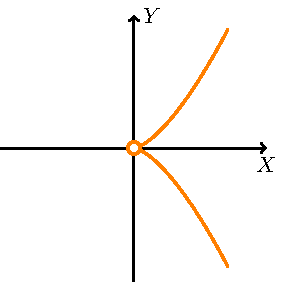
\includegraphics{Curve1.pdf}
		
		$Y^2=X^3$
	\end{minipage}
	\begin{minipage}{0.42\textwidth}
		\centering
		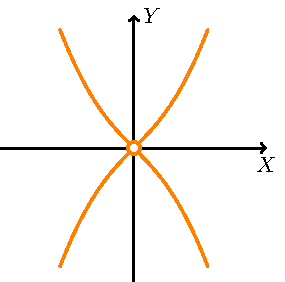
\includegraphics{Curve2.pdf}
		
		$Y^2=X^4+X^2$
	\end{minipage}
\end{center}

		
\begin{rem*}
    By Proposition~\reff{prop:dimLeqGeneratorsMaximal} and the proof of Proposition~\reff{prop:Jacobian}, 
    \begin{align*}
        \dim\left\{\nabla f(x)\st f\in I\right\} \leq \codim(X,k^n)\;.
    \end{align*}
\end{rem*}
\begin{rem}
    The $k$-vector space $\Nn = \left\{\nabla f(x) \st f\in I\right\}$ may be viewed as the \emph{conormal space} to $X$ at $x$ (at least if $X$ is regular at $x$) and its complement 
    \begin{align*}
        \Nn^\perp = \left\{ \xi = (\xi_i)_{i=1}^n \in k^n \st \sum_{i=1}^{n}\frac{\partial f}{\partial X_i}(x)\cdot\xi_i=0 \text{ for all } f\in I\right\}
    \end{align*}
    as the \emph{tangent space} at $x$ of $X$.
\end{rem}
\begin{thm}\lbl{thm:codimIneqRegular}
    Let $X\subseteq k^n$ be quasi-affine and $Y,Z \subseteq X$ be irreducible closed subsets and $C$ be any irreducible component of $Y\cap Z$. If there is at least one point $x\in C$ such that $X$ is regular at $x$, then 
    \begin{align*}
    	\codim(C,X) \leq \codim (Z,X)+\codim(Y,X)\;.
    \end{align*}
\end{thm}
\begin{rem}
    Let $n=4$, identify $k^4$ with the space of $2\times 2$-matrices and let $X= \left\{ A\st \det A = 0\right\}$. This has dimension 3 (where $X$ turns out to be irreducible), and 
    \begin{align*}
        Y = \left\{\begin{pmatrix} a&b\\ 0&0\end{pmatrix} \st a,b\in k \right\}\;,\quad
        Z = \left\{\begin{pmatrix} 0&0\\ c&d\end{pmatrix} \st c,d\in k \right\}
    \end{align*}  
    are irreducible closed subsets of codimension 1 and (thus) dimension 2. But $Y\cap Z = \{0\}$ has codimension 3 in $X$.
\end{rem}
\begin{proof}[Proof of Theorem \reff{thm:codimIneqRegular}]
	First of all, passing to the respective closures (which doesn't change codimension, e.g. by the \emph{locality of codimension}, cf. Remark~\reff{rem:proofPreparations}\itememph{a}), we may assume that $X,Y,Z$ are affine.
	
    \emph{Step 1.} As in the proof of Theorem~\reff{thm:codimIneq}, let $\Delta$ be the diagonal in $k^{2n}$. We will show the following: If $f_1,\ldots, f_d\in\Oo_{X,x}$ generate the maximal ideal $\mm_{X,x}$ of $\Oo_{X,x}$, then there exists an affine open neighbourhood $U$ of $x$ in $X$ and preimages of the $f_i$ in $\Oo(U)$ (which we will also call $f_i$) such that 
    \begin{align}\lbl{eq:conditionOnUxU}
        \Delta \cap (U\times U) = \left\{(y,z)\in U\times U \st f_i(y) = f_i(z) \text{ for } 1\leq i \leq d\right\}= V(g_1,\ldots,g_d)\tag{$*$}
    \end{align}
    (where $g_i(y,z)=f_i(y)-f_i(z)$), possibly after shrinking $U$. As $U$ is required to be \emph{affine open}, i.e. $U=X\setminus V(h)$ for some $h\in\Oo(X)$, we obtain that $Y\cap U=Y\setminus V(h|_Y)\eqqcolon Y'$ and $Z\cap U=Z\setminus V(h|_Z)\eqqcolon Z'$ are affine open as well, hence isomorphic to affine varieties (\cite[Proposition~2.2.4]{alg1}) and it makes sense to talk about vanishing sets of regular functions on $Y'$ and $Z'$ -- which we will do now. 
    
    Consider $\gamma_1,\ldots, \gamma_d\in\Oo(Y'\times Z')$, $\gamma_i(y,z)=f_i|_{Y'}(y)-f_i|_{Z'}(z)$ (this essentially restricts $g_1,\ldots, g_d$ to $Y'\times Z'$). We identify $Y\cap Z$ with $\Delta\cap (Y\times Z)$ and thus $C$ with its respective image, as we did in the proof of Theorem~\reff{thm:codimIneq}. Hence $C$ is an irreducible component of $\Delta\cap (Y\times Z)$. Then $C'=C\cap (U\times U)$ is an irreducible component of $\Delta\cap (Y'\times Z')=V(\gamma_1,\ldots,\gamma_d)$ (here we used \eqreff{eq:conditionOnUxU}) and Theorem~\reff{thm:krullIdeal} together with \emph{locality of codimension} yields
    \begin{align*}
    	\codim(C,Y\times Z)=\codim(C',Y'\times Z')\leq d\;.
    \end{align*}
    We silently went over an important detail: $U\times U\subseteq X\times X$ is open again. This is easily seen as $(X\setminus U)\times X$ and $X\times (X\setminus U)$ are closed (using e.g. the argument from the proof of Proposition~\reff{prop:codimensionProduct}), but don't be fooled: this \emph{does not} follow from \emph{product topology stuff}; the Zariski topology on $k^{2n}$ and $X\times X$ is \emph{not} the product of the Zariski topologies on $k^n$ or $X$. 
    
    Enough of that. From Proposition~\reff{prop:codimensionProduct} we get
    \begin{align*}
    	\codim(Y\times Z,X\times X)&=\dim(X\times X)-\dim(Y\times Z)\\
    	&=(\dim (X)-\dim (Y))+(\dim (X)-\dim (Z))\\
    	&=\codim(Y,X)+\codim(Z,X)
    \end{align*}
    and hence, 
    \begin{align*}
        \codim(C,X)& = \dim(X) -\dim(C)\\
        &= \dim (X) - (\dim(X)+\dim(X) -\codim(C,X\times X))\\
        &= \codim(C,X\times X) -\dim (X)\\
        &=\codim(C,Y\times Z)+\codim(Y\times Z,X\times X)-\dim (X)\\
        &\leq \codim(Y,X) +\codim(Z,X) +d-\dim(X) \\
        &=\codim(Y,X) +\codim(Z,X),
    \end{align*}
    provided that $d=\dim(X)$, which is possible for an appropriate choice of the $f_i$ when $X$ is regular at $x$ (by \NAK, $\mm_{X,x}$ can be generated by $\dim (X)$ elements, cf. the proof of Proposition~\reff{prop:dimLeqGeneratorsMaximal} or \cite[Concluding remarks, Lemma~1\itememph{c}]{alg1}).
    
    \emph{Step 2.} Let $R= k[X_1,\ldots, X_m]$ and $\pp,\mm\subseteq R$ be the prime ideal defining $k^\ell \times \{0\}^{m-\ell}$ respectively the maximal ideal defining $\{0\}^m$. Then $\mm^2 \cap \pp \subseteq \mm\cdot\pp$. This can be shown as follows. Since $\mm$ is generated by $X_1,\ldots,X_m$, $\mm^2$ is generated by the $X_iX_j$ (with $i,j$ not necessarily distinct). Similarly, $\pp$ is the ideal generated by $X_{\ell+1},\ldots, X_m$. If $f\in R$ lies in both $\mm^2$ and $\pp$, each monomial of $f$ must be divisible by some $X_iX_j$ as well as by some $X_{\ell+r}$. Then this monomial is divisible by $X_iX_{\ell+r}$ or $X_jX_{\ell+r}$, hence contained in $\mm\cdot\pp$. Now $f\in\mm\cdot\pp$ because each monomial lies in that ideal.
       
   \emph{Step 3.} Let $\xi\in k^m$, $L\subseteq k^m$ an affine subspace containing $\xi$. Let $\pp$ be the prime ideal defining $L$ and $\mm$ the maximal ideal defining $\{\xi\}$. Then $\pp\cap \mm^2 \subseteq I\cdot \mm$. This can be reduced to the previous step by an affine automorphism of $k^m$.
    
    \emph{Step 4.} Let $x\in k^n$, $\mm_x \subseteq S= k[X_1,\ldots, X_n]$ the maximal ideal defined by $x$, $f_1,\ldots, f_n\in S$ such that their images generate $\mm_x/\mm_x^2$. Then there is $h\in R = k[X_1,\ldots, X_n,Y_1,\ldots Y_n]$ such that $h(x,x) \neq 0$ and $h\cdot \pp_\Delta \subseteq (g_1,\ldots, g_n)_R$ where $g_i(y,z) = f_i(y)-f_i(z)$ and $\pp_\Delta\subseteq R$ is the prime ideal of functions vanishing on $\Delta = \left\{(y,y)\st y\in k^n\right\}$. To see this, let $\xi = (x,x)$ and $\qq = \pp_\Delta \cdot R_{\mm_\xi}$, where $\mm_\xi\subseteq R$ denotes the maximal ideal of functions vanishing on $\xi$. Let $\nn = \mm_\xi\cdot R_{\mm_\xi}$ denote the maximal ideal of the local ring $R_{\mm_\xi}$. From the previous step it follows that 
    \begin{align}\lbl{eq:thm15}
        \nn^2\cap \qq\subseteq \qq\cdot \nn .
    \end{align}
    Let $\gg\subseteq \qq$ be the ideal generated by the images of the $g_i$. Our long-term goal is to show $\gg=\pp$. Let $f\in \pp_\Delta$. We claim that there are $c_1,\ldots,c_n$ such that $g=f-\sum_{i=1}^n c_i g_i$ is in $\mm_\xi^2$. Indeed, by the isomorphism \eqreff{eq:modToNabla} this is equivalent to $\nabla g(\xi)=0$. Since $f|_\Delta = 0$, we have $\frac{\partial f}{\partial X_i}(\xi) + \frac{\partial f}{\partial Y_i}(\xi) = 0$ at $\xi\in \Delta$ and the same for the $g_i$. Thus, it is sufficient to have 
    \begin{align*}
        \frac{\partial f}{\partial X_i}(\xi) = \sum_{j=1}^n c_j \frac{\partial g_j}{\partial X_i}(\xi) = \sum_{j=1}^n c_j \frac{\partial f_j}{\partial X_i}(x)\quad\text{for all }i=1,\ldots,n
    \end{align*}
    (the second equality is tautological), which is possible since the $f_i$ generate $\mm_x/\mm_x^2$, hence the $\nabla f_i(x)$ generate $k^n$ by the isomorphism \eqreff{eq:modToNabla}. It follows that $\pp_\Delta\subseteq (g_1,\ldots,g_n)_R + (\pp_\Delta\cap \mm_\xi^2) = (g_1,\ldots,g_n) + \pp_\Delta\cdot \mm_\xi$ (the second equality follows from Step 3). This is still true in the localization at $\mm_\xi$, i.e. $\qq\subseteq \gg +\qq\cdot\nn$. By Corollary \reff{cor:NAK}, we have $\qq= \gg$. 
    
    Now let $\phi_1,\ldots,\phi_N$ generate $\pp_\Delta$. Since $\qq =\pp_\Delta\cdot R_{\mm_\xi}$ is generated by the images of the $g_i$, there are $h_i\not\in \mm_\xi$ and such that $h_i\cdot \phi_i \in(g_1,\ldots,g_n)_R$. Then $h=h_1\cdots h_N$ fulfills $h(\xi)=h(x,x)\not=0$ and $h\cdot\pp_\Delta\subseteq(g_1,\ldots,g_n)_R$.
    
    \emph{Step 5.} Let $f_1,\ldots, f_d$ be elements of $S= k[X_1,\ldots, X_n]$ such that their images in $\Oo_{X,x}$ form a base of $\mm_{X,x}/\mm_{X,x}^2$ (again, $\mm_{X,x}$ is the maximal ideal of the local ring $\Oo_{X,x}$, which Professor Franke would like to express as $\mm_{X,x}=\rad \Oo_{X,x}$). Let $f_{d+1},\ldots, f_n$ be chosen in such a way that the images of $f_1,\ldots, f_n$ form a base of $\mm_x/\mm_x^2$. Why is this possible? We have $\mm_{X,x}/\mm_{X,x}^2=\nn/\nn^2$, $\nn\subseteq\Oo(X)$ denoting the maximal ideal of $\Oo(X)$ of functions vanishing at $x$. Then $\nn/\nn^2$ is a quotient of $\mm_x/\mm_x^2$ (as we saw in the proof of Proposition~\reff{prop:Jacobian}). If $h$ is as in the previous step, $U= X\setminus V(h)$ has the required property.
\end{proof}
\begin{rem}[on \eqreff{eq:thm15}]
    Let $R$ be an arbitrary ring, $S\subseteq R$ a multiplicative subset, $I$ and $J$ ideals in $R$. Then 
    \begin{align*}
        (I+J) \cdot R_S &= I\cdot R_S + J \cdot R_S\\
        (I\cap J)\cdot R_S &= I\cdot R_S \cap J\cdot R_S\\
        (I\cdot J)\cdot R_S &= (I\cdot R_S)\cdot(J\cdot R_S)\\
        \sqrt{I\cdot R_S}&= \sqrt{I}\cdot R_S
    \end{align*}
\end{rem}
\begin{proof}
    We will only prove the second equality, they are all quite similar. The image of $I\cap J$ is contained in both $I\cdot R_S$ and $J\cdot R_S$, hence so is $(I\cap J)\cdot R_S$, proving $(I\cap J) \cdot R_S \subseteq I\cdot R_S \cap J\cdot R_S$. Conversely, let $\rho \in (I \cdot R_S)\cap (J\cdot R_S)$. Since $\rho\in I\cdot R_S$, $\rho = \frac{i}{s}$ where $i\in I$ and $s\in S$. Since $\rho\in J\cdot R_S$, $\rho = \frac{j}{t}$ where $j\in J$ and $t\in S$. Since $\frac{i}{s}=\frac{j}{t}$ in $R_S$, there is $\sigma \in S$ such that $\sigma i t = \sigma  j  s$. Then $\rho = \frac{\sigma  i t}{\sigma  s t} = \frac{\sigma  j s}{\sigma  s t}\in (I\cap J)\cdot R_S$.
\end{proof}



\section{Derivations and the module of Kähler differentials}
\begin{defi}[Derivations]\lbl{def:derivation}
    Let $A$ be a ring, $M$ an $A$-module, $d\colon A\to M$  a homomorphism of the additive group. We say that $d$ is a \defemph{derivation} of $A$ with values in $M$ if it satisfies the \emph{Leibniz rule} 
    \begin{align*}
    	 d(a\cdot b) = b\cdot d(a) + a\cdot d(b)\;.
    \end{align*}
     If $A$ is an $R$-algebra and $A\morphism[d] M$ a derivation of $A$, we call $d$ \emph{$R$-linear} if the following equivalence conditions hold:
    \begin{alphanumerate}
        \item 
            $d(r) = 0$ for all $r\in R$.
        \item
            $d(r\cdot a) = r\cdot d(a)$ for all $r\in R, a\in A$.
    \end{alphanumerate}
    Let $\Der(A,M)$ denote the set of derivations with values in $M$. This can be given a canonical $A$-module structure via $(a\cdot d)(b) = a\cdot d(b)$.
\end{defi}
\begin{proof}
    Let $d\in \Der(A,M)$. Note that we always have $d(1)=0$ as $d(1)=d(1\cdot1)=d(1)+d(1)$ by the Leibniz rule. Now, assuming $d(r\cdot a)=r\cdot d(a)$ for all $r\in R, a\in A$, we obtain $d(r)=d(r\cdot1)=0$. Conversely, if $d(r)=0$ for all $r\in R$, then $d(a\cdot r) = a\cdot d(r) + r\cdot d(a) = r\cdot d(a)$ by the Leibniz rule. Hence, \itememph{a} and \itememph{b} are indeed equivalent.
\end{proof}
\begin{rem}
    The set $\Der_R(A,M)$ of $R$-linear derivations forms an $A$-submodule of $\Der(A,M)$.
\end{rem}
\begin{example}\lbl{ex:universalDerivationPolynomialRing}
    A derivation $d\in\Der_R(R[X_1,\ldots,X_n], M)$ is uniquely determined by the tuple $(m_1,\ldots,m_n)\in M^n$ via
    \begin{align*}
        d&\longmapsto (dX_1,\ldots,dX_m)\\
        \bigg(P\mapsto \sum_{i=1}^n\frac{\partial P}{\partial X_i}\cdot m_i \bigg) &\longmapsfrom (m_1,\ldots,m_n)\;.
    \end{align*}
    Note that the left hand side is indeed a derivation:
    \begin{align*}
        d(PQ) = \sum_{i=1}^n \frac{\partial(PQ)}{\partial X_i} \cdot m_i = \sum_{i=1}^n \left( P \cdot\frac{\partial Q}{\partial X_i} + Q\cdot\frac{\partial P}{\partial X_i} \right) m_i = P\cdot d(Q) + d(P)\cdot Q\;.
    \end{align*}
    It is easy to see that the two maps are inverse to each other.
\end{example}
\begin{rem*}
    $\Der(A,-)$ and $\Der_R(A,-)$ are functors: If $M\morphism[\mu] N$ is a homomorphism of $A$-modules then 
    \begin{align*}
        \Der(A,M) &\longto \Der(A,N)\\
        d &\longmapsto \mu \circ d
    \end{align*}
    is a morphism of $A$-modules and similar for $\Der_R(A,M)$ and $\Der_R(A,N)$.
    
    The previous Example~\reff{ex:universalDerivationPolynomialRing} can be re-formulated as saying that
    \begin{align*}
        d\colon A = R[X_1,\ldots, X_n] &\longto A^n\\
        P &\longmapsto \nabla P=\bigg(\frac{\partial P}{\partial X_1},\ldots,\frac{\partial P}{\partial X_n}\bigg)
    \end{align*}
    is the \emph{universal} $R$-linear derivation of $A$: Any $\delta \in \Der_R(A,M)$ can be uniquely expressed as $\delta = \mu \circ d$ where $A^n \morphism[\mu] M$ is a uniquely determined $A$-linear homomorphism.
\end{rem*}
\begin{defi}[Kähler differentials] \lbl{def:KahlerDiff}
    Let $A$ be an $R$-algebra. A \defemph{module of Kähler differentials} for $A/R$ is an $A$-module $\Omega_{A/R}$ together with $d_{A/R} \in \Der_R(A,\Omega_{A/R})$ satisfying the following universal property: 
    \begin{quote}
    	For any $A$-module $M$ and any $\delta \in \Der_R(A,M)$ there is a unique $A$-homomorphism $\Omega_{A/R}\morphism[\epsilon] M$ such that
    	\begin{diagram*}
    		\node[ob](A) at (0,1.25) {$A$};
    		\node[ob](M) at (2.5,1.25) {$M$};
    		\node[ob](O) at (1.25,0) {$\Omega_{A/R}$};
    		\scriptsize
    		\draw[->] (A) -- (M) node[pos=0.5, above] {$\delta$};
    		\draw[->] (A) -- (O) node[pos=0.5, below left] {$d_{A/R}$};
    		\draw[->, dashed] (O) -- (M) node[pos=0.5, below right] {$\exists!\ \epsilon$};
    	\end{diagram*}
    \end{quote}
     It is worth pointing out that we thus defined $\Omega_{A/R}$ by an \emph{$(\epsilon,\delta)$-definition}!
\end{defi}
\begin{rem*}
    \begin{alphanumerate}
        \item 
            The universal property characterizes $\Omega_{A/R}$ up to unique isomorphism (if it exists): If $\snake d_{A/R} \in\Der_R(A,\snake \Omega_{A/R})$ has the same universal property, there is a unique isomorphism $\Omega_{A/R}\isomorphism[i] \snake \Omega_{A/R}$ such that $\snake d _{A/R} = i \circ d_{A/R}$. In fact, the universal property of $d_{A/R}$ shows the existence and uniqueness of a homomorphism $i$ with this property. Reversing the roles of $d_{A/R}$ and $\snake d_{A/R}$ we also obtain $\snake\Omega_{A/R} \morphism[j]\Omega_{A/R}$ such that $d_{A/R} = j\circ \snake d_{A/R}$. Then $\alpha = j\circ i$ satisfies $d_{A/R} = \alpha\circ d_{A/R}$ which implies $\alpha= \id_{\Omega_{A/R}}$ by the universal property of $\Omega_{A/R}$. Exchanging $d_{A/R}$ and $\snake d_{A/R}$ gives $i \circ j = \id_{\snake\Omega_{A/R}}$. Thus, $i$ is an isomorphism.
        \item
            For $A= R[X_1,\ldots,X_n]$, $\Omega_{A/R} = \bigoplus_{i=1}^n A\cdot dX_i \simeq A^n$ with $d_{A/R} (P) = \sum_{i=1}^n \frac{\partial P }{\partial X_i} \cdot dX_i$ is a module of Kähler differentials.
        \item 
            If $A$ is a quotient of $R$ (i.e. $R\morphism A$ is surjective) then $\Der_R(A,M) = 0$ for all $M$, hence $\Omega_{A/R} = 0$.
    \end{alphanumerate}
\end{rem*}
\begin{defi}[Free module] \lbl{def:freeModule}
    The free $A$-module $F$ with generating set $M$, $F=\bigoplus_{m\in M}A$, is the $A$-module of functions $f\colon M \morphism A$ with finite support. We define $\delta_x \in F$ by $\delta_x(y) = \delta_{x,y}$ (i.e. $\delta_x(x)=1$ and $\delta_x(y)=0$ for $y\not=x$).
\end{defi}

\begin{rem*}
    \begin{alphanumerate}
        \item  
            One often thinks of $F$ as the module of formal (finite) $A$-linear combinations of $M$ with $f=\sum_{x\in M} f(x) x$ instead of $f= \sum_{x\in M} = f(x)\delta_x$.
        \item 
            We have a bijection, for any $A$-module $N$,
            \begin{align*}
                \Hom_{\cat{Set}}(M,N) &\isomorphism \Hom_A(F,N)\\
                \upsilon &\longmapsto \bigg(f\mapsto \sum_{m\in M} f(m) \upsilon(m)\bigg)\\
                \big(m\mapsto \phi(\delta_m) \big) &\longmapsfrom \phi\;.
            \end{align*}
            In other words, mapping $X$ to the free $A$-module generated by $X$ as a functor from $\cat{Set}$ to the category of $A$-modules is \emph{left-adjoint} to the forgetful functor from the category of $A$-modules to $\cat{Set}$.
    \end{alphanumerate}
\end{rem*}

\begin{prop}\lbl{prop:kahlerExists}
    A module $\Omega_{A/R}$ of Kähler differentials  exists for any $R$-algebra $A$.
\end{prop}
\begin{proof}
    %If $(A\morphism[d] M) \in \Der_R(A,M)$ it defines a unique $F_A\morphism[c] M$ where $F_A$ is the free $A$-module generated by $A$, such that $d(a) = c(\delta_a)$.
    We follow the \emph{brute-force} approach to constructing $\Omega_{A/R}$. Let $F_A$ be the free $A$-module generated by the set $A$ itself and let $K\subseteq F_A$ the submodule generated by the following three types of elements:
    \begin{alphanumerate}
        \item 
            $\left\{\delta_x+\delta_y-\delta_{x+y}\st x,y\in A\right\}$
        \item 
            $\left\{\delta_r\st r\in R\right\}$
        \item 
            $\left\{x\delta_y+y\delta_x -\delta_{xy} \st x,y\in A\right\}$
    \end{alphanumerate}
    Let $\Omega_{A/R} = F_A/K$, $F\morphism[\pi] \Omega_{A/R}$ be the projection to the quotient and put $d_{A/R}(a) = \pi(\delta_a)$. It is easy to see that $d_{A/R}\in \Der_R(A,M)$ e.g.
    \begin{align*}
        d_{A/R}(ab) = \pi(\delta_{ab}) = \pi(\delta_{ab}-a\delta_b -\delta_a) + a\pi(\delta_b) +b\pi(\delta_a) = a\cdot d_{A/R}(b) + b\cdot d_{A/R}(a)
    \end{align*}
    as $\delta_{ab}-a\delta_b -\delta_a\in K$ and by the definition of $d_{A/R}$.
    
    Let $(A\morphism[d] M)\in \Der_R(A,M)$. By the universal property of $F_A$ there is a unique morphism $c\in \Hom_A(F_A,M)$ such that $d(a) = c(\delta_a)$. We claim that $c$ vanishes on $K$.
    \begin{itemize}
      \item 
        $c(\delta_a +\delta_b -\delta_{a+b}) = c(\delta_a) +c(\delta_b) -c(\delta_{a+b}) = d(a)+d(b)-d(a+b) = 0$ as $d$ is additive.
      \item 
        $c(\delta_r) = d(r) = 0$ when $r\in R$ as $d$ is $R$-linear.
      \item 
        $c(a\delta_b+b\delta_a -\delta_{ab}) = a\cdot d(b) + b\cdot d(a) - d(ab) = 0$ by the Leibniz rule.
    \end{itemize}
    Consequently, due to the universal property of quotient modules, there is a unique $\delta\in \Hom_A(F_A/K , M)$ such that 
    \begin{diagram*}
    	\node[ob](FA) at (0,1.25) {$F_A$};
    	\node[ob](M) at (2.5,1.25) {$M$};
    	\node[ob](O) at (1.25,0) {$F_A/K$};
    	\scriptsize
    	\draw[->] (FA) -- (M) node[pos=0.5, above] {$d$};
    	\draw[->] (FA) -- (O) node[pos=0.5, below left] {$\pi$};
    	\draw[->, dashed] (O) -- (M) node[pos=0.5, below right] {$\exists!\ \delta$};
    \end{diagram*}
    commutes. Therefore, $F_A/K=\Omega_{A/R}$ satisfies the universal property.
\end{proof}
In many cases, the module of Kähler differentials can be calculated using $\Omega_{R[X_1,\ldots,X_n]}\simeq \bigoplus_{i=1}^n R[X_1,\ldots, X_n] dX_i$ and two exact sequences which follow in a straight forward way from
\begin{fact}\lbl{fact:DerExactSequences}
    Let $R$ be a ring, $A$ an $R$-algebra.
    \begin{alphanumerate}
        \item 
            Let $I\subseteq A$ be any ideal, $M$ any $A/I$-module, $A\morphism[\pi]A/I$ the projection, then 
            \begin{align}\lbl{eq:derExactSequence1}
                0\morphism \Der_R(A/I,M) \morphism \Der_R(A,M) \morphism \Hom_{A/I}(I/I^2, M) 
            \end{align}
            is exact. Herein, the morphism $\Der_R(A/I,M) \morphism \Der_R(A,M)$ is defined by $d\mapsto \delta=d\circ\pi$ and $\Der_R(A,M) \morphism \Hom_{A/I}(I/I^2, M)$ by $\delta\mapsto\phi = \left(i\mod I^2\mapsto\delta(i)\right)$.
        \item 
            Let $B$ be an $A$-algebra, $M$ an $B$-module, then we have the exact sequence
            \begin{align}\lbl{eq:derExactSequence2}
	            \begin{split}
		            0 \morphism \Der_A(B,M) \monomorphism\Der_R(B,M) &\morphism \Der_R(A,M)\\
		            d&\longmapsto d|_A\;.
	            \end{split}
            \end{align}
    \end{alphanumerate}
\end{fact}
\begin{proof}
    We will first proof \itememph{b}. The exactness on the left end is obvious, as is the vanishing of the composition $\Der_A(B,M) \monomorphism \Der_R(B,M) \morphism \Der_R(A,M)$. Let $d\in \Der_R(B,M)$ such that $0 = d|_A$, then $d$ is $A$-linear, i.e. $d\in \Der_A(B,M)$.
    
    Now about \itememph{a}. That $\Der_R(A/I,M) \morphism \Der_R(A,M)$ is well-defined is obvious, as derivations are compatible with applying ring homomorphisms on the right. To show that the rightmost arrow is well-defined, we first need to show that $\delta\in\Der_R(A,M)$ vanishes on $I^2$. If $i,j\in I$, then $\delta(i\cdot j)=i\cdot\delta(j)+j\cdot\delta(i)=0$ as $I\cdot M=0$, hence $\delta$ indeed vanishes on $I^2$ as $I^2$ is generated by the $ij$ where $i,j\in I$. It follows that $\phi$ is indeed a homomorphism of abelian groups. Let $\alpha = a\mod I\in A/I$ and $i\in I$, then $\phi(\alpha \cdot (i\mod I^2)) = \delta(a\cdot i) = i\cdot \delta(a) + a\cdot \delta(i) = \alpha\cdot\delta(i)$ showing that $\phi$ is $(A/I)$-linear as stated. 
    
    Exactness on the left end follows from the surjectivity of $A\morphism[\pi] A/I$. The fact that the composition $d\in\Der_R(A/I,M)\mapsto\delta\in\Der_R(A,M)\mapsto\phi\in\Hom_{A/I}(I/I^2,M)$ is zero is also obvious: $\phi(i\mod I^2) = \delta(i) = d(\pi(i)) = d(0) = 0$. Finally, let $\delta$ be such that $\phi = 0$. For $i\in I$, $\delta(i) = \phi(i\mod I^2) = 0$. Hence there exists a unique group homomorphism $A/I \morphism[d] M$ such that $\delta = d\circ \pi$. The Leibniz rule for $d$ follows from the analogous rule for $\delta$ and the surjectivity of $\pi$.
\end{proof}
\begin{fact*}\lbl{fact:HomRightExact}
    Let $A$ be any ring, $M'\morphism M\morphism M''\morphism 0$ a sequence of $A$-homomorphisms, then this sequence is exact iff $0\morphism\Hom_A(M'',T) \morphism \Hom_A(M,T) \morphism\Hom_A(M',T)$ is exact for any $A$-module $T$.
\end{fact*}
\begin{cor}\lbl{cor:kahlerExactSequences}
    Let $R$ be a ring, $A$ an $R$-algebra. 
    \begin{alphanumerate}
        \item 
            If $I\subseteq A$ is any ideal, we have a canonical short exact sequence of $(A/I)$-modules
            \begin{align}\lbl{eq:tensorDerSpam1}
                I/I^2\morphism[\alpha] \Omega_{A/R} \otimes_A A/I \morphism[\beta] \Omega_{(A/I)/R} \morphism 0\;.
            \end{align}
        \item 
            If $B$ is any $A$-algebra, we have a canonical short exact sequence of $B$-modules
            \begin{align}\lbl{eq:tensorDerSpam2}
                \Omega_{A/R}\otimes_A B \morphism[\kappa] \Omega_{B/R} \morphism[\lambda] \Omega_{B/A} \morphism 0\;.
            \end{align}
    \end{alphanumerate}
\end{cor}
\begin{rem*}
    \begin{alphanumerate}
        \item 
            Tensor products as occuring above are used for change of base: $M\otimes_A B$ is a $B$-module together with a morphism $M\morphism M\otimes_A B$, $m \mapsto m \otimes_A 1$ with the following universal property: 
            \begin{quote}
            	If $T$ is any $B$-module and $M\morphism[\tau] T$ any $A$-linear homomorphism, then there is a unique homomorphism $M\otimes_A B \morphism[t] T$ such that
            	\begin{diagram*}
            		\node[ob](M) at (0,1.25) {$M$};
            		\node[ob](T) at (2.5,1.25) {$T$};
            		\node[ob](MB) at (1.25,0) {$M\otimes_AB$};
            		\scriptsize
            		\draw[->] (M) -- (T) node[pos=0.5, above] {$\tau$};
            		\draw[->] (M) -- (MB) node[pos=0.5, below left] {$-\otimes_A1$};
            		\draw[->, dashed] (MB) -- (T) node[pos=0.5, below right] {$\exists!\ t$};
            	\end{diagram*}
            	 commutes, i.e. $\tau(m) = t(m\otimes_A 1)$. In particular, there is an isomorphism $\Hom_A(M,T)\simeq\Hom_B(M\otimes_AB,T)$ of $B$-modules.
            \end{quote}
            For instance, $V\otimes_\IR \IC$ is the complexification of the $\IR$-vector space $V$. We put $m\otimes_A b= b\cdot (m\otimes_A 1)$. One easy special case is $B=A/I$ in which case 
            \begin{align*}
            	M\otimes_A(A/I)=M/(I\cdot M)\;, \quad m\otimes_A (a\mod I) \coloneqq (a\cdot m) \mod (I \cdot M)
            \end{align*}
            has the desired universal property. More about tensor products may be found in the appendix, section~\reff{sec:tensorProducts}.
        \item
            Using and \reff{eq:tensorDerSpam1} the calculation of $\Omega_{R[T_1,\ldots,T_n]/R}$ it is possible to calculate $\Omega_{(A/I)/R}$ (where $A=R[T_1,\ldots, T_n]$) as the cokernel of 
            \begin{diagram*}
            	\node[ob](I) at (0,1.25) {$I/I^2$};
            	\node[ob](O) at (2,1.25)  {$\Omega_{A/R}\rlap{$/(I\cdot\Omega_{A/R})$}$};
            	\node[ob](A) at (2, 0) {$(A/I)^n$};
            	\path (A) -- (O) node[pos=0.5, sloped] {$\simeq$};
            	\scriptsize
            	\path (I) ++ (-1.75,-0.25) node (i) {$f\mod I^2$};
            	\path (A) ++ (-1.75,-0.25) node (a) {$\nabla f\mod I$};
            	\draw[->] (I) -- (O);
            	\draw[->] (I) -- (A);
            	\draw[|->] (i) -- (a);
            \end{diagram*}
            Since any $R$-algebra of finite type has the form $A/I$, this provides a way to calculate $\Omega_{B/R}$ for such $R$-algebras $B$. Since Example \reff{ex:universalDerivationPolynomialRing} is not (really) limited to case of finitely many variables, other $R$-algebras could be treated as well.
    \end{alphanumerate}
\end{rem*}
\begin{proof}[Proof of Corollary~\reff{cor:kahlerExactSequences}]
	Let us first construct the involved canonical homomorphisms.
	\begin{itemize}
		\item 
		By the universal property of $d_{B/R}$, the derivation $d_{B/A}\colon B\morphism \Omega_{B/A}$ (which is $R$-linear) hence has a unique representation 
		\begin{align*}
			d_{B/A} = \lambda \circ d_{B/R}\;,
		\end{align*}
		in which $\lambda$ is an $B$-homomorphism $\Omega_{B/R}\morphism[\lambda]\Omega_{B/A}$.
		 \item 
		 Composing $d_{B/R}\colon B \morphism \Omega_{B/R}$ with $A\morphism B$ gives us an element of $\Der_R(A, \Omega_{B/R})$, which, by the universal property of $\Omega_{A/R}$, is given by a unique $A$-module-homomorphism 
		 \begin{align*}
		 	\Omega_{A/R} \morphism[\kappa'] \Omega_{B/R}\;.
		 \end{align*}
		 By the universal property of $-\otimes_A B$, $\kappa'$ is given by a unique $B$-module-homomorphism
		 \begin{align*}
		 	\Omega_{A/R} \otimes_A B \morphism[\kappa] \Omega_{B/R}\;.
		 \end{align*}
		 In other words, $\kappa$ is the unique $B$-module-homomorphism such that $\kappa(d_{A/R}(a)\otimes_A b) = b\cdot d_{B/R}(a)$.
		 \item 
		 The $A/I$-homomorphism $\beta$ is uniquely determined by 
		 \begin{align*}
		 	\beta\left(d_{A/R}(a) \mod (I\cdot \Omega_{A/R})\right) = d_{(A/I)/R}(a)\;.
		 \end{align*}
		 In other words, this is the special case $B=A/I$ of $\kappa$.
		 \item 
		 We put 
		 \begin{align*}
		 	\alpha(i\mod I^2) = d_{A/R}(i) \mod (I\cdot \Omega_{A/R})\;.
		 \end{align*}
		 In other words, $\alpha$ is obtained by applying $\Der_R(A,M) \morphism \Hom_{A/I} (I/I^2, M)$ from Fact~\reff{fact:DerExactSequences} to the derivation $A\xrightarrow{\smash{d}_{A/R}} \Omega_{A/R} \morphism \Omega_{A/R}/I \cdot \Omega_{A/R} \eqqcolon M$.
	\end{itemize}
	It remains to show exactness. By \hyperref[fact:HomRightExact]{this} unnamed fact, it is sufficient to show that exactness holds after applying the functor $\Hom_B(-,T)$ for any $B$-module $T$ (where in \itememph{a} we have the special case $B=A/I$). Note that 
	\begin{align*}
		\Hom_A\left(\Omega_{A/R},T\right)\simeq\Der_R(A,T)\quad\text{and}\quad \Hom_B\left(\Omega_{A/R}\otimes_AB,T\right)\simeq \Hom_A\left(\Omega_{A/R},T\right) 
	\end{align*}
	by the universal properties of $\Omega_{A/R}$ and $-\otimes_AB$. Hence, applying $\Hom_B(-,T)$ transforms \eqreff{eq:tensorDerSpam1} and \eqreff{eq:tensorDerSpam2} into \eqreff{eq:derExactSequence1} and \eqreff{eq:derExactSequence2} respectively, thus showing exactness by Fact~\reff{fact:DerExactSequences}. 
\end{proof}
\begin{varthm}{fact}\lbl{fact:DerLocalization}
	This should actually be in Fact~\reff{fact:DerExactSequences}, but we refuse to change a fact that was stated two lectures ago.
    \begin{itemize}
      \item[\itememph{c}]
        When $X\subseteq R$ is multiplicative and $M$ an $A_X$-module, then we have an isomorphism of $A_X$-modules
        \begin{align}\lbl{eq:DerLocalizationIso1}
            \Der_{R_X}(A_X,M) \isomorphism \Der_R(A,M).
        \end{align}
      \item[\itememph{d}]
        When $S\subseteq A$ is multiplicative and $M$ an $A_S$-module, then we have an isomorphism of $A_S$-modules
        \begin{align}\lbl{eq:DerLocalizationIso2}
            \Der_R(A_S,M)\isomorphism \Der_R(A,M).
        \end{align}
    \end{itemize}
\end{varthm} 
\begin{proof}
    Both maps are defined by composition of derivations with the ring homomorphisms $A\morphism A_X$ respectively $A\morphism A_S$, so they are well-defined.
    
    To prove \itememph{c}, take any element $d\in \Der_R(A,M)$. This is $R$-linear and hence defines a unique homomorphism $A_X\morphism[d] M$ of $R_X$ modules, by our assumption on $M$ and the universal property of the localization. To confirm the Leibniz rule, look at
    \begin{align*}
        d\left(\frac{a}{x}\cdot \frac{\alpha}{\xi}\right) = \frac{d(a\cdot\alpha)}{x\cdot \xi} = \frac{\alpha\cdot d(a) +a\cdot d(\alpha)}{x\cdot \xi} = \frac{\alpha}{\xi}\frac{d(a)}{x} +\frac{a}{x}\frac{d(\alpha)}{\xi} = \frac{\alpha}{\xi}d\left(\frac{a}{x}\right) +\frac{a}{x}d\left(\frac{\alpha}{\xi}\right).
    \end{align*}
    This proves surjectivity and injectivity follows from the uniqueness of $d$.
    
    To show \itememph{d}, let $d\in\Der_R(A_S,M)$ be an element of the kernel, then $d(a)$ when $a$ is in the image of $A$ in $A_S$. Let $\alpha\in A_S$, then there is $\sigma$ in the image of $S$ in $A_S$ such that $\sigma\cdot \alpha$ is in the image of $A$ in $A_S$. Then 
    \begin{align*}
        0 = d(\sigma\cdot \alpha) = \sigma \cdot d(\alpha) + \alpha\cdot d(\sigma) = \sigma\cdot d(\alpha)
    \end{align*}
    implies $d(\alpha) = 0$ since $\sigma\in (A_S)^\times$. This shows injectivity of the map. For surjectivity, let $\delta\in \Der_R(A,M)$ and put $d\left(\frac{a}{s}\right) = \frac{s\cdot\delta(a) - a\cdot\delta(s)}{s^2}$ (the \emph{quotient rule}). We have
    \begin{align*}
        d\left(\frac{\sigma\cdot a}{\sigma \cdot s}\right) = \frac{\sigma\cdot s\cdot \delta(\sigma\cdot a) - \sigma \cdot a \cdot \delta(\sigma\cdot s)}{\sigma^2\cdot s^2} = \frac{s\cdot \delta(a)-a\cdot\delta(s)}{s^2}
    \end{align*}
    showing that $d\colon A_S\morphism M$ is well-defined. That $d(R)=0$ is trivial, as is the additivity and the Leibniz rule is easily verified.
\end{proof}
\begin{varthm}{cor}
	Same as Fact~\reff{fact:DerLocalization}, this should have been stated a long time ago.
    \begin{alphanumerate}
        \item[\itememph{c}]
	        When $X\subseteq R$ is multiplicative, there is a canonical isomorphism of $A_X$-modules
	        \begin{align}\lbl{eq:KahlerLocalizationIso1}
		        \Omega_{A_X/R_X} \lisomorphism[\iota] (\Omega_{A/R})_X=\Omega_{A/R}\otimes _AA_X
	        \end{align}
	        (as $A_X=A\otimes R_X$, we could have taken the tensor product $-\otimes_RR_X$ as well).           
        \item[\itememph{d}]
	        When $S\subseteq A$ is multiplicative, there is a canonical isomorphism of $A_S$-modules
	        \begin{align}\lbl{eq:KahlerLocalizationIso2}
		        \Omega_{A_S/R} \lisomorphism(\Omega_{A/R})_S=\Omega_{A/R}\otimes_A A_S\;.
	        \end{align}
    \end{alphanumerate}
\end{varthm}
\begin{proof}
	As in the proof of Corollary~\reff{cor:kahlerExactSequences}, we should first agree on how the morphisms are supposed to look like.
	\begin{itemize}
		\item As $A\morphism A_X \xrightarrow{d_{A_X/R_X}} \Omega_{A_X/R_X}$ is an $R$-linear derivative of $A$, there is a unique morphism $\Omega_{A/R}\morphism[\alpha] \Omega_{A_X/R_X}$ of $A$-modules such that the left of the below diagrams commutes. By the universal property of the localization $\Omega_{A/R}\morphism(\Omega_{A/R})_X=\Omega_{A/R}\otimes_AA_X$ there is a unique $A_X$-module homomorphism $\iota$ such that the right diagram commutes.
		\begin{center}
			\begin{minipage}{0.4\textwidth}
				\centering				
				\begin{diagram*}
					\node[ob](A) at (0,1.5) {$A$};
					\node[ob](AX) at (2.5,1.5) {$A_X$};
					\node[ob](OX) at (2.5,0) {$\Omega_{A_X/R_X}$};
					\node[ob](O) at (0,0) {$\Omega_{A/R}$};
					\scriptsize
					\draw[->] (A) -- (AX);
					\draw[->] (AX) -- (OX) node[pos=0.5, right] {$d_{A_X/R_X}$};
					\draw[->] (A) -- (O) node[pos=0.5, left] {$d_{A/R}$};
					\draw[->, dashed] (O) -- (OX) node[pos=0.5, above] {$\exists!\ \alpha$};
				\end{diagram*}
			\end{minipage}
			\begin{minipage}{0.4\textwidth}
				\centering				
				\begin{diagram*}
					\node[ob](A) at (0,1.5) {$\Omega_{A/R}$};
					\node[ob](OX) at (3,1.5) {$\Omega_{A_X/R_X}$};
					\node[ob](O) at (1.5,0) {$\Omega_{A/R}\otimes_AA_X$};
					\scriptsize
					\draw[->] (A) -- (OX) node[pos=0.5, above] {$\alpha$};
					\draw[->] (A) -- (O) node[pos=0.5, below left] {$-\otimes_A1$};
					\draw[->, dashed] (O) -- (OX) node[pos=0.5, below right] {$\exists!\ \iota$};
				\end{diagram*}
			\end{minipage}
		\end{center}
		\item Similarly, since $A\morphism A_S\xrightarrow{d_{A_S/R}} \Omega_{A_S/R}$ is an element of $\Der_R(A,\Omega_{A_S/R})$ there is a unique morphism $\Omega_{A/R} \morphism[\alpha]\Omega_{A_S/R}$ of $A$-modules such that the left of the below diagrams commutes. By the universal property of $\Omega_{A/R}\morphism(\Omega_{A/R})_S=\Omega_{A/R}\otimes_AA_S$ there is a unique $\iota$ such that the tight diagram commutes. 
		\begin{center}
			\begin{minipage}{0.4\textwidth}
				\centering				
				\begin{diagram*}
					\node[ob](A) at (0,1.5) {$A$};
					\node[ob](AX) at (2.5,1.5) {$A_S$};
					\node[ob](OX) at (2.5,0) {$\Omega_{A_S/R}$};
					\node[ob](O) at (0,0) {$\Omega_{A/R}$};
					\scriptsize
					\draw[->] (A) -- (AX);
					\draw[->] (AX) -- (OX) node[pos=0.5, right] {$d_{A_S/R}$};
					\draw[->] (A) -- (O) node[pos=0.5, left] {$d_{A/R}$};
					\draw[->, dashed] (O) -- (OX) node[pos=0.5, above] {$\exists!\ \alpha$};
				\end{diagram*}
			\end{minipage}
			\begin{minipage}{0.4\textwidth}
				\centering				
				\begin{diagram*}
					\node[ob](A) at (0,1.5) {$\Omega_{A/R}$};
					\node[ob](OX) at (3,1.5) {$\Omega_{A_S/R}$};
					\node[ob](O) at (1.5,0) {$\Omega_{A/R}\otimes_AA_S$};
					\scriptsize
					\draw[->] (A) -- (OX) node[pos=0.5, above] {$\alpha$};
					\draw[->] (A) -- (O) node[pos=0.5, below left] {$-\otimes_A1$};
					\draw[->, dashed] (O) -- (OX) node[pos=0.5, below right] {$\exists!\ \iota$};
				\end{diagram*}
			\end{minipage}
		\end{center}
	\end{itemize}
	 To show that $\iota$ is an isomorphism in \itememph{c}, it is sufficient to show that we have an isomorphism after applying $\Hom_{A_X}(-,T)$ to both sides for every $A_X$--module $T$. This is so because of \hyperref[fact:HomRightExact]{this} unfortunately unnamed fact applied to the sequence $0\morphism \Omega_{A/R}\otimes_AA_X\morphism[\iota]\Omega_{A_X/R_X}\to0$ (which is exact iff $\iota$ is an isomorphism). But
	 \begin{align*}
	 	\Hom_{A_X}(\Omega_{A_X/R_X},T)\simeq\Der_{R_X}(A_X,T)
	 \end{align*}
	 and
	 \begin{align*}
	 	\Hom_{A_X}(\Omega_{A/R}\otimes_AA_X,T)\simeq\Hom_A(\Omega_{A/R},T)\simeq\Der_R(A,T)
	 \end{align*}
	 by various universal properties, hence \itememph{c} reduces to Fact~\reff{fact:DerLocalization}\itememph{c}.
	 
	 Part \itememph{d} works just the same.
\end{proof}

\paragraph{An alternative construction of $\Omega_{A/R}$.} Consider the map $A\otimes_R A\morphism[m] A$, $a\otimes \alpha \mapsto a\cdot \alpha$. It turns out that this morphism of $R$-modules is a ring morphism. Let $I$ denote its kernel. Let $\Omega_{A/R} = I/I^2$, turned into an $A$-module using $A\morphism A\otimes_R A$, $a\mapsto a\otimes 1$. Let $d\colon A\morphism\Omega_{A/R}$ be given by $a\morphism (a\otimes 1-1\otimes a)\mod I^2$. It turns out that the Leibniz rule holds and that the universal property for $R$-linear derivatives of $A$ is satisfied.



\section{Kähler-differentials and regularity}

\begin{defi}[Locally free] \lbl{def:locallyFree}
    Let $R$ be a ring, $M$ an $R$-module. We say that $M$ is \defemph{locally free} at $\pp\in \Spec R$ if there is $f\in R\setminus\pp$ such that $M_f$ is a free $R_f$-module. When $M_f$ is free of rank $d$ we call $M$ \emph{locally free of rank $d$ at $\pp$}. We simply call $M$ a \emph{locally free $R$-module (of rank $d$)} if it is locally free (of rank $d$) at every prime ideal.
\end{defi}
\begin{rem*}
	\begin{alphanumerate}
		\item Since each prime ideal $\pp$ is contained in a maximal ideal, it is sufficient to require $M$ being locally free at every maximal ideal in Definition~\reff{def:locallyFree}.
		\item When $\Spec R$ is disconnected, there may be $R$-modules $M$ which are locally free but not of a rank $d$ for any fixed $d$. In this situation, there is a locally constant function $d$ on $\Spec R$ such that $M$ is locally free of rank $d(\pp)$ at every $\pp\in \Spec R$.
		
		Indeed, suppose that $f,g\in R\setminus\pp$ such that $M_f\simeq R_f^d$. Localizing the rest of $R\setminus \pp$ as well, we get
		\begin{align*}
			M_\pp=M_f\otimes_RR_\pp\simeq R_f^d\otimes_R R_\pp=(R_f\otimes_RR_\pp)^d=R_\pp^d\;.
		\end{align*}
		In particular, $M_\pp$ is a free $R_\pp$-module and its rank obviously doesn't depend on $f$. Thus, in the above situation the rank function $d(\pp)$ is well-defined. Moreover, our argument shows that it is constant on the open set $\Spec R\setminus V(f)\subseteq \Spec R$ for any $f$ such that $M_f$ is free over $R_f$, hence $d$ is indeed locally constant.
		\item Probably this definition is not quite what you would expect from a \emph{locally free} module and rather one would like to have an $R$-module $M$ locally free if every localization $M_\pp$ at a prime ideal $\pp$ is free over $R_\pp$. For \emph{finitely presented} modules $M$ (in particular, every finitely generated module over a Noetherian ring) this is indeed equivalent. It even suffices to have the $M_\mm$ free over $R_\mm$ for all maximal ideals $\mm$ of $R$. If you a brave enough to face The Stacks Project, a proof of this can be found in \cite[Tag 00NX]{stacks-project}. If not, have a look at Corollary~\reff{cor:locallyFreeStuff}. \lbl{rem:IMPORTANTSTUFFFRANKEDIDNTMENTION}
	\end{alphanumerate}
\end{rem*}

\begin{prop}\lbl{prop:locallyFreeDim}
    Let $X$ be an affine algebraic variety. For a finitely generated $\Oo(X)$-module $M$, the following conditions are equivalent:
    \begin{alphanumerate}
        \item 
            For all $x\in X$, $\dim_k(M/\mm_x M)=n$ where $\mm_x\subseteq\Oo(X)$ is the maximal ideal of functions vanishing at $x$.
        \item 
            $M$ is locally free of rank $n$.
    \end{alphanumerate}
\end{prop}
\begin{rem*}
	The $k$-vector spaces appearing here (and also in Proposition~\reff{prop:regularVariety}) come from the fact that the residue field $\KK(\mm_x)=\Oo(X)/\mm_x$ is canonically isomorphic to $k$. However, the $k$-vector space structure (or actually $\KK(\mm_x)$-vector space structure) of $M/\mm_xM$ \emph{does} depend on $\mm_x$, so keep that in mind when we write $k$ for short instead of $\KK(\mm_x)$.
\end{rem*}

\begin{lem}\lbl{lem:locallyFreeStuff}
    Let $R$ be a ring, $M$ a finitely generated $R$-module, $\pp\in \Spec R$. If $\mu_1,\ldots,\mu_k\in M$ are such that their images in $M_\pp/\pp M_\pp$ generate this $\KK(\pp)$-vector space, then there is $f\in R\setminus \pp$ such that their images generate $M_f$ as an $R_f$-module.
\end{lem}
\begin{proof}
    Let $m_1,\ldots, m_\ell$ be generators of $M$ as an $R$-module. Their images in $M_f$ generate $M_f$ as an $R_f$-module for every $f$. Moreover, their images generate $M_\pp$. Since the images of $\mu_i$ generate $M_\pp/\pp M_\pp$ as a $\KK(\pp)$-vector space, we have $M_\pp \subseteq \pp M_\pp +N$ where $N\subseteq M_\pp$ is the $R_\pp$-submodule generated by the image of the $\mu_i$. By \NAK\ we have $M_\pp=N$. In particular, the $\mu_i$ generate $M_\pp$ as an $R_\pp$-module, thus there are $\rho_{i,j}\in R_\pp$ such that $m_j = \sum_{i=1}^k \rho_{i,j} \mu_i$ holds in $M_\pp$. Taking a common denominator of the $\rho_{i,j}$, we find $f\in R\setminus \pp$ and $r_{i,j}\in R_f$ such that $m_j = \sum_{i=1}^k r_{i,j}\mu_i$ in $M_f$. Then the images of the $\mu_i$ generate $M_f$ as an $R_f$-module.
\end{proof}
The following wasn't treated in the lecture but we include it anyway (at the prize of post-poning the proof of Proposition~\reff{prop:locallyFreeDim}) because we think it really helps understanding the notion of local freeness.
\begin{cor}\lbl{cor:locallyFreeStuff}
	If $R$ is Noetherian, $M$ a finitely generated $R$-module and $\pp\in\Spec R$ a prime ideal such that $M_\pp$ is free over $R_\pp$, then there is an $f\in R\setminus \pp$ such that $M_f$ is already free over $R_f$.
\end{cor}
\begin{proof}
	Let $\mu_1,\ldots,\mu_n\in M$ be such that their images generate $M_\pp\otimes_R\KK(\pp)$. By Lemma~\reff{lem:locallyFreeStuff}, there is an $f\in R\setminus \pp$ such that their images generate $M_f$. We then obtain a surjective map $R_f^n\morphism[\phi]M_f$ and thus an exact sequence
	\begin{align*}
		0\morphism\ker\phi\morphism R_f^n\morphism[\phi]M_f\morphism 0\;.
	\end{align*}
	Localizing at $\pp$ turns $\phi$ into an isomorphism $R_\pp^n\isomorphism M_\pp$, hence $(\ker\phi)_\pp=0$ as localization is an exact functor. Then $0=\ker\phi\otimes_R\KK(\pp)$ can be generated by zero elements, hence so can $(\ker\phi)_g$ for some $g\in R\setminus \pp$ by Lemma~\reff{lem:locallyFreeStuff}. Then also $(\ker\phi)_{fg}=(\ker\phi)_g\otimes R_f=0$ and localizing the above exact sequence at $fg$ we obtain an isomorphism $R_{fg}^n\isomorphism M_{fg}$.
\end{proof}
\begin{proof}[Proof of Proposition \reff{prop:locallyFreeDim}]
    We first prove that \itememph{b} implies \itememph{a}. Let $R=\Oo(X)$, if \itememph{b} holds, then for any $\mm_x$ as in \itememph{a} there are $\mu_1,\ldots,\mu_n\in M_f$, for some $f\in R\setminus \mm_x$ which freely generate $M_f$ as an $R_f$-module. Then their images in $M/\mm_x M$ generate this as a $k$-vector space and from 
    \begin{align*}
    	k^n=(R/\mm_xR)^n=(R/\mm_xR)_f^n=(R_f/\mm_xR_f)^n\simeq M_f/\mm_xM_f=(M/\mm_xM)_f=M/\mm_xM
    \end{align*}
    we conclude that the images of $\mu_1,\ldots,\mu_n$ then indeed must form a basis. Here we used some well-known facts about the behaviour of quotients under localizations (cf. \cite[Proposition~2.3.2\itememph{e}]{alg1}) and $R/\mm_xR=(R/\mm_xR)_f$ and $(M/\mm_xM)_f=M/\mm_xM$ since $f$ is already invertible in $k$.
    
    Let \itememph{a} be satisfied, $\pp\in \Spec R$, $\mm = \mm_x$ any maximal ideal containing $\pp$. Applying \itememph{a} at $x$ we obtain, $\mu_1,\ldots,\mu_n\in M$ such that their images in $M/\mm_x M$ form a base of that $k$-vector space. By applying Lemma~\reff{lem:locallyFreeStuff}, there is $f\in R\setminus\mm_x\subseteq R\setminus \pp$ such that the $\mu_i$ generate $M_f$ as an $R_f$ module. We claim that they do so freely. Suppose that 
    \begin{align*}
    	0 = \sum_{i=1}^nr_i \mu_i\quad\text{in }M_f\;,
    \end{align*}
    where $r_i\in R_f$ not all zero. Multiplying by a suitable power of $f$ we may assume $r_i\in R$ and 
    \begin{align*}
    	 0=\sum_{i=1}^n r_i \mu_i \quad\text{in }M\;.
    \end{align*}
   Without losing generality let $r_1 \neq 0$. As $X$ is irreducible, there is $y\in X\setminus\big(V(f)\cup V(r_1)\big)$. Then the $\mu_i$ generate $M/\mm_y M$ because they generate $M_f$ as an $R_f$-module and $f(y)\neq 0$. But we have
    \begin{align*}
        0 \equiv\sum_{i=1}^n r_i(y) \mu_i \mod \mm_y M
    \end{align*}
    in $M/\mm_y M$ with the first coefficient $r_1(y) \neq 0$. Hence the images of $\mu_2,\ldots,\mu_n$ already generate $M/\mm_y M$, hence $\dim_k(M/\mm_y M) <n$, which is a contradiction to \itememph{a}.
\end{proof}
\begin{rem*}
    \begin{alphanumerate}
      \item 
        A natural generalization of Proposition \reff{prop:locallyFreeDim} would be
        \begin{quote}
            If $M$ is a finitely generated $R$-module and there is a natural number $\ell$ such that
            \begin{align*}
            	\dim_{\KK(\pp)}\left((M_\pp/\pp M_\pp\right) = \dim_{\KK(\pp)}\left( M \otimes_R \KK(\pp)\right)=\ell\quad\text{for all }\pp\in \Spec R\;,
            \end{align*}
             then $M$ is locally free of rank $\ell$.
        \end{quote}
        However, this is \emph{wrong}! For example, if $R$ is such that $\#\Spec R=1$ but fails to be a field (e.g. $R=\IZ/p^2\IZ$ for $p$ prime or $k[X]/(X^{2017})$), then there are modules which are finitely generated but not free (e.g. $R/\mm$ where $\mm$ is the only maximal ideal), hence not locally free (since $R\setminus \mm\subseteq R^\times$). But the function $\pp\mapsto \dim_{\KK(\pp)}(M_\pp/\pp M_\pp)$ has no choice but to be constant as $\#\Spec R = 1$. 
        
        However again,  if $R$ has no nilpotent elements, the generalization is true and the proof of Proposition \reff{prop:locallyFreeDim} works. Instead of $y\in X\setminus(V(f)\cup V(r_1))$ in the last step of the above proof we now need to find a prime ideal $\qq\in\Spec R$ such that $r_1,f\in R\setminus\qq$ to arrive at the same contradiction. Equivalently, we need to assure that $r_1f\in R\setminus\qq$. But $r_1f\not=0$ (as otherwise $r_1$ would be $0$ in $M_f$) and the intersection of all prime ideals is the nilradical $\nil(R)$ which is $(0)$ in our case, hence such a $\qq$ may be found.
      \item 
        The closest analogue to Proposition \reff{prop:locallyFreeDim} probably is
        \begin{quote}
            If $M$ is a finitely generated $R$-module and there is a natural number $\ell$ such that 
            \begin{align*}
            	\dim_{\KK(\mm)} \left(M/\mm M\right) = \dim_{\KK(\mm)} \left(M\otimes_R \KK(\mm)\right) = \ell\quad\text{for any maximal ideal }\mm\;, 
            \end{align*}
            then $M$ is a locally free $R$-module of rank $\ell$.
        \end{quote}
        but this fails unless $R$ is, in addition to $\nil(R) = (0)$, a \emph{Jacobson ring}: The maximal ideals of $R$ form a dense subset of every closed subset of $\Spec R$. For instance, algebras of finite type over $\IZ$ or any field or any principal ideal domain with infinitely many prime ideals may be taken (when $\nil(R) = (0)$), but not local rings which are not fields (as $M=R/\mm$ is a counterexample).

    \end{alphanumerate}
\end{rem*}

\begin{prop}\lbl{prop:regularVariety}
    Let $X$ be an affine algebraic variety of dimension $\dim (X)=n$ over the algebraically closed field $k$. Then the following conditions are equivalent:
    \begin{alphanumerate}
        \item 
            $X$ is regular.
        \item 
            $\Omega_{R/k}$ is a locally free module of rank $n$ over $R= \Oo(X)$.
    \end{alphanumerate}
\end{prop}
\begin{rem*}
    \begin{alphanumerate}
      \item 
        If $\Omega_{R/k}$ is locally free at $x\in X$ (i.e. it is locally free at $\mm_x$) then $X$ is regular in some neighbourhood of $x$ an in particular at $x$. This holds since, if $(\Omega_{R/k})_f$ is free and $f(x)\neq 0$,
        \begin{itemize}
          \item    
            $\Omega_{R_f/k}\simeq(\Omega_{R/k})_f $ is a free $R_f$-module, hence so is any further localization.
          \item 
            $X\setminus V(f)$ is an affine open neighbourhood of $x$ and $\Oo(X\setminus V(f))\simeq R_f$.
        \end{itemize}
      \item 
        It turns out (in Section~\reff{sec:KahlerFieldExtensions}) that $\Omega_{R/k}$ is locally free of rank $\dim(X)$ if it is locally free at all. 
      \item 
        When $k$ is an arbitrary field, an $R$-algebra of finite type is called \emph{smooth} if $\Omega_{R/k}$ is locally free of rank $\dim(R_\mm)$ at every maximal ideal $\mm$. When $k$ is perfect this is equivalent to the regularity of $R$.
    \end{alphanumerate}
\end{rem*}
\begin{lem}
    When $A/R$ is of finite type, $\Omega_{A/R}$ is a finitely generated $A$-module.
\end{lem}
\begin{proof}
    Since $A$ is of finite type, $A\simeq B/I$ with $B=R[X_1,\ldots,X_n]$ and some ideal $I\subseteq B$. We have seen that $\Omega_{B/R} \simeq B^n$ is finitely generated. But the exact sequence
    \begin{align*}
        I/I^2 \morphism \Omega_{B/R}\otimes_R A \morphism \Omega_{A/R} \morphism 0
    \end{align*}
    from Corollary~\reff{cor:kahlerExactSequences} expresses $\Omega_{A/R}$ as a quotient of $\Omega_{B/R}\otimes_R A\simeq A^n$ which is finitely generated over $B/I\simeq A$. Hence $\Omega_{A/R}$ is finitely generated over $A$.
\end{proof}

\begin{proof}[Proof of Proposition~\reff{prop:regularVariety}]
    Let $x\in X$. Let $X$ be realized as a closed irreducible subset $V(I)\subseteq k^m$, where $I$ is a prime ideal in $S= k[X_1,\ldots, X_m]$. Then $R\simeq S/I$ and by Corollary~\reff{cor:kahlerExactSequences} we have a short exact sequence
    \begin{align*}
        I/I^2 \morphism \Omega_{S/k}\otimes_kR \morphism \Omega_{R/k} \morphism 0,
    \end{align*}
    where $\Omega_{S/k}\otimes_k R\simeq S^m\otimes_k R \simeq R^m$. Denote by $\mm_x\subseteq R$ the maximal ideals of functions vanishing at $x$. Taking tensor products over $R$ with $\KK(\mm_x)\simeq k$ (as we pointed out before: although $\KK(\mm_x)$ is canonically isomorphic to $k$, the $k$-vector space structures involved do depend on $\mm_x$) gives a sequence
    \begin{diagram*}
    	\node[ob](o1) at (0, 1.5) {$I/I^2\otimes_Rk$};
    	\node[ob](o2) at (3, 1.5) {$R^m\otimes_Rk$};
    	\node[ob](o3) at (6, 1.5) {$\Omega_{R/k}\otimes_Rk$};
    	\node[ob](o4) at (8.25, 1.5) {$0$};    	
    	\node[ob](u1) at (0, 0) {$I/(\mm_x I+I^2)$};
    	\node[ob](u2) at (3, 0) {$\vphantom{k^m}$\scriptsize$\hphantom{\nabla f(x)}$};    	
    	\node[ob]at (3, 0) {$k^m$};
    	\node[ob](u3) at (6, 0) {$\Omega_{R/k}\otimes_Rk$};
    	\node[ob](u4) at (8.25, 0) {$0$};
    	\scriptsize
    	\draw[->] (o1) -- (u1) node[pos=0.5, above=-0.25ex, sloped] {$\sim$};
    	\draw[->] (o2) -- (u2) node[pos=0.5, above=-0.25ex, sloped] {$\sim$};
    	\draw[transform canvas={xshift=1pt}] (o3) -- (u3);
    	\draw[transform canvas={xshift=-1pt}] (o3) -- (u3);
    	\node[ob](uu1) at ($(u1.east)+(0,-0.5)$) [left] {$f$};
    	\node[ob](uu2) at ($(u2.west)+(0,-0.5)$) [right] {$\nabla f(x)$};
    	\draw[|->] (uu1) -- (uu2);
    	\draw[->] (o1) -- (o2);
    	\draw[->] (o2) -- (o3);
    	\draw[->] (o3) -- (o4);
    	\draw[->] (u1) -- (u2);
    	\draw[->] (u2) -- (u3);
    	\draw[->] (u3) -- (u4);
    \end{diagram*}
    which is exact since the functor $-\otimes_RM$ is \emph{right-exact} for any $R$-module $M$ (cf. Fact~\reff{fact:tensorProductRightExact}). By Proposition~\reff{prop:locallyFreeDim} $\Omega_{R/k}$ being locally free is equivalent to $\dim_k(\Omega_{R/k}/\mm_x\Omega_{R/k}) =\dim_k(\Omega_{R/k}\otimes k) = n$ for all $x\in X$. By exactness of the above sequences of $k$-vector spaces, this is equivalent to the image of $I/I^2\otimes_R k\morphism k^n$ having dimension $m-n$. But by the bottom row, this image is given by $\Nn=\left\{\nabla f(x) \st f\in I\right\}$ and by the Jacobian criterion (Proposition~\reff{prop:Jacobian}), $X$ is regular at $x\in X$ iff $\dim_k\Nn= m-n$, thus proving the assertion.
\end{proof}



\section{Kähler differentials for field extensions}\lbl{sec:KahlerFieldExtensions}
In this section Professor Franke presented some nice-to-know results but without any proofs. However, we try our best to sketch most of the proofs.

\begin{prop}
	\begin{alphanumerate}
		\item \lbl{prop:kahlerFieldExtension1}If $L/k$ is a separable (algebraic) field extension, $\Omega_{L/k} = 0$.
		\item More generally, if $L/k$ is separable in the sense that $L$ is algebraic and separable over $K=k(x_1,\ldots,x_n)$ with $(x_1,\ldots,x_n)$ a transcendence basis of $L/k$, then
		\begin{align*}
			\dim_L\Omega_{L/k}=\deg\tr(L/k)
		\end{align*}
		and $dx_1,\ldots,dx_n$ form a basis of the $L$-vector space $\Omega_{L/k}$.
	\end{alphanumerate}
\end{prop}
\begin{rem*}
	\begin{alphanumerate}
		\item If $K = k$, $L = K(X)$ (the field of rational functions, where $X$ is an affine algebraic variety of dimension $n$ over $k$) this implies that $\Omega_{K(X)/k} \simeq \Omega_{\Oo(X)/k} \otimes_{\Oo(X)} K(X) $ (note that $\Omega$ commutes with localization) has dimension $\deg\tr(K(X)/k) = \dim (X)$. Hence $\Omega_{\Oo(X)/k}$ must be locally free of rank $\dim(X)$ if it is locally free at all.
		\item In characteristic 0, the condition in Proposition~\reff{prop:kahlerFieldExtension1}\itememph{b} is automatically fulfilled.
		\item Finiteness of $n$ actually isn't necessary.
	\end{alphanumerate}    
\end{rem*}
\begin{proof}[Proof of Proposition~\reff{prop:kahlerFieldExtension1}]
	Part \itememph{a} appeared as problem 3 on sheet \#5 and we consider it an easy exercise.
	
	For part \itememph{b}, recall that any $K$-valued derivation of $K$ can be uniquely extended to an $L$-valued derivation of $L$ (that was also part of the exercise) and Professor Franke immediately remarks, that this generalizes to $V$-valued $K$-derivations being uniquely extendible to $L\otimes_KV$-valued $L$-derivations (choose a basis, then every component of a derivation is again a derivation). 
	
	In particular, $K\xrightarrow{d_{K/k}}\Omega_{K/k}$ uniquely extends to a derivation $L\morphism[\delta]\Omega_{K/k}\otimes_KL$ which is $k$-linear since $d_{K/k}$ already vanishes on $k$. By the universal property of $\Omega_{L/k}$, the derivation $\delta$ factors over a unique homomorphism $\Omega_{L/k}\morphism\Omega_{K/k}\otimes_K L$.
	
	On the other hand, we have the canonical exact sequence
	\begin{align*}
		\Omega_{K/k}\otimes_KL\morphism\Omega_{L/k}\morphism\Omega_{L/K}\morphism 0
	\end{align*}
	in which $\Omega_{L/K}=0$ by \itememph{a} and the left-most arrow is inverse to homomorphism $\Omega_{L/k}\morphism\Omega_{K/k}\otimes_K L$ we just constructed. By exercise 1 of sheet \#6, $\Omega_{K/k}$ is the $K$-vector space freely generated by $dx_1,\ldots,dx_n$ and we're done.
\end{proof}
\begin{prop}
    Let $L/k$ be a finitely generated field extension of char $p>0$. 
    \begin{alphanumerate}
      \item 
        $\Omega_{L/k} =0$ iff $L/k$ is algebraic separable.
      \item 
        If $k^p =k$ (i.e. $k$ is perfect) then $\dim_L\Omega_{L/k} = \deg\tr(L/k)$.
    \end{alphanumerate}
\end{prop}
\begin{proof}
	Assertion \itememph{a} is not so trivial and we refer to \cite[Proposition~5.6]{kunzKahler}.
	
	For \itememph{b}, a result due to F.K. Schmidt says that every extension (algebraic or not) of a perfect field is separable. For finitely generated field extensions we use the notion of separability from Proposition~\reff{prop:kahlerFieldExtension1}. In general, \emph{separable} means that every finitely generated subextension is separable. To prove Schmidt's result, consider a maximal separable subextension $Z/k$, then $L/Z$ is algebraic and purely inseparable and we also may assume it is finite. Then $L^{p^e}\subseteq Z$ for some $e\in\IN_0$, hence $L^{p^e}$ is a separable extension of $k$. Now $k=k^{p^e}$ as $k$ is perfect (i.e. the Frobenius is bijective), hence $L/k$ is separable since $L/k$ is isomorphic to $L^{p^e}/k^{p^e}$ via the Frobenius. Also cf. \cite[Proposition~5.18]{kunzKahler}.
\end{proof}
\begin{prop}\lbl{prop:finiteTypeAlgebrasRegular}
    If $A$ is an algebra of finite type over a perfect field $k$ and $\mm\in\mSpec A$ then the following conditions are equivalent:
    \begin{alphanumerate}
      \item 
        $A_\mm$ is regular, i.e. $A$ is regular at $\mm$.
      \item 
        $\Omega_{A/k}$ locally free at $\mm$.
      \item 
        $\Omega_{A/k}$ is locally free of rank $\dim(A_\mm)$ at $\mm$.
    \end{alphanumerate}
\end{prop}
We will be quite sketchy and only give a full prove in the case that $A$ is a domain.
\begin{lem}\lbl{lem:kahlerQuotientIsomorphism}
	Let $k$ be a field and $R$ a Noetherian local $k$-algebra with maximal ideal $\mm$ such that the residue field $A/\mm=\KK(\mm)$ is finitely generated and separable over $k$. Then the canonical homomorphism
	\begin{align*}
		\mm/\mm^2\morphism\Omega_{R/k}\otimes_R\KK(\mm)
	\end{align*}
	is injective.
\end{lem}
\begin{proof}
	Replacing $R$ by $R/\mm^2$ doesn't change $\mm/\mm^2$. Moreover, we have the exact sequence
	\begin{align*}
		0\morphism \mm^2/\mm^4\morphism\Omega_{R/k}\otimes_R R/\mm^2\morphism\Omega_{(R/\mm^2)/k}\morphism 0\;,
	\end{align*}
	which tensored by $\KK(\mm)$ (tensoring is right-exact) becomes
	\begin{align*}
		0\morphism \mm^2/\mm^3\morphism\Omega_{R/k}\otimes_R \KK(\mm)\morphism\Omega_{(R/\mm^2)/k}\otimes_R\KK(\mm)\morphism 0\;.
	\end{align*}
	The left-most arrow is obtained by applying $d_{R/k}$ to a representative $\mu\in\mm^2$ of $(\mu\mod\mm^3)$ and we know that $\mm\morphism\Omega_{R/k}\otimes_R\KK(\mm)$ factors over $\mm^2$ (becoming the morphism we would like to show is surjective). Hence the left-most arrow is the $0$-morphism, which proves $\Omega_{R/k}\otimes_R \KK(\mm)\simeq\Omega_{(R/\mm^2)/k}\otimes\KK(\mm)$ and we may indeed replace $R$ by $R/\mm^2$, thus assuming $\mm^2=0$.
	
	Our strategy now is first to show that $\KK(\mm)$ can be embedded into $R$ leading to a (non-canonical) isomorphism $R\simeq\KK(\mm)\oplus\mm$. Using this, we will construct a left-inverse of the above map.
	
	Let $\KK(\mm)=k(\xi_1,\ldots,\xi_r,\zeta)$ with $\xi_1,\ldots,\xi_r$ a transcendence base of $\KK(\mm)/k$ and $\zeta$ separable over $k(\xi_1,\ldots,\xi_r)$ with minimal polynomial $P$. Let $x_i\in R$ be any lifts of the $\xi_i$. We need to find a lift $z$ of $\zeta$ such that $P(z)=0$. Let $z$ be arbitrary at first. Surely, $P(z)\in\mm$ if $\delta\in\mm$, then
	\begin{align*}
		P(z+\delta)=P(z)+\delta P'(z)
	\end{align*}
	since $\delta^2\in\mm^2=0$. As $\zeta$ is separable, $P'(z)$ is not in $\mm$ and thus invertible in the local ring $R$. Therefore we can choose $\delta$ appropriately and replace $z$ by $z+\delta$ such that $P(z)=0$.
	
	We thus have $R\simeq \KK(\mm)\oplus\mm$ (we just constructed a split of the exact sequence $0\morphism \mm\morphism R\morphism\KK(\mm)\morphism 0$). We want to construct a homomorphism $\Omega_{R/k}\otimes_R\KK(\mm)\morphism\mm/\mm^2$ of $\KK(\mm)$-vector spaces which is left-inverse to the to-be-injective map. Forgetting about left-inverseness at first, we may equivalently give a map $\Omega_{R/k}\morphism\mm/\mm^2$ of $R$-modules, that is, a derivation $R\morphism[d]\mm/\mm^2$. Define $d$ by $d(x+\mu)=\mu$ for $x\in\KK(\mm)$, $\mu\in\mm$. It's a straightforward check that $d$ fulfills the Leibniz rule and is left-inverse to $\mm/\mm^2\morphism\Omega_{R/k}\otimes_R\KK(\mm)$. We're done.
\end{proof}
Let's see how this applies to our situation. Since $A$ is Noetherian and of finite type, $\KK(\mm)/k$ is a field extension of finite type, hence finite by the Nullstellensatz (cf. \cite[Theorem~4]{alg1}). Then $\KK(\mm)$ must be separable, $k$ being perfect. We thus obtain an exact sequence
\begin{align*}
	0\morphism\mm/\mm^2\morphism\Omega_{A_\mm/k}\otimes_A\KK(\mm)\morphism\Omega_{\KK(\mm)/k}\morphism 0
\end{align*}
(exactness on the left follows from the lemma we just showed, the rest is the first standard sequence from Corollary~\reff{cor:kahlerExactSequences}) in which $\Omega_{\KK(\mm)/k}=0$ as $\KK(\mm)/k$ is algebraic and separable. Also note that $\Omega_{A_\mm/k}\otimes_A\KK(\mm)=(\Omega_{A/k})_{\mm}\otimes_A\KK(\mm)=\Omega_{A/k}\otimes_A\KK(\mm)$. Then
\begin{align*}
	\dim_{\KK(\mm)}\left(\Omega_{A/k}\otimes_A\KK(\mm)\right)=\dim_{\KK(\mm)}\mm/\mm^2\geq\dim (A_\mm)=\dim (A)
\end{align*}
and equality holds, by definition, iff $A$ is regular at $\mm$.

To see local freeness in the case of $A$ a domain, we need another tiny lemma.
\begin{lem}\lbl{lem:dimConditionForFreeness}
	Let $R$ be a noetherian local domain with maximal ideal $\mm$, residue field $\KK(\mm)$ and field of quotients $K$. Then a finitely generated $R$-module $M$ is free iff 
	\begin{align*}
		\dim_{\KK(\mm)}M\otimes_R\KK(\mm)=\dim_KM\otimes_RK\;.
	\end{align*}
\end{lem}
\begin{proof}
	If $M$ is free, this is immediate. So let's assume the other direction. By \NAK, $M$ can be generated by $d=\dim_{\KK(\mm)}M\otimes_R\KK(\mm)$ elements. Let thus $R^d\morphism[\phi]M$ be surjective, hence the sequence $0\morphism\ker\phi\morphism R^d\morphism[\phi]M\morphism0$ is exact. Tensoring with $K$ and $\KK(\mm)$, we obtain exact sequences
	\begin{align*}
		0\morphism \ker\phi\otimes_RK\morphism K^d\morphism M\otimes_RK\morphism 0
	\end{align*}
	and
	\begin{align*}
		0\morphism\ker\phi\otimes_R\KK(\mm)\morphism\KK(\mm)^d\morphism M\otimes_R\KK(\mm)\morphism 0\;.
	\end{align*}
	Here we tricked the right-exactness of the tensor product in the following ways: Tensoring with $K$ is exact because it is the same as localizing at $R\setminus \{0\}$. Then $\ker\phi\otimes_R\KK(\mm)\morphism\KK(\mm)^d$ is injective by a dimension count argument for which we need the hypothesis. Thus $\ker\phi\otimes_R\KK(\mm)=0$, hence $\ker\phi=0$ by \NAK.
\end{proof}
\begin{proof}[Proof of Proposition~\reff{prop:finiteTypeAlgebrasRegular} if $A$ is a domain]
	By Lemma~\reff{lem:dimConditionForFreeness}, $\Omega_{A/k}$ is locally free at $\mm$ iff 
	\begin{align*}
		\dim_{\KK(\mm)}\mm/\mm^2=\dim_{\KK(\mm)}\left(\Omega_{A/k}\otimes_A\KK(\mm)\right)=\dim_K\left(\Omega_{A/k}\otimes_AK\right)\;.
	\end{align*}
	But $\Omega_{A/k}\otimes_AK$ equals $\Omega_{K/k}$, which by Proposition~\reff{prop:kahlerFieldExtension1} has dimension $\deg\tr(K/k)$ over $K$. But $\deg\tr(K/k)=\dim(A)$ by \cite[Theorem~10]{alg1} and we're done.
\end{proof}

\chapter{Projective spaces and graded rings}


\section{The projective space of a vector space}

\begin{defi}[Projective space]\lbl{def:projectiveSpace}
    Let $V$ be a vector space over a field $k$, the \defemph{projective space} $\IP(V)$ is the set of one-dimensional subspaces of $V$. Equivalently, $\IP(V)=(V\setminus\{0\})/_\sim$ where $x\sim y$ iff $x=\lambda y$ for some $\lambda\in k^\times$. Let $\IP^n(k) \coloneqq \IP(k^{n+1})$. In particular
    \begin{align*}
        \IP^n(k) = \left\{[x_0,\ldots, x_n]\st x_i\in k, \text{ not all } x_i=0\right\}
    \end{align*}
    where $[x_0,\ldots, x_n] = [y_0,\ldots,y_n]$ iff there is $\lambda\in k^\times$ such that $x_i=\lambda y_i$ for $0\leq i\leq n$. The tuple $(x_0,\ldots, x_n)$ is called a \emph{tuple of homogenous coordinates} for $[x_0,\ldots,x_n]$. 
    
    Let $V(X_i) = \left\{[x_0,\ldots, x_n]\st x_i=0 \right\}$, or more generally $V(\ell) = \left\{ [x] \st x\in V\setminus\{0\}\text{, }\ell(x) = 0\right\}\subseteq \IP(V)$ for some linear functional $\ell\colon V\to k$. We have $\IP^n(k) = \bigcup_{i=0}^n \big(\IP^n(k) \setminus V(X_i)\big)$ and we have a bijection
    \begin{align*}
        V(X_i) &\isomorphism \IP^{n-1} (k)\\
        [x_0,\ldots, x_{i-1},0,x_{i+1}, \ldots, x_n] &\longmapsto [x_0,\ldots, x_{i-1},x_{i+1}, \ldots, x_n]
    \end{align*}
    and 
    \begin{align*}
        \IP^n(k)\setminus V(X_0) &\isomorphism k^n = \IA^n(k)\\
        [1,y_1,\ldots, y_n] &\longmapsfrom (y_1,\ldots, y_n)\\
        [x_0,\ldots, x_n] &\longmapsto \left(\frac{x_1}{x_0}, \ldots, \frac{x_n}{x_0}\right).
    \end{align*}
    In this sense, one can view $\IP^n(k)$ as a compactification of $\IA^n$. 
    
    For a more geometric description of this construction one can look at it as follows: Let $H\subseteq V$ be a hyperplane, $\snake H\subseteq V$ be an affine subspace parallel to $H$ such that $0\not\in \snake H$. Then $\IP(H) \subseteq \IP(V)$ and $\IP(V)\setminus \IP(H) \to \snake H$, where we map a line $\ell$ to its intersection (a single point) with $\snake H$. This is a bijection (a central projection, the reason why it has been called \emph{projective space}).
    
    Elements of $\GL(V)$ operate onv $\IP(V)$, with $g\in \GL(V)$ sending $\ell\in \IP(V)$ to $g\ell = \left\{g(v)\st v\in \ell\right\}$. On homogenous coordinates the action is given by matrix multiplication (where we treat $(x_0,\ldots,x_n)$ as a column vector). 
\end{defi}

\begin{example}[Riemann sphere]
    Let $k=\IC$, $V$ a two-dimensional $k$-vector space, $L$ a one-dimensional subspace, $W\supseteq L$ a real subspace of real dimension 3, $S$ a sphere in $W$ containing $0$ and having $L$ as the tangent plane there. Then 
    \begin{align*}
        \IP(V) &\morphism S\\
        \ell &\longmapsto \begin{cases} 0 &\text{if } \ell= L\\
        \text{the non-zero element of }\ell\cap S &\text{otherwise}\end{cases}\;.
    \end{align*}    
    The sphere $S$ is the Riemann sphere of classical complex function theory.
\end{example}


\section{Graded rings and homogenous ideals}

To have an unambiguous definition of the vanishing set in $\IP^n(k)$ of $P\in R=k[X_0,\ldots,X_n]$ (i.e. a definition of \emph{vanishing} which does not depend on the choice of homogenous coordinates) one has to restrict to the case where $P$ is homogenous of some degree $d\in\IN$. This leads to

\begin{defi}[Graded ring]\lbl{def:gradedRing}
    A $(\IN)$-\defemph{graded ring} is a ring $R$ with a decomposition $R = \bigoplus_{i=0}^\infty R_i$ of its additive group as a direct sum of subgroups $R_i$, such that $R_i\cdot R_j \subseteq R_{i+j}$. Every $r\in R$ thus has a unique decomposition $r=\sum_{i=0}^\infty r_i$ where $r_i\in R_i$ and only finitely many $r_i$ are non-zero.  The $r_i$ are called the \emph{homogenous components} of $r$. An element $r\in R$ is \emph{homogenous} of degree $n$ iff $r\in R_n$.
\end{defi}
\begin{example}\lbl{ex:gradedPolynomial}
    For $\alpha, \beta\in \IN^{n+1}$, let 
    \begin{align*}
        \alpha+\beta = (\alpha_i+\beta_i)_{i=0}^n\;,\quad
        \alpha! = \prod_{i=0}^n \alpha_i!\;,\quad
        |\alpha| = \sum_{i=0}^n \alpha_i\;,\quad\text{and}\quad
        x^\alpha = \prod_{i=0}^n x_i^{\alpha_i}\;. 
    \end{align*}
    Let $R=k[X_0,\ldots, X_n]$, $R_k = \left\{\sum_{|\alpha| = k} p_\alpha X^\alpha\st p_\alpha \in k\right\}$. Then $R$ is a graded ring and the corresponding notion of \emph{homogenous element} (i.e. \emph{homogenous polynomial}) is the well-known one.
\end{example}
\begin{rem*}
    Sometimes $\IZ$-graded rings are also considered. The definitions are unchanged unless indicated otherwise.
\end{rem*}
\begin{defi}[Homogenous ideals]\lbl{def:homogenousIdeal}
    Let $R$ be a ($\IN$-, $\IZ$-) graded ring, $I\subseteq R$ and ideal. We say that $I$ is \defemph{homogenous} if for every $f\in I$ the homogenous components $f_i$ of $f$ all belong to $I$.
\end{defi}
\begin{example}
    If $R$ is a graded ring, the \defemph{augmentation ideal} is $R_+= \bigoplus_{i=1}^\infty R_n$. In the case $R=k[X_0, \ldots, X_n]$ (graded as in Example \reff{ex:gradedPolynomial}) we have $R_+= \left\{f\in R\st f(0) = 0\right\}$.
\end{example}
For now on let $k$ be an algebraically closed field.
%the following two lines are necessary to compile the script for me - Felix
\def\proj{{\mathrm{proj}}}
\def\aff{{\mathrm{aff}}}
\begin{defi}[Projective vanishing set] \lbl{def:projectiveVanishingSet}
    If $I\subseteq R= k[X_0,\ldots, X_n]$ is a homogenous ideal we put $V(I) = V_\proj (I) = \left\{[x_0,\ldots, x_n]\st f(x_0,\ldots, x_n) = 0 \text{ for all } f\in I\right\}$ as the \defemph{projective vanishing set} of $I$.
\end{defi}

\begin{rem}
    \begin{alphanumerate}
        \item 
            In this section let $V(I) = V_\proj(I)$ and $V_\aff(U) \subseteq k^{n+1}$ denote affine vanishing set as studied before.
        \item 
            As $I$ is homogenous, for any given $x\in k^{n+1}$ then condition ``$f(x)= 0$ for all $f\in I$''  is equivalent to ``$f(x) = 0$ for all homogenous $f\in I$'' which is invariant under replacing $x$ by $\lambda x$ for some $\lambda \in k^\times$. The condition to $[x_0,\ldots,x_n]\in \IP^n(k)$ used in the above definition is therefore independent of the choice of homogenous coordinates and depends on the point $[x_0,\ldots, x_n]$ alone.
        \item 
            We have, as in the affine case,
            \begin{align}\lbl{eq:projectiveVanishingOp}
                \begin{split}
                V\bigg(\sum_{\lambda\in \Lambda}I_\lambda\bigg) &= \bigcap_{\lambda\in \Lambda} V\left(I_\lambda\right)\\
                \quad V\left(I_1\cdot I_2\right) &= V\left(I_1\cap I_2\right) = V\left(I_1\right)\cup V\left(I_2\right)\\
                \quad V\left(\sqrt{I}\right)&= V\left(I\right)\;.
                \end{split}
            \end{align}
            Also, all the ideal constructions give homogeneous ideals provided that $I,I_1,I_2$ and the $(I_\lambda)_{\lambda\in\Lambda}$ are homogeneous (only for $\sqrt{I}$ this is not completely immediate).
    \end{alphanumerate}
\end{rem}

\begin{prop}\lbl{prop:gradedNoetherian}
    For an $\IN$-graded ring $R$ the following conditions are equivalent:
    \begin{alphanumerate}
        \item 
            $R$ is Noetherian.
        \item 
            Any homogenous ideal of $R$ is finitely generated.
        \item
            Any set $\MM\neq \emptyset$ of homogenous ideals in $R$ has an $I\in \MM$ such that $I\not\subseteq J$ for $J\in \MM$ and $J\neq I$.
        \item 
            Any ascending chain $I_0\subseteq I_1\subseteq \ldots$ of homogenous ideals in $R$ becomes stationary for some $N\in\IN$, i.e. $I_n = I_N$ for all $n\geq N$.
        \item 
            $R_0$ is a Noetherian ring and $R_+$ is a finitely generated ideal in $R$.
        \item 
            $R_0$ is a Noetherian ring and $R$ is an $R_0$-algebra of finite type.
    \end{alphanumerate}
\end{prop}

\begin{rem}
    Note that a homogenous ideal in $R$ is finitely generated iff it can be generated by finitely many homogenous elements.
\end{rem}
\begin{proof}[Proof of Proposition~\reff{prop:gradedNoetherian}]
    The implication \itememph{f} $\Rightarrow$ \itememph{a} follows from Hilbert's Basissatz. That \itememph{a} implies \itememph{b} to \itememph{d} is trivial since these are special cases of the definitions of Noetherianness. We conclude \itememph{d} from \itememph{c} by applying \itememph{c} to $\MM=\{I_0,I_1,\ldots\}$. For the implication \itememph{d} $\Rightarrow$ \itememph{b} the proof for the ungraded case still applies, as the ideal generated by a set of homogenous elements of $R$ is homogenous and for every inclusion $J\subsetneq I$ of ideals in $R$ with homogenous $I$ there is some homogenous $f\in I\setminus J$.
    
    We obtain \itememph{e} from \itememph{b} since $R_+$ is a homogenous ideal in $R$ and for any ideal $I$ of $R_0$ the sum $I+R_+$ is a homogenous ideal of $R$ and when $I+R_+$ is generated by $f_1,\ldots, f_d\in R_0$ and $f_{d+1},\ldots,f_e$ (homogenous of positive degree) then $I$ is generated by $f_{d+1},\ldots, f_e$.
    
    The implication \itememph{e} $\Rightarrow$ \itememph{f} can be seen as follows: Let $R_+$ be generated by homogenous elements $g_1,\ldots, g_d$ and let $S\subseteq R$ be the $R_0$-subalgebra generated by $g_1,\ldots, g_d$. Then any $f\in R$ belongs to $S$ which can be proved by induction on the largest $i$ for which the homogenous component $f_i$ of $f$ does not vanish. If this $i$ is zero or non-existent then $f\in R_0$. Otherwise, let $f_i = \sum_{j=1}^d \lambda_jg_j$. We may assume that $\lambda_j$ is homogenous of degree $i-\deg(g_j)$ as dropping the other homogenous components only changes homogenous components of $\lambda_j g_j$ of degree not equal to $i$. By the induction assumption, $\lambda_j\in S$ and $f-f_i = f-\sum_{j=1}^d\lambda_j g_j\in S$. Since the $g_j$ are in $S$, also $f\in S$.
\end{proof}

\begin{prop}\lbl{prop:projectiveNullstellensatz}
    Let $I$ be any homogenous ideal of $R=k[X_0,\ldots, X_n]$ such that $\sqrt{I}\subsetneq R_+$. Then $V(I)\neq\emptyset$ and 
    \begin{align}\lbl{eq:projectiveRadical}
        \sqrt{I}= \left\{f\in R\st f(x_0,\ldots, x_n) = 0 \text{ when }(x_0,\ldots,x_n)\neq 0\text{ and } [x_0,\ldots, x_n]\in V(I)\right\}\;.
    \end{align}
\end{prop}
\begin{rem*}
    \begin{alphanumerate}
        \item 
            Another description of the right hand side of \eqreff{eq:projectiveRadical} is the ideal generated by all homogenous $f$ such that $f(x_0,\ldots,x_n)=0$ when $[x_0,\ldots,x_n]\in V(I)$. This is so because if $f= \sum_{i=0}^\infty f_i$ is an element of the right hand side of \eqreff{eq:projectiveRadical} and $[x_0,\ldots, x_n]\in V(I)$ then $\sum_{i=0}^\infty \lambda^i f_i(x_0,\ldots,x_n) = 0$ for all $\lambda\in k^\times$ as the condition of \eqreff{eq:projectiveRadical} may be applied to $(\lambda x_0,\ldots, \lambda x_n)$ Since there are infinitely many $\lambda\in k^\times$, all $f_i(x_0,\ldots, x_n) = 0$.
        \item 
            The condition $\sqrt{I}\subsetneq R_+$ for homogenous ideals $I\subseteq R$ can also be expressed as $\dim_k(R/I) = \infty$.
    \end{alphanumerate}
\end{rem*}

\begin{proof}[Proof of Proposition~\reff{prop:projectiveNullstellensatz}]
    Recall that by the affine version of the Nullstellensatz
    \begin{align*}
        \sqrt{J} = \left\{f\in R\st f(x) = 0 \text{ for all } x\in V_\aff(J)\right\}
    \end{align*}
    and $V(J)\neq \emptyset$ for $J\subsetneq R$. Since we assume $\sqrt{I}\subsetneq R_+ = \sqrt{R\smash{_+}}$ this implies that there is $x\in V_\aff(I)\setminus V_\aff(R_+) = V_\aff(I)\setminus\{0\}$. Let $x=(x_0,\ldots, x_n)$, then $[x_0,\ldots,x_n]\in V(I)$. 
    
    Moreover, let $f\in R$ be such that $f(x) = 0$ when $x\neq 0$ and $[x_0,\ldots, x_n]\in V(I)$. Then $f(x)=0$ when $x\in V_\aff(I)\setminus\{0\}$. For such $x$ (which exist as $V(I)\neq 0$ ) and $\lambda\neq 0$ we have $f(\lambda x) = 0$. Since the Zariski closure of $k^\times \cdot x$ in $k^{n+1}$ is $k\cdot x$, we also have $f(0)=0$. It follows that $0\in V_\aff(f)$, hence $V_\aff(f)\supseteq V_\aff(I)$ and $f\in \sqrt{I}$ by the affine Nullstellensatz.
\end{proof}
\begin{rem*}
    The only homogenous ideals $I\subseteq R$ such that $\sqrt{I}=I$ and $V(I)=\emptyset$ are $I=R_+$ and $I=R$. Also, any homogenous ideal of $R$ equals $R$ or is contained in $R_+$.
\end{rem*}
\begin{defi}[Topology on $\IP^n(k)$]\lbl{def:projectiveTopology}
    The Zariski topology of $\IP^n(k)$ is the topology for which the closed sets of the form $V(I)$, for a homogenous ideal $I\subseteq R$.
\end{defi}
\begin{rem*}
    By \eqreff{eq:projectiveVanishingOp} and since $V(0)= \IP^n(k)$ and $V(R) = V(R_+) =\emptyset$ this a topology, and the definition does not change when only ideals in $R_+$ are allowed.
\end{rem*}
%The following is written by Felix.
\begin{prop}\lbl{prop:projectiveZariskiIdealCorrespondence}
There is a bijective correspondence
\begin{align*}
\left\{\text{closed subsets }Z\subseteq\IP^n(k)\right\}&\isomorphism\left\{\text{homogeneous ideals }I\subseteq R_+\text{ such that }I=\sqrt{I}\right\}\\
Z &\longmapsto \left\{f\in R_+ \st f(x_0,\ldots,x_n) = 0\text{ when } [x_0,\ldots,x_n]\in Z\right\}\\
Z=V(I) &\longmapsfrom I\;.
\end{align*}
\end{prop}
\begin{proof}
	This is an immediate consequence of Proposition \reff{prop:projectiveNullstellensatz}.
\end{proof}
\begin{rem*}[Separation axioms for topological spaces]Recall the following separation axioms for a topological space $X$:
\begin{itemize}
\item $T_0$:
For all $x\neq y\in X$ we have $\overline x\neq\overline y$ (in other words, $x$ has a neighbourhood
not containing $y$ or $y$ has a neighbourhood not containing $x$). This is occasionally attributed to Kolmogorov.
\item $T_1$: For all $x\neq y\in X$, $y\notin\overline x$ (in other words, $x$ has a neighbourhood not containing $y$;
resp. $\{x\}$ is closed).
\item $T_2$: Two points $x\neq y\in X$ have disjoint neighbourhoods (equivalently, $\Delta\subseteq X\times X$ is closed). Such spaces $X$ are called \emph{Hausdorff}.
\end{itemize}
\end{rem*}
\begin{prop}\lbl{prop:projectiveZariskiIdealSpecialCorrespondence}
$\IP^n(k)$ is a Noetherian $T_1$-space. The correspondence from  Proposition~\reff{prop:projectiveZariskiIdealCorrespondence} induces a bijection between the points of $\IP^n(k)$ and the homogeneous
ideals $I=\sqrt I\subsetneq R_+$ maximal with this property as well as between irreducible closed subsets and homogeneous prime ideals $\pp\subsetneq R_+$.
\end{prop}
\begin{proof}
A point $\{\xi\} = \{[\xi_0,\ldots,\xi_n]\}$ is closed as 
\begin{align*}
	\{\xi\}=\bigcap_{0\leq i<j\leq n} V( \xi_i X_j - \xi_j X_i)\;.
\end{align*}
The fact that $\IP^n(k)$ is Noetherian follows from Noetherianness of $R$ and Proposition~\reff{prop:projectiveZariskiIdealCorrespondence}
as an infinite strictly decreasing chain of closed subsets becomes a strictly increasing chain of ideals in $R$.

The correspondence between points and ideals also follows from Proposition~\reff{prop:projectiveZariskiIdealCorrespondence}. For the last one, note that a homogeneous ideal $I$ is prime iff $fg\in I$ implies $f\in I$ or $g\in I$ for all \emph{homogeneous} elements $f,g\in R$. Indeed, suppose that $I$ has this property and $f,g\in R$ (not necessarily homogeneous) are such that $fg\in I$. Assume that $f,g\notin I$. Hence, if $f_i,g_i\in R_i$ are their homogeneous components, there are minimal indices $k$ and $\ell$ such that $f_k,g_\ell\notin I$. Since $I$ is homogeneous, the $(k+\ell)\ordinalth$-degree homogeneous component of $fg$ must be contained in $I$ as well. However, $(fg)_{k+\ell}=\sum_{i+j=k+\ell}f_ig_j\notin I$ as only $f_kg_\ell$ in this sum is not contained in $I$. Having established this, the arguments from the affine case may be used.
\end{proof}
\begin{cor*}
$\IP^n(k) = V(\{0\})$ is irreducible.
\end{cor*}
\begin{prop}\lbl{prop:projectiveAffineTopology}
The topology on $\IA^n(k) \simeq \IP^n\setminus V(X_0)$ induced from the Zariski topology on $\IP^n(k)$ is the Zariski topology on $k^n$.
\end{prop}
\begin{rem*}
The same, of course, holds for $\IP^n\setminus V(X_j)$.
\end{rem*}
\begin{proof}[Proof of Proposition \reff{prop:projectiveAffineTopology}]
Let $k^n\morphism[i]\IP^n(k)$, $i(x_1,\ldots,x_n) = [1,x_1,\ldots,x_n]$, be the inclusion to investigate. Let $k[X_0,\ldots,X_n]\morphism[\pi]k[X_1,\ldots,X_n]$ be the ring homomorphism induced by $X_0\mapsto 1$. Then 
\begin{align*}
	i^{-1}\big(V(I)\big)=\left\{(x_1,\ldots,x_n) \st f(1,x_1,\ldots,x_n) = 0\text{ for all }f\in I\right\}=V\big(\pi(I)\big)
\end{align*}
and $\pi(I)\subseteq k[X_1,\ldots,X_n]$ is an ideal by surjectivity of $\pi$, hence $i$ is continuous.

To show that any closed $A\subseteq k^n$ can be represented as $i^{-1}(B)$ for some closed $B\subseteq k^{n+1}$, we first construct,
for any $f\in S = k[X_1,\ldots,X_n]$, a homogeneous polynomial $\snake f\in R$ such that $i^{-1}\big(V_\proj(\snake f)\big) = V_\aff(f)$.
This can be done by putting \begin{align*}
\snake f (X_0,\ldots,X_n)  = X_0^d f\left(\frac{X_1}{X_0},\ldots,\frac{X_n}{X_0}\right) \in R_d
\end{align*}
where $d$ is large enough. If $A = V_\aff(I)$ and $J$ denotes the ideal generated by the $\snake f$, for all $f\in I$,
then $B = V_\proj(J)$ has the desired property.
\end{proof}
\begin{cor}
\begin{alphanumerate}
\item The closed subsets of $\IP^1(k)$ are $\IP^1(k)$ and the finite subsets.
\item $\codim(\{x\},\IP^n(k)) = n$ for any $x\in \IP^n(k)$.
\item $\dim(\IP^n)=n$.
\item $\IP^n(k)$ is catenary.
\end{alphanumerate}
\end{cor}
\begin{proof}
	For \itememph{a}, let $Z\subseteq\IP^1(k)$ be closed, then $Z\cap\IP^1(k)\setminus V(X_0)$ and $Z\cap \IP^1(k)\cap V(X_1)$ are closed, hence finite (by the affine case), thus so is $Z$. Conversely, if $Z$ is finite, then it is closed by Remark~\reff{rem:closednessCondition}.
	
	Parts \itememph{b}, \itememph{c}, and \itememph{d} follow from the \emph{locality of codimension} (cf. Remark~\reff{rem:proofPreparations}\itememph{a}) and the corresponding results in the affine case.
\end{proof}
\begin{defi}
The \defemph{affine cone} $C(Z)$ over a closed subset $Z\subseteq \IP^n(k)$ is \begin{align*}C(Z)\coloneqq\{0\} \cup \left\{(x_0,\ldots,x_n)\neq 0 \st
[x_0,\ldots,x_n]\in Z\right\}\;.
\end{align*}
\end{defi}
\begin{prop}\lbl{prop:affineConeCorrespondence}
$C(Z)$ is Zariski-closed in $k^{n+1}$ and homogeneous in the sense that $\lambda z\in C(Z)$ for all $z\in C(Z)$ and $\lambda\in k$.
One obtains a correspondence as follows:
\begin{align*}
\left\{
\begin{array}{c}
\text{non-empty closed homogeneous}\\
 \text{subsets }C\subseteq k^{n+1}
\end{array}
\right\}&\isomorphism\left\{\text{closed subsets }Z\subseteq \IP^n(k)\right\}\\
C=C(Z)&\longmapsfrom Z\\
C&\longmapsto Z = \left\{[x_0,\ldots,x_n] \st (x_0,\ldots,x_n)\in C\setminus \{0\}\right\}\;.
\end{align*}
Under this correspondence, $Z$ is irreducible iff $C(Z)$ is irreducible and $\neq\{0\}$. Moreover, 
\begin{align*}
	\dim(C(Z)) = \dim(Z)+1\quad\text{and}\quad\codim(C(Y),C(Z)) = \codim(Y,Z)
\end{align*}
 when $Y\subseteq Z$ is irreducible.
\end{prop}
\begin{proof}
The assertions about the correspondences (everything before \emph{moreover}) all follow from Propositions~\reff{prop:projectiveZariskiIdealCorrespondence}
and~\reff{prop:projectiveZariskiIdealSpecialCorrespondence} and the correspondence
\begin{align*}
\left\{\text{ideals }I\subseteq R\text{ such that }I=\sqrt I\right\}&\isomorphism\left\{\text{Zariski-closed subsets }C\subseteq k^{n+1}\right\}\\
\left\{f\in R\st f(x)=0\text{ for all }x\in C\right\} &\longmapsfrom C\\
I&\longmapsto C=V(I)\;.
\end{align*}
One must of course check that an ideal $I=\sqrt I\subseteq R$ is homogeneous iff $V_\aff(I)$ is homogeneous, but this is easy. In particular, $C(Z)$ is irreducible iff it equals $V_\aff(\pp)$ for some $\pp \in \Spec R$ with $Z=V_\proj(\pp)$.

We have $\dim(C(Z))\geq \dim(Z)+1$ because every chain $Z = Z_0 \supsetneqq Z_1\supsetneq \cdots\supsetneq Z_d$
of irreducible subsets yields a chain
\begin{align*}
C(Z) = C(Z_0) \supsetneq \cdots\supsetneq C(Z_d)\supsetneq \{0\}.
\end{align*}
Similarly, $\codim(C(Y),C(Z)) \geq \codim(Y,Z)$ by applying the same cone construction of irreducibles between $Y$ and $Z$.
As $\IP^n(k)$ is catenary of dimension $n$, we have $\dim(Z) + \codim(Z,\IP^n(k)) = n$, hence we obtain
\begin{align}\lbl{eq:proofAffineConeCorrespondenceAst}
n+1\leq \dim(C(Z)) + \codim\big(C(Z),C(\IP^n(k))\big) = \dim(C(Z)) + \codim\big(C(Z),k^{n+1}\big)
= n+1\tag{$\ast$}
\end{align}
by affine dimension theory from Algebra 1, cf. \cite[Theorem~5]{alg1}.
If one of the inequalities $\dim(C(Z))\geq \dim(Z)+1$ or $\codim\big(Z,\IP^n(k)\big) \leq \codim\big(C(Z), C(\IP^n(k))\big)$ was strict,
the above inequality \eqreff{eq:proofAffineConeCorrespondenceAst} would be strict, which is impossible. It follows that
\begin{align*}
\codim(Y,Z) = \dim(Y)-\dim(Z) = \dim(C(Y)) - \dim(C(Z)) = \codim(C(Y),C(Z)),
\end{align*}
as both $\IP^n(k)$ and $k^{n+1}$ are catenary.
\end{proof}
\begin{cor}\lbl{cor:codim1SubsetsOfIP^n}
An irreducible closed
subset $Z\subseteq\IP^n(k)$ has codimension $1$ in $\IP^n(k)$ iff it has the form $Z = V(p)$ where $p\neq 0$ is an irreducible homogeneous polynomial of positive degree in $R=k[X_0,\ldots,X_n]$.
\end{cor}
\begin{proof}
An irreducible closed subset $Z$ has codimension $1$ in $\IP^n(k)$ iff $C(Z)$ has codimension $1$ in $\IA^{n+1}(k)$ by Proposition~\reff{prop:affineConeCorrespondence}. By \cite[Proposition~2.1.3]{alg1}, this is the case iff $C(Z) = V(p)$ for some prime element
$p\in R = k[X_0,\ldots,X_n]$, where the prime ideal $(p)\in \Spec R$ is uniquely determined, hence so is its generator $p$ up to multiplicative equivalence in $R$, i.e. up to $k^\times$.

We show that such $p$ must necessarily be homogeneous, which will establish the equivalence. Since $p(X)$ and $p(\lambda X)$, for any $\lambda\in k^\times$, have the same vanishing set $C(Z)$ (as this is homogeneous), it follows (from uniqueness up to $k^\times$) that for any $\lambda\in k^\times$ there is some $c_\lambda\in k^\times$ such that $p(X) = c_\lambda p(\lambda X)$. But any such polynomial must be homogeneous (choose $\lambda\in k^\times \setminus\bigcup_{d\leq\deg p} \mu_d$,
i.e. $\lambda$ not a $d\ordinalth$ root of unity for all $d\leq\deg p$).
\end{proof}
%end of the section written by Felix

\section{Projective algebraic varieties}

\begin{defi}[Projective algebraic variety]\lbl{def:projVariety}
    A \defemph{projective algebraic variety} in $\IP^n(k)$ is an irreducible closed subset $Z$ of $\IP^n(k)$. A \defemph{quasi-projective algebraic variety} is a non-empty open subset in a projective variety.
\end{defi}

\begin{defi}[Regular functions]\lbl{def:regularFunction}
    Let $Z\subseteq\IP^n(k)$ be a quasi-projective algebraic variety. 
    \begin{alphanumerate}
    	\item A function $Z\morphism[f] k$ is called \defemph{regular} at $x\in Z$ if $x$ has an open neighbourhood $U$ in $\IP^n(k)$ such that there are $p,q\in R = k[X_0,\ldots,X_n]$ which are homogeneous of the same degree, such that $q(y_0,\ldots,y_n) \neq 0$ for $[y_0,\ldots,y_n]\in U$ and
    	\begin{align*}
	    	f([y_0,\ldots,y_n]) = \frac{p(y_0,\ldots,y_n)}{q(y_0,\ldots,y_n)}\quad\text{whenever}\quad[y_0,\ldots, y_n]\in U\cap Z\;.
    	\end{align*}
    	We say that $f$ is regular, or $f\in \Oo(Z)$, if it is regular at every $x\in Z$.
    	\item  Let $\pi\colon k^{n+1}\setminus \{0\} \morphism \IP^n(k)$ be the projection and let, for $d\in \IZ$, $\Oo(d)(Z)$ be the set of all functions $f\colon \pi^{-1}(Z) = C(Z)\setminus\{0\}\morphism k$ which are homogeneous of degree $d$, i.e.
    	\begin{align*}
	    	f(\lambda y_0,\ldots, \lambda y_n) = \lambda^d f(y_0,\ldots, y_n)\quad \text{for all }y\in C(Z)\setminus\{0\}\text{ and }\lambda \in k^\times\;, 
    	\end{align*}
    	and such that for every $x\in Z$, there are an open neighbourhood $U$ and $p\in R_{d+e}$, $q\in R_e$ (for some $e\in \IN$) such that $U\cap V(q) = \emptyset$ and such that 
    	\begin{align*}
	    	f([y_0,\ldots, y_n]) = \frac{p(y_0,\ldots, y_n)}{q(y_0,\ldots, y_n)}\quad\text{whenever}\quad[y_0,\ldots, y_n]\in U\cap Z\;. 
    	\end{align*}
    \end{alphanumerate}
    
    
\end{defi}
\begin{rem*}
    \begin{alphanumerate}
        \item 
            The condition $[y_0,\ldots, y_n]\in U$ has to be read as including that not all $y_i$ are $0$, i.e. that $[y_0,\ldots, y_n]$ is well-defined.
        \item 
            The condition $U\cap V(q) = \emptyset$ could be weakened to $Z\cap U\cap V(q) = \emptyset$ or strengthened to $U=\IP^n(k)\setminus V(q)$ without altering the definition.
        \item 
            $\Oo(Z)$ is a $k$-algebra, where $+$ and $\cdot$ are defined pointwise. If $(U,p,q)$ above are for $f$, and $(\snake U, \snake p, \snake q)$ for $\snake f$ witness their respective regularity condition at $[x]$, then
            \begin{align*}
                (f+\snake f)\big([y]\big) = \frac{p(y)\snake q(y) + q(y)\snake p(y)}{(q\snake q)(y)}\;,\quad
                (f\cdot\snake f)\big([y]\big) = \frac{(p\snake p)(y)}{(q\snake q)(y)}\quad\text{for }[y]\in Z\cap U\cap\snake U\;.
            \end{align*}
        \item 
            The set of units $\Oo(Z)^\times$ is $\left\{f\in \Oo(Z)\st V(f)\cap Z = \emptyset\right\}$. Indeed, if this happens, then in the above situation we have $p(y)\neq0$ for all $y\in U\cap Z$. Let $\snake U = U\setminus V(p)$, then $\snake U \cap Z = U\cap Z$ and the equality $\frac{1}{f} = \frac{q}{p}$ holds there.
        \item We have $\Oo(0)=\Oo$. If $f\in \Oo(d)(Z)$ and $\phi\in\Oo(\delta)(Z)$ then $f\phi \in \Oo(d+\delta)(Z)$ and $\frac{1}{f}\in \Oo(-d)(Z)$ if $f(y) \neq 0$ for $y\in Z$. Moreover, $(f+\phi)\in \Oo(d)(Z)$ if $d=\delta$. The $\Oo(d)$ are \emph{line bundles} (locally free modules of rank 1) over the \emph{sheaf of rings} $\Oo$ (cf. Definition~\reff{def:sheaf} and~\reff{def:sheafOfModules}).
    \end{alphanumerate}
\end{rem*}
\begin{example}\lbl{ex:O(l)LineBundle}
    Let $Y\subseteq \IP^n(k)$ be a quasi-projective variety. We have $Y = \bigcup_{i=0}^n (Y\setminus V(X_i))$ and for $U\subseteq Y\setminus V(X_i)$
    \begin{align*}
        \Oo(U) &\morphism \Oo(\ell)(U)\\
        f&\longmapsto \big((x_0,\ldots, x_n) \mapsto x_i^\ell f([x_0,\ldots, x_n]\big)
    \end{align*}
    defines an isomorphism $\Oo|_U \morphism[\cdot x_0^\ell] \Oo(\ell)|_U$ of sheaves of (abelian groups or) $\Oo$-modules. Thus, $\Oo(\ell)$ is a line bundle on $Y$. 
\end{example}
\begin{prop}
    Let $Z\subseteq \IP^n(k)$ be a quasi-projective algebraic variety, then $Z\cap \IA^n(k) = Z \setminus V(X_0)$ is quasi-affine or empty, and a function $f\colon Z\cap \IA^n(k)\morphism k$ is regular in the sense of Definition~\reff{def:regularFunction}\itememph{a} if and only if it is regular in the sense of the quasi-affine counterpart of that definition. 
\end{prop}
\begin{proof}
    The first part is obvious by Proposition \reff{prop:projectiveAffineTopology}. For the comparison of the structure sheaves use $X_0$ to homogenize (quasi-affine) regular functions; the details will be left as an exercise.
\end{proof}
\begin{cor*}
    Quasi-projective varieties are prevarieties in the sense Definition \reff{def:prevariety}.
\end{cor*}
\begin{cor}\lbl{cor:tupleRegularContiuous}
    If $f_1,\ldots, f_n\in \Oo(Z)$ then $Z\xrightarrow{(f_1,\ldots, f_n)}\IA^n(k)$ is Zariski-continous.
\end{cor}
\begin{rem*}
    This holds when $Z$ is any prevariety, and follows from the corresponding assertion about quasi-affine varieties.
\end{rem*}
\begin{cor}\lbl{cor:restrictionInjective}
    If $U\subseteq Z$ is a non-empty open subset, $\Oo(Z)\morphism \Oo(U)$, $f\mapsto f|_U$ is injective.
\end{cor}
\begin{proof}
    If $f\in \Oo(Z)$, $V(f) = \left\{z\in Z\st f(z)=0\right\}$ is closed in $Z$. If $f|_U=0$, then $U\subseteq V(f)$. As $Z$ is irreducible, $U$ is dense in it. Hence $V(f)$ is closed and dense in $Z$, which implies $V(f)=Z$ and $f=0$.
\end{proof}
\begin{defi}[Field of rational functions]
    If $Z$ is any prevariety, let the \defemph{field of rational functions} $K$ be the set of all pairs $(U,f)$ where $U$ is a non-empty open subset, $f\in\Oo_Z(U)$ modulo the equivalence relation $(U,f)\sim (V,\phi)$ iff there is a non-empty $W\subseteq U\cap V$ such that $f|_W= \phi|_W$.
\end{defi}
\begin{rem*}
    \begin{alphanumerate}
        \item 
            By Corollary \reff{cor:restrictionInjective}, $f|_W = \phi|_W$ is equivalent to $f|_{U\cap V} = \phi|_{U\cap V}$. One may think of $K=\bigcup_{U\neq\emptyset,\text{ open}} \Oo(U)$ but of course that would be imprecise. However, by the sheaf axiom and Corollary \reff{cor:restrictionInjective} it follows that for any $f\in K$ there are a largest open subset $U$ and $\phi \in \Oo_Z(U)$ such that $f=(U,\phi)/_\sim$, and $\phi$ is uniquely determined by $f$. This $U$ is called the \emph{domain of definition} of the rational function $f$.
        \item 
            If $Z$ had a point $\eta_Z$ which is dense in $Z$ (a \emph{generic} point), we would have $K = \Oo_{Z,\eta_Z}$ as any open $U\neq \emptyset$ must contain $\eta_Z$.
        \item
            To show that $K$ is a field, let $f\in K\setminus \{0\}$. Let $f=(U,\phi)/_\sim$, then $\phi\neq 0$. By Corollary \reff{cor:tupleRegularContiuous}, $V(\phi)\subseteq U$ is closed and $\left(U\setminus V(\phi), \frac{1}{\phi}\right)/_\sim \in K$ is an inverse to $f$ in $K$.
        \item 
            If $U\subseteq Z$ is non-empty, the fields $K(U)$ and $K(Z)$ of rational functions on the respective spaces are canonically isomorphic as any $f\in K(Z)$ has a representative $(W,\phi)$ with $W\subseteq U$ (if $(V,\snake\phi)$ is any representative of $f$, $W=V\cap U$ and $\phi=\snake \phi|_W$ will do).
    \end{alphanumerate}
\end{rem*}
This enables us to derive the relation between dimension and transcendence degree from the quasi-affine case.
\begin{prop}\lbl{prop:prevarietyCatenary}
    If $Z\subseteq \IP^n(k)$ is quasi-projective (or, more generally, if $Z$ is any prevariety) then $\dim(Z) = \deg\tr(K(Z)/k)$, $\codim(z,Z) = \dim(Z)$ for any point $z\in Z$. Moreover, $Z$ is catenary, i.e.
    \begin{align*}
        \codim(A,B) +\codim(B,C) = \codim(A,C)
    \end{align*}
    when $A\subseteq B\subseteq C$ are irreducible closed subsets of $Z$. Furthermore we have
    \begin{align*}
        \dim(A) +\codim(A,B) = \dim(B)\;.
    \end{align*}
\end{prop}
\begin{proof}
    By permutation of the $X_i$, we may assume $z\in Z\cap \big(\IP^n(k)\setminus V(X_0)\big) = Z\cap \IA^n(k)\neq \emptyset$. Then $U=Z\cap \IA^n(k)$ is an open subset of $Z$, thus $K(U)\simeq K(Z)$ and $\codim(z,U) = \codim(z,Z)$ (and moreover $\codim(X\cap U, Y\cap U) = \codim(X,Y)$ whenever $X\subseteq Y\subseteq Z$ are irreducible and $X\cap U\neq \emptyset$) by \emph{locality of codimension}, cf. Remark~\reff{rem:proofPreparations}\itememph{a} or \cite[Remark~2.1.3]{alg1}). By \cite[Theorem~6]{alg1}, $\codim (z,Z) = \codim(z,U) = \deg\tr K(U)/k = \deg\tr K(Z)/k$ and the other assertions also follow from their counterparts in the affine case.
\end{proof}
\begin{cor}
    The Krull dimension of $\IP^n(k)$ equals $n$.
\end{cor}
\begin{prop}
    Let $Z$ be quasi-projective variety and $Y\subseteq Z$ irreducible closed, then 
    \begin{align*}
        \dim(C(Z)) = \dim(Z) +1\quad\text{and}\quad
        \dim(Y,Z) = \dim(C(Y), C(Z))\;.
    \end{align*}
\end{prop}
\begin{proof}
	Hello there. I'm Proposition~\reff{prop:affineConeCorrespondence} again.
\end{proof}
\begin{thm}\lbl{thm:projectiveIntersection}
    When $X$ and $Y$ are irreducible closed subsets of $\IP^n(k)$, of codimension $\xi$ and $\upsilon$ in $\IP^n(k)$, then every irreducible component of $X\cap Y$ has codimension smaller or equal to $\xi +\upsilon$ in $\IP^n(k)$. If we have $\xi+\upsilon \leq n$, it follows $X\cap Y \neq \emptyset$.
\end{thm}
\begin{rem*}
    For instance, if $C$ and $D$ are curves in $\IP^2(k)$ (given by $P(x,y,z) = 0$ or $Q(x,y,z)= 0$ where $P$ and $Q$ are homogeneous of degree $c$ and $d$) it follows that $C\cap D \neq \emptyset$. When the intersection is finite, it has $c\cdot d$ elements counted by multiplicity, by B\'ezout's Theorem.
\end{rem*}
\begin{proof}[Proof of Theorem \reff{thm:projectiveIntersection}]
    We have $C(X)\cap C(Y) = C(X\cap Y)$. If $X\cap Y= \bigcup_{i=1}^\ell C_i$ is the decomposition of $X\cap Y$ into irreducible components, $C(X)\cap C(Y) = \bigcup_{i=1}^\ell C(C_i)$ or $C(X) \cap C(Y) = \{0\}$ (if $X\cap Y=\emptyset$, i.e. $\ell=0$). By the previous Proposition and Theorem \reff{thm:codimIneq}, 
    \begin{align*}
    	 \codim(C_i, \IP^n(k)) &= \codim\big(C(C_i), \IA^{n+1}(k)\big)\\
    	 & \leq \codim\big(C(X), \IA^{n+1}(k)\big) +\codim\big(C(Y), \IA^{n+1}(k)\big)= \xi+\upsilon 
    \end{align*}
   and the first assertion follows. Also, in the case $X\cap Y =\emptyset$ we have 
   \begin{align*}
	   	n+1 = \codim\big(\{0\}, \IA^{n+1}(k)\big) \leq \codim\big(C(X),\IA^{n+1}(k)\big)+\codim\big(X(Y), \IA^{n+1}(k)\big) = \xi +\upsilon\;, 
   \end{align*}
   proving the second assertion.
\end{proof}
\begin{defi}
    The graded ring defined by a projective variety $X= V(\pp) \subseteq \IP^n(k)$ with $\pp\subseteq k[X_0,\ldots,X_n]$ a homogeneous prime ideal is defined as $S(X) = k[X_0,\ldots, X_n]/\pp$. 
\end{defi}
As $\pp$ is homogeneous, $S(X)$ inherits a grading $S(X)=\bigoplus_{d\geq 0}S_d(X)$ (Professor Franke puts a dot in the index to indicate this, but we think this is ugly). Unlike to the affine case, we don't have $\Oo(X)\simeq k[X_0,\ldots,X_n]/\pp=S(X)$ here, but nevertheless we would like to compare $S(X)$ to the structure sheaf or the line bundles $\Oo(\ell)$ on $X$.
\begin{thm}\lbl{thm:gradedRing}
    Let $X$ be a projective algebraic variety. 
    \begin{alphanumerate}    
      \item 
        For any $f\in S(X)$ which is homogeneous of positive degree, the localization $S(X)_f$ admits a grading $S(X)_f=\bigoplus_{d\geq 0}(S(X)_f)_d$  and we have
        \begin{align*}
            (S(X)_f)_0 &\isomorphism \Oo(X\setminus V(f))\\
            \frac{g}{f^s} &\longmapsto \left([x_0,\ldots,x_n] \mapsto \frac{g(x_0,\ldots,x_n)}{f(x_0,\ldots, x_n)^s}\right)\;.
        \end{align*}
        Moreover
        \begin{align*}
            (S(X)_f)_\ell &\isomorphism \Oo(\ell)(X\setminus V(f)) \\
            \frac{g}{f^s} &\longmapsto \left([x_0,\ldots,x_n] \mapsto \frac{g(x_0,\ldots,x_n)}{f(x_0,\ldots, x_n)^s}\right)\;.
        \end{align*}
      \item 
        If $\lambda\in\Oo(\ell)(X)$, then for sufficiently large $N$ we have $\lambda\cdot S_N(X)\subseteq S_{N+\ell}(X)\subseteq \Oo(N+\ell)(X)$ where the product should be viewed as a product of homogeneous functions on $C(X)\setminus \{0\}$.
      \item 
         We have $k\simeq S_0(X)\simeq\Oo(X)$.
    \end{alphanumerate}
\end{thm}
\begin{rem*}
    \begin{alphanumerate}
        \item 
            The grading is given by $(S(X)_f)_d =\left\{gf^{-s}\st g\in S_{d+s\cdot \delta}(X)\right\}$ when $f\in S_\delta(X)$. For $\delta>0$ we obtain a $\IZ$-graded ring.
        \item 
            When $f\in S_\delta(X)$ has the form $f=\phi \mod \pp$ for $\phi \in R = k[X_0,\ldots, X_n]$ homogeneous of degree $\delta$, then $V(f)\coloneqq V(\phi)\cap X$ does not depend on the choice of $\phi$.
    \end{alphanumerate}
\end{rem*}
\begin{proof}[Proof of Theorem~\reff{thm:gradedRing}]
    The proof of \itememph{a} is similar to what was done in the affine case, that is, in \cite[Proposition~2.2.2]{alg1}. As they were before, well-definedness and injectivity are easy again so surjectivity is what we need to worry about. 
    
    Let $\eta\in \Oo(\ell)(X\setminus V(f))$ (the case $\ell=0$ corresponds to the study of $\Oo(X\setminus V(f))$), where $f\neq 0$ is homogeneous of degree $\delta >0$. By Definition~\reff{def:regularFunction}\itememph{b}, every $x\in X\setminus V(f)$ has an open neighbourhood $U_x\subseteq X\setminus V(f)$ such that there are polynomials $p_x,q_x\in R=k[X_0,\ldots, X_n]$ where $q_x$ is homogeneous of degree $b_x$, $p_x$ of degree $a_x = b_x+\ell$ and $V(q_x)\cap U_x = \emptyset$ and such that 
    \begin{align*}
        \eta(y_0,\ldots, y_n) = \frac{b_x(y_0,\ldots, y_n)}{q_x(y_0,\ldots, y_n)}
    \end{align*}
    when $[y_0,\ldots, y_n]\in U_x\subseteq X\setminus V(f)$. Let $U\subseteq \IP^n(k)$ be open such that $U\cap X=U_x$. The set $\IP^n(k)\setminus U$ is closed, hence the vanishing set of some homogeneous ideal $J\subseteq k[X_0,\ldots,X_n]$. As $x\notin V(J)$, there is some generator $r$ of $J$ such that $x\notin V(r)$ and we may even choose $r$ homogeneous. Replacing $p_x$ by $p_x\cdot r$, $q_x$ by $q_x\cdot r$, and $U_x$ by $U_x\setminus V(r) = X\setminus V(r)$, we may assume that $U_x= X\setminus V(q_x)\subseteq X\setminus V(f)$. The topological space $\IP^n(k)$ (and thus also $X$) being Noetherian, $X\setminus V(f)$ is quasi-compact, hence is covered by finitely many $X\setminus V(q_{x_i})$, $i=1,\ldots,N$. Let $p_i= p_{x_i}$ and $q_i = q_{x_i}$. Then 
    \begin{align*}
        V(\phi) \supseteq X\cap \bigcap_{i=1}^n V(q_i) = V\big(\pp+ (q_1,\ldots, q_N)_R\big)
    \end{align*}
    where $\pp$ is the homogeneous prime ideal corresponding to $X$ and $\phi$ is some homogeneous representative of $f\in S(X) = R/\pp$. Since $\delta >0$, $\phi\in R_+$ and by the projective version of Hilbert's Nullstellensatz, 
    \begin{align*}
        \phi^s \in  \pp+(q_1,\ldots,q_N)_R\quad\text{ for some }s\geq 1\;.
    \end{align*}
    In other words, there are $h_i\in R_{s\cdot \delta-b_i}$ (with $b_i=b_{x_i}$) such that $\phi^s\equiv \sum_{i=1}^N h_iq_i \mod\pp$. Let 
    \begin{align*}
    	h= f^{-s}\sum_{i=1}^N h_ip_i\in (S(X)_f)_\ell\;.
    \end{align*}
    We have $(p_i q_j)(x) = (p_jq_i)(x)$ for all $x=[x_0,\ldots,x_n]\in X$ because this holds as an equation in $\IA^{n+1}(k)$ on the dense open subset $C(X)\setminus V(q_iq_j)$ of $C(X)$ and thus by continuity on all of $C(X)$. Then, for $[x_0,\ldots, x_n]\in X\setminus V(f)$ 
    \begin{align*}
        (g_jh)(x_0,\ldots, x_n) = f^{-s}\sum_{i=1}^N (h_ip_iq_j)(x)= f^{-s}\sum_{i=1}^N (h_iq_ip_j)(x) = p_j(x)
    \end{align*}
    and thus $\eta(x) = h(x)$ when $x\in X\setminus V(q_j)$. As the sets $X\setminus V(q_j)$ cover $X\setminus V(f)$, the asserted surjectivity follows.
    
    For \itememph{b}, apply \itememph{a} in the case $f=X_i$. We thereby obtain the existence of $N_i\in\IN$ such that $\lambda X_i^{N_i}\in S_{N_i+\ell}(X)$. If $N = \sum_{i=0}^n N_i$ the assertion follows as any monomial $X^\alpha=X_1^{\alpha_1}\cdots X_n^{\alpha_n}$ of degree greater or equal to $N$ contains an exponent $\alpha_i\geq N_i$.
    
    To see \itememph{c}, let $\lambda\in \Oo(X)$. By \itememph{b} there is $N\geq 0$ such that $\lambda\cdot S_N(X) \subseteq S_N(X)$ in $\Oo(N)(X)$. Let $P = \prod_{j=1}^d (T-\lambda_j)^{e_j}$, with $\lambda_j\in k$ and all $e_j>0$, be the characteristic polynomial of $\lambda\cdot$ (the linear map given by multiplication with $\lambda$) on $S_N(X)$. Then 
    \begin{align*}
    	 \vartheta(x)\cdot\prod_{j=1}^d (\lambda(x)-\lambda_j)^{e_j} = 0
    \end{align*}
   for all $\vartheta\in S_N(X)$ and all $x\in C(X)\setminus \{0\}$ by Cayley-Hamilton. As it is always possible to choose $\vartheta\in S_N(X)$ such that $\vartheta(x)\neq0$ for a given $x\in C(X)\setminus\{0\}$ (indeed, if the $i\ordinalth$ coordinate of $x$ is non-zero, then $X_i^N\mod\pp$ will do) we have $\prod_{j=1}^d (\lambda(x)-\lambda_j) = 0$, hence 
   \begin{align*}
   	C(X)\setminus \{0\} = \bigcup_{j=1}^d V(\lambda-\lambda_j)\;. 
   \end{align*}
   As $C(X)\setminus \{0\}$ is irreducible, there is $j$ such that $C(X)\setminus\{0\} = V(\lambda-\lambda_j)$. Then $\lambda=\lambda_j$ is constant on $X$. 
\end{proof}
\begin{cor}
    When $\dim(X) >0$ and $\ell<0$ we have $\Oo(\ell)(X) = 0$.
\end{cor}
\begin{proof}
    First consider $\ell=-1$. Let $\lambda\in \Oo(-1)(X)$. By Theorem \reff{thm:gradedRing}\itememph{c} there are constants $c_j$ such that $x_j \lambda(x) = c_j$ for $x\in C(X)\setminus\{0\}$ as all functions $X_j\lambda$ must be constant. If $\lambda\neq 0$ then not all $c_i$ are $0$. We have $x_ic_j = x_ix_j\lambda(x) = x_jc_i$ for $[x_0,\ldots, x_n]\in X$. If follows that the vectors $(x_0,\ldots, x_n)$ and $(c_0,\ldots, c_n)$ are proportional, $[x_0,\ldots, x_n] = [c_0,\ldots, c_n]$. Hence $X$ has only one point, a contradiction to our assumption. 
    
    If $\ell<-1$ we use $X_i^{-1-\ell}\lambda\in \Oo(-1)(X)$ must vanish by the previous consideration. As for all $[x_0,\ldots,x_n]\in X$ one $x_i$ must be non-zero, it follows that $\lambda = 0$.
\end{proof}
\begin{rem*}
    \begin{alphanumerate}
        \item 
            When $X=\{x\}$ with $x_i\neq 0$ then $X_i^\ell$ gives a non-vanishing global section of $\Oo(\ell)$, for arbitrary $\ell$. Thus $\dim(X)>0$ is necessary in the corollary.
        \item 
            Theorem \reff{thm:gradedRing}\itememph{c} may be motivated from Liouville's Theorem from function theory.
        \item   
            It is clear that $\lambda\in \Oo(\ell)(X)$ defines an element of $\Oo(C(X)\setminus\{0\})$. If it extends to all of $C(X)$ then it is given by a polynomial in $X_0,\ldots, X_n$ by results of Algebra~I, cf. \cite[Proposition~2.2.2]{alg1}. In this case, it follows that $\lambda\in S_\ell(X)$.
            
            One would expect that for $\ell$ sufficiently large, $\lambda$ ``vanishes to a very high order'' at $0$, hence extends to an element of $\Oo(C(X))$ and this turns out to be correct, as is shown on the 10$\ordinalth$ exercise sheet. It follows that $S_\ell(X) \isomorphism \Oo(\ell)(X)$ when $\ell$ is sufficiently large.
        \item 
            In general, $\pp$ defines a sheaf of ideals $\Jj$ on $\IP^n=\IP^n(k)$ and $\Oo_X(\ell)$ can be identified with $\Oo_{\IP^n}(\ell)/\Jj\Oo_{\IP^n}(\ell)$ and one obtains a part of a long exact cohomology sequence
            \begin{diagram*}
            	\node[ob] (0o) at (0,1.5) {$0$};
            	\node[ob]  (H0J) [right=0.5cm of 0o] {$H^0\left(\IP^n,\Jj\Oo_{\IP^n}(\ell)\right)$};
            	\node[ob]  (H0O) [right=0.5cm of H0J] {$H^0\left(\IP^n,\Oo_{\IP^n}(\ell)\right)$};
            	\node[ob]  (H0OX) [right=0.5cm of H0O] {$H^0\left(\IP^n,\Oo_X(\ell)\right)$};
            	\node[ob]  (H1J) [right=0.5cm of H0OX]  {$H^1\left(\IP^n,\Jj\Oo_{\IP^n}(\ell)\right)$};
            	\node[ob]  (0u) at (0,0) {$0$};
            	\node[ob]  (p) at (0u -| H0J) {$\pp_\ell$};
            	\node[ob]  (kX) at (0u -| H0O) {$k[X_0,\ldots,X_n]_\ell$};
            	\node[ob]  (Ol) at (0u -| H0OX) {$\Oo_X(\ell)(X)$};
            	\scriptsize
            	\draw[->] (0o) -- (H0J);
            	\draw[->] (H0J) -- (H0O);
            	\draw[->] (H0O) -- (H0OX);
            	\draw[->] (H0OX) -- (H1J) node[pos=0.5, above] {$\delta$};
            	\draw[->] (0u) -- (p);
            	\draw[->] (p) -- (kX);
            	\draw[->] (kX) -- (Ol);
            	\draw[->] (H0J) -- (p) node[pos=0.5, sloped, above=-0.25ex] {$\sim$};
            	\draw[->] (H0O) -- (kX) node[pos=0.5, sloped, above=-0.25ex] {$\sim$};
            	\draw[->] (H0OX) -- (Ol) node[pos=0.5, sloped, above=-0.25ex] {$\sim$};
            \end{diagram*}
            where the right end can be shown to be finite-dimensional and to vanish when $\ell$ is sufficiently large.
        \item 
            When $n+1>1$ it follows that $\Oo(k^{n+1}\setminus\{0\}) \simeq \Oo(k^{n+1})$ as shown in Algebra~I, cf. \cite[Proposition~2.2.5]{alg1}. Then $\Oo(\ell)\big(\IP^n(k)\big) \simeq k[X_0,\ldots, X_n]_\ell$. Another argument to see this is that when $\lambda\in \Oo(\ell)(\IP^n(k))$ there there is $N\in \IN$ such that $X_i^N\lambda = f_i\in R= k[X_0,\ldots, X_n]$ for $i=0,\ldots,n$. We have $X_i^Nf_j = X_j^Nf_i$. It follows that $f_i$ is divisible by $X_i^N$ (taking $j\neq i$, that's what we need $n\geq 1$ for), then $\lambda\in R$ (and thus $\in R_\ell$). The same argument only works for general $X$ if $S(X)$ is factorial, which is usually not the case. 
        \item
            It can be shown that $\Oo_X(\ell)(X)$ is finite-dimensional over $k$ when $X\subseteq \IP^n(k)$ is closed (and irreducible). 
    \end{alphanumerate}
\end{rem*}
\begin{rem*}
    When $X=\{x\}$, $\dim_k \Oo_X(\ell)(X) = 1$ is given by a polynomial of degree $0$ in $\ell$. 
    \begin{align*}
        \Oo(\ell)\big(\IP^1(k)\big) = k[X_0,X_1]_\ell=\bigoplus_{i=0}^\ell \left(k\cdot X_0^iX_1^{\ell-1}\right)
    \end{align*}
    has dimension $\ell+1$ over$k$ when $\ell\geq -1$, hence the dimension is given by by a polynomial of degree $1$ in $\ell$. Is $\dim_k\big(\Oo_X(\ell)(X)\big)$ always given by a polynomial of degree $\dim(X)$ when $\ell \gge 0$? The answer is \emph{yes} and this brings us to \emph{Hilbert polynomials}.
    
    It may be remarked that the seemingly artificial condition $\ell\gge0$ can be removed (thus unfolding the deeper truth behind this) considering cohomology. There is always a polynomial $P$ such that 
    \begin{align*}
	    \sum_{i=0}^{\dim (X)} \dim_kH^i(X,\Oo_X(\ell)) = P(\ell)\quad\text{for all }\ell\;.
    \end{align*}
\end{rem*}



\chapter{Applications of the Hilbert polynomial}

\begin{lem}\lbl{lem:homogeneousPolynomials}
    For a field $k$ the dimension of the space of homogeneous polynomials of degree $d$ in $n$ variables is given by $\binom{n+d-1}{n-1}$.
\end{lem}
\begin{cor}
	For $\ell\geq -m$,
    \begin{align*}
        \dim_k\Oo_{\IP^m(k)}^\ell\big(\IP^m(k)\big) = \binom{m+\ell}{m} = \frac{(m+\ell)\cdots (1+\ell)}{m!}\;.
    \end{align*}
\end{cor}
\begin{rem*}
	Again, there is a deeper cohomological truth behind this, and that deeper truth is
	\begin{align*}
		\dim_kH^p\left(\IP^m(k),\Oo_{\IP^m(k)}^\ell\right)=
		\begin{cases}
			\text{the above (or $0$ for $\ell<0$)} & \text{if }p=0\\
			0 & \text{if }0<p<m\\
			\dim_kH^0\left(\IP^m(k),\Oo_{\IP^m(k)}^{-1-m-\ell}\right) & \text{if }p=m
		\end{cases}\;.
	\end{align*}
\end{rem*}
\begin{proof}[Proof of Lemma~\reff{lem:homogeneousPolynomials}]
    Putting $n-1$ separators into $\{1,2,\ldots,n+d-1\}$ produces $n$ intervals of integers of lengths $\alpha_1,\ldots,\alpha_n$ (possibly $0$) such that $\alpha_1+\ldots+\alpha_n=d$. Sending such a set of intervals to $\prod_{i=1}^n X_i^{\alpha_i}$ is a bijection between the set of sets of separators an the monomials of degree $d$ in $n$ variables. Thus their number is $\binom{n+d-1}{n-1}$.
\end{proof}
\begin{proof}[Another proof]
    Induction on $n$, the case $n=1$ being trivial. Let $n>1$ and the assertion be true for less than $n$ variables. For $n$ variables we use induction on $d$. When $d=0$, both sides equal $1$. Otherwise a monomial of degree $d$ in $n$ variables has the form $X^\alpha = X^\beta X_n$ or $\alpha_n= 0$ in which case it is a monomial in $n-1$ variables. Thus their number is 
    \begin{align*}
         \binom{n+d-2}{n-1} +\binom{n+d-2}{n-2} = \binom{n+d-1}{n-1}\;,
    \end{align*}
    as claimed
\end{proof}
%[sic!] @definition without number %but that's retarded, I am going to change that
\begin{defi}[Graded module]\lbl{def:gradedModule}
    A \defemph{graded module} $M$ over a graded ring $R$ is an $R$-module $M$ with a decomposition $M=\bigoplus_{d=-\infty}^\infty M_d$ of its additive group such that $R_k\cdot M_\ell \subseteq M_{k+\ell}$. We call $M$ \emph{finitely generated} (respectively \emph{Noetherian}) if it is finitely generated (respectively Noetherian) as an ungraded $R$-module. 
\end{defi}
\begin{rem}
    If $M$ is finitely generated, it may be generated by finitely many homogeneous elements.
\end{rem}
\begin{defi}[Graded submodule]
    \begin{alphanumerate}
        \item \lbl{def:gradedSubmodule}
            If $N\subseteq M$ is a \defemph{graded submodule} of a graded $R$-module $M$ (i.e. for $n\in N$, the decomposition $n=\sum_{i=-\infty}^\infty h_i$ into homogeneous elements of $M$ is a decomposition into elements of $N$), then $M/N$ is the \defemph{graded quotient} with the grading $(M/N)_d = M_d/N_d$.
        \item   
            The graded $R$-module $M[k]$ with $M[k]_\ell \coloneqq M_{k+l}$ is called the \emph{shift} of $M$ by $k$.
    \end{alphanumerate}
\end{defi}

\section{The Hilbert polynomial of a module over a graded ring}

\begin{defi}[Simple module, finite length]\lbl{def:simpleModule}
    \begin{alphanumerate}
    \item 
        A module $M$ over any ring $R$ is called \defemph{simple} if it is not $0$ and $0$ and $M$ are the only $R$-submodules of $M$.
    \item \lbl{def:finiteLength}
        An $R$-module $M$ is called \defemph{finite length} if it has a filtration $0 = M_0\subsetneq M_1\subsetneq\ldots\subsetneq M_\ell = M$ such that $M_i/M_{i-1}$ is simple for $1\leq i\leq\ell$. Then $\ell$ is called \emph{length} of $M$ and denoted $\ell=\ell_R(M)$ (sometimes the index is dropped). 
    \end{alphanumerate}
\end{defi}

\begin{rem}
    \begin{alphanumerate}
    \item \lbl{rem:ArtinSchreier}
        By a theorem of Artin-Schreier, the number $\ell$ is determined uniquely by $M$, as are the isomorphism classes of $M_i/M_{i-1}$ up to permutation. We did not prove this in the lecture, but the proof is not too hard so it shall be sketched here.
        
        Let $0=M_0\subsetneq \ldots\subsetneq M_\ell=M$ and $0=N_0\subsetneq\ldots\subsetneq N_k=M$ be two filtrations with simple quotients. We do induction on $\ell+k$. The case $\ell+k=0$ is trivial. Now let w.l.o.g. $\ell\geq1$ and choose  a minimal $m$ such that $M_1\subseteq N_m$. Clearly $m\geq 1$, and using that $M_1\not\subseteq N_{m-1}$ and that $M_1$ is simple as well as $N_m/N_{m-1}$ we deduce that $N_{m-1}+M_1=N_m$ and $N_{m-1}\cap M_1=0$. Then $N_m\simeq N_{m-1}\oplus M_1$. In particular, $N_m/N_{m-1}\simeq M_1$.
        
        Now replace $M$ by $M'=M/M_1$, each $M_i$ for $i=1,\ldots,\ell$ by $M_{i-1}'=M_i/M_1$, each $N_j$ for $j= m+1,\ldots,k$ by $N_{j-1}'=N_j/M_1$ and finally each $N_j$ for $j=0,\ldots, m-1$ by $N_j'=(N_j+M_1)/M_1\simeq (N_j\oplus M_1)/M_1\simeq N_j$. Then $0=M_0'\subsetneq\ldots \subsetneq M_{\ell-1}'=M'$ and $0=N_0'\subsetneq \ldots\subsetneq N_{k-1}'=M'$ are filtrations of $M'$ with the same quotients as the original filtrations of $M$ except for a quotient isomorphic to $M_1$ we deleted from both filtrations. Induction does the rest.\qed
    \item 
        The length of a $k$-vector space is its dimension. Indeed, as the quotients mustn't be $0$, the dimension must strictly increase in each step of a filtration with simple quotients. Conversely, if the quotients are to be simple, it can only increase by $1$ in each step.
    \item
        The length of $\IZ/N\IZ$ is the number of prime factors of $N$ with respect to their multiplicity. Indeed, if $N=p_1\cdots p_n$ is its decomposition into prime factors, then
        \begin{align*}
        	0= \left(p_1\cdots p_n\IZ\right)/N\IZ\subsetneq \left(p_1\cdots p_{n-1}\IZ\right)/N\IZ\subsetneq\ldots\subsetneq p_1\IZ/N\IZ\subsetneq\IZ/N\IZ
        \end{align*}
        is a filtration with simple quotients, hence the claim follows from Artin-Schreier.
    \item 
        The zero module has length 0.
    \item 
        Any submodule or quotient module of an $R$-module $M$ of finite length has again finite length, and for any strictly increasing chain $M_0\subsetneq M_1\subsetneq\ldots\subsetneq M_d$ of submodules of $M$, the sequence $\ell_R(M_i)$ is strictly increasing. Thus $d\leq \ell_R(M)$, and any module of finite length is Noetherian.
    \item 
        If $0\morphism M' \morphism[\alpha] M\morphism[\beta] M'' \morphism 0$ is a short exact sequence then $\ell_R(M) = \ell_R(M') +\ell_R(M'')$. This is an easy consequence of Artin-Schreier. Indeed, if $0=M_0'\subsetneq\ldots M_{\ell'}'=M'$ and $0=M_0''\subsetneq\ldots\subsetneq M_{\ell''}''=M''$ are filtrations of $M'$ and $M''$ with simple quotients $M_i'/M_{i-1}'$ and $M_j''/M_{j-1}''$, then 
        \begin{align*}
        	0=\alpha(M_0')\subsetneq\ldots\subsetneq \alpha(M_{\ell'}')=\beta^{-1}(M_0'')\subsetneq\ldots\subsetneq \beta^{-1}(M_{\ell''}'')=M
        \end{align*}
        is a filtration of $M$ of length $\ell'+\ell''$ with simple quotients.
        
        \item Inductively, one can deduce from \itememph{f} that for any $R$-module $M$ and any filtration $0=M_0\subseteq M_1\subseteq \ldots\subseteq M_k=M$ we have 
        \begin{align*}
        	\ell_R(M)=\sum_{i=1}^{k}\ell_R(M_i/M_{i-1})\;.
        \end{align*}
        Also note that all of this still works if some of the involved lengths are infinite.
    \end{alphanumerate}
\end{rem}
\begin{prop}[Akizuki-Hopkins] \lbl{prop:Akizuki-Hopkins}
    For a ring $R$ the following conditions are equivalent:
    \begin{alphanumerate}
    \item
        $R$ is Noetherian of Krull dimension $0$.
    \item  
        $R$ has finite length as an $R$-module.
    \item
        There is no strictly descending infinite chain $I_0\supsetneq I_1\supsetneq\ldots $ of ideals in $R$.
    \item
        Any finitely generated $R$-module has finite length.
    \item 
        In any finitely generated $R$-module $M$, there is no infinite strictly decreasing infinite chain $M_0\supsetneq M_1\supsetneq \ldots$ of submodules.
    \end{alphanumerate}
\end{prop}
We postpone the quite lengthy proof of Proposition~\reff{prop:Akizuki-Hopkins} to after Proposition~\reff{prop:filtrationByPrimeIdeals}.
\begin{prop}
    \begin{alphanumerate}
    \item \lbl{prop:filtrationByPrimeIdeals}
        Let $R$ be a Noetherian ring, $M$ a finitely generated $R$-module. Then there is a finite filtration $0 = M_0\subsetneq M_1\subsetneq\ldots\subsetneq M_k = M$ such that $M_i/M_{i-1} \simeq R/\pp_i$ for some $\pp_i\in \Spec R$.
    \item  
        If $R$ and $M$ are graded ($R$ being $\IN$-graded), we may chose this filtration in such a way that the $M_i$ are graded submodules and the $\pp_i$ homogeneous and $M_i/M_{i-1} \simeq (R/\pp_i)[t_i]$ (this is the shift from Definition~\reff{def:gradedSubmodule} and not some polynomial ring thingy), where $t_i\in \IN_0$ and the isomorphism respects the grading.
    \end{alphanumerate}
\end{prop}
\begin{lem}\lbl{lem:submoduleRp}
    Let $M\neq0$ be a module over a Noetherian ring $R$,  then it contains a submodule isomorphic to $R/\pp$ for some $\pp\in \Spec R$. If $M$ and $R$ are graded, then $\pp$ may be chosen homogeneous and such that the isomorphism respects the grading up to shift.
\end{lem}
\begin{proof}
    The set of ideals $\left\{\Ann_R(m) = \left\{r\in R\st r\cdot m = 0\right\} \st m\in M\setminus \{0\}\right\}$ in $R$ has a $\subseteq$-maximal element, as $R$ is Noetherian. Let $m\neq 0$ such that $\Ann_R(m) = \pp$ is $\subseteq$-maximal in the above set of ideals. Then the submodule $R\cdot m \subseteq M$ is isomorphic to $R/\pp$. We have $1\not\in \pp$ as $m\neq 0$. Let $ab\in \pp$. If $a\not\in\pp$, then $a\cdot m \neq 0$ and $\Ann_R(a\cdot m)\supseteq \Ann_R(m)$, and equality must occur by our choice of $m$. Thus $b\in \Ann_R(a\cdot m)$ implies $b\in \Ann_R(m)$, and $\pp$ is prime.
    
    In the graded case, consider $\left\{\Ann_R(m)\st m\in M\setminus\{0\}\text{ homogeneous}\right\}$, then the ideals of this set are automatically homogeneous and thanks to Proposition~\reff{prop:gradedNoetherian}, the arguments for the ungraded can be recycled.
\end{proof}
\begin{proof}[Proof of Proposition~\reff{prop:filtrationByPrimeIdeals}]
    Part \itememph{a}. By our assumption, $M$ is Noetherian. Hence the set $\MM$ of submodules of $M$ with such a filtration has an $\subseteq$-maximal element $M'$. If $M'\neq M$ we could find $Q\subseteq M/M'$ which is isomorphic to $R/\pp$. The the preimages of $Q$ in $M$ has a filtration of the desired kind.
    
    The graded version \itememph{b} follows in the exact same way from the graded case of Lemma~\reff{lem:submoduleRp}.
\end{proof}
\begin{rem*}
    \begin{alphanumerate}
    \item 
        Note that $R/\pp$ is simple iff $\pp$ is maximal. Otherwise $\ell_R(R/\pp) = \infty$. Indeed, any element $x\not=0$ which is not a unit induces an infinite chain $(x)\supseteq(x^2)\supseteq\ldots$ of ideals of $R$.
    \item 
        In particular, $M$ in Proposition~\reff{prop:filtrationByPrimeIdeals} is of finite length iff the $\pp_i$ are maximal. In this case, the length of the filtration equals $\ell_R(M)$ and the $R/\pp_i$ are unique up to permutation and isomorphism. Otherwise, the length of the filtration may be non-unique, e.g. $\{0\}\subsetneq \IZ$ or $\{0\}\subsetneq 2\IZ \subsetneq \IZ$ when $M=R=\IZ$.
    \end{alphanumerate}
\end{rem*}
\begin{proof}[Proof of Proposition~\reff{prop:Akizuki-Hopkins}]
    Assume \itememph{a} and consider a filtration of the finitely generated $R$-module $R$ as in Proposition~\reff{prop:filtrationByPrimeIdeals}. Given the Krull dimension is $0$, the prime ideals $\pp_i$ occuring there are maximal and so $R/\pp_i$ is simple and thus $R$ has finite length by Artin-Schreier. This shows that \itememph{a} $\Rightarrow$ \itememph{b}.
    
    Let $R$ be of finite length as an $R$-module, i.e. \itememph{b} holds. We use induction on the minimal number $k$ of generators of $M$ to prove \itememph{d}. If $k=1$, $M$ is isomorphic to $R/I$ for some ideal $I\subseteq R$ and its length is smaller or equal to $\ell_R(R)$. Now let $k\geq 2$. If $M$ is generated by $m_1,\ldots, m_k$ and the assertion is known for $k-1$ generators, then, if $M'\subseteq M$ denotes the submodule generated by $m_1,\ldots, m_{k-1}$, we have $\ell_R(M') < \infty$ by the induction assumption and $M/M'$ is generated by the image of $m_k$, hence has finite length by the previous consideration. By Remark~\reff{rem:ArtinSchreier}\itememph{f}, $\ell_R(M)=\ell_R(M')+\ell_R(M/M')$ is finite.
    
    To show \itememph{d} $\Rightarrow$ \itememph{e}, note that the length of the members of such sequence as in \itememph{e} form a strictly decreasing sequence. Hence the length of the sequence is bounded by $\ell_R(M)$ assuming that $M$ is of finite length, which is given by \itememph{d}.
    
    Taking $M=R$, \itememph{c} is a special case of \itememph{e}.
    
    To close the circle we have to proof that \itememph{c} implies \itememph{a}. For this we will not need the famous prime avoidance lemma, but it is pretty neat so I will let it stand here:
    
    \begin{lem}[Prime avoidance]\lbl{lem:primeAvoidance}
        Let $\pp_1,\ldots, \pp_r$ be ideals of a ring $R$ such that there at most two among them who are not prime. If $I$ is an ideal of $R$ not contained in any $\pp_i$, then it is also not contained in the union of all the $\pp_i$. 
    \end{lem}
    Professor Franke does not want to prove this here and recommends the appropriate chapter in a book by Eisenbud. You can also find a proof by Franke himself in \cite[Lemma~2.5.1]{alg1}.
    
    Back to \itememph{c} $\Rightarrow$ \itememph{a}. \emph{Step 1.} First we prove that any prime ideal is maximal, i.e. the Krull dimension is $0$. If $x\in R/\pp$ and $x\neq 0$, $x^n\cdot(R/\pp)$ would form a strictly descending chain of ideals in the domain $R/\pp$ if $x$ failed to be a unit, so any $x\in R/\pp\setminus\{0\}$ is a unit, hence $R/\pp$ a field and $\pp$ thus maximal. 
    
    \emph{Step 2.} If $R$ had infinitely many prime ideals (in other words, infinitely many maximal ideals), there would be a sequence $\mm_1,\mm_2,\ldots$ of distinct maximal ideals and the sequence
    \begin{align*}
        \mm_1 \supsetneq \mm_1\cap\mm_2\supsetneq \ldots\supsetneq \bigcap_{i=1}^k \mm_i \supsetneq \ldots
    \end{align*}
    is strictly descending, a contradiction to \itememph{c}. Indeed, take $f_i\in\mm_i\setminus \mm_{k+1}$, then the product $f_1\cdots f_k$ is in $\bigcap_{i=1}^k\mm_i$ but not in $\mm_{k+1}$.
    
    \emph{Step 3.} Now assume there are only finitely many distinct prime (and thus maximal) ideals $\mm_1, \ldots,\mm_k$ of $R$. Then the nilradical $\nil(R) = \bigcap_{i=1}^k \mm_i=\rad(R)$ equals the Jacobson radical, the sequence 
    \begin{align*}
    	\nil(R)\supsetneq\nil(R)^2\subsetneq \ldots\supsetneq \nil(R)^i\supsetneq\ldots 
    \end{align*}
    must terminate at some point by \itememph{c}. Thus, let $n\in\IN$ such that $\nil(R)^n = \nil(R)^i$ for all $i\geq n$. Let $N = \nil(R)^n$. We would like to show $N=0$. If $N\neq 0$, the annihilator $K$ of $N$ would be an ideal of $R$ strictly contained in $R$. From \itememph{c} and Zorn's lemma it follows that any set of ideals of $R$ contains a $\subseteq$-minimal element. Thus, there is an ideal $K\subsetneq I\subseteq R$ minimal among all such ideals. If $x\in I\setminus K$ we have $I= K+x\cdot R$ by the minimality of $I$. We have $K\subseteq x\cdot \nil(R) + K \subseteq I$, hence $x\cdot  \nil(R) + K = K$ or $x\cdot \nil(R) +K = I$ by the minimality of $I$. In the second case $(I/K) = \nil(R)\cdot(I/K)$ and $I=K$ by \NAK, a contradiction to our choice of $I$. In the first case, $x\cdot \nil(R) \subseteq K$, hence $x\cdot \nil(R)^{n+1}\subseteq K\cdot N = 0$. But $\nil(R)^{n+1}= \nil(R)^n = N$, hence $x\in K$, a contradiction to our choice of $I$. 
    
    \emph{Step 4.} We want to show that, if $I\subseteq J$ are ideals of $R$ and $I/J$ is annihilated by one of the $\mm_i$, then the length $\ell_R(I/J)$ is finite. Otherwise this quotient would be a vector space of infinite dimension over the field $R/\mm_i$, hence has an infinite descending chain of subvector spaces whose preimages under $I\morphism I/J$ form an infinite descending chain of ideals in $R$, contradicting \itememph{c}. 
    
    \emph{Step 5.} We conclude that $\nil(R)^i/\nil(R)^{i+1}$ has finite length. Indeed, consider the (downwards indexed) filtration $0=N_k\subsetneq N_{k-1}\subsetneq \ldots\subsetneq N_0=\nil(R)^i/\nil(R)^{i+1}$ of $\nil(R)^i/\nil(R)^{i+1}$ given by
    \begin{align*}
        N_j\coloneqq\bigg(\bigcap_{i=1}^j\mm_i\cdot\nil(R)^i\bigg) /\nil(R)^{i+1}\quad\text{for }j=0,\ldots,k\;.
    \end{align*}
    Then each $N_j/N_{j+1}$  is annihilated by $\mm_{j+1}$, hence has finite length by Step~4.  Using Remark~\reff{rem:ArtinSchreier}\itememph{g}, we deduce that $\nil(R)^i/\nil(R)^{i+1}$ has finite length as well.
    
    As $\nil(R)^n=0$, this shows that $\ell_R(R) <\infty$ (again by Remark~\reff{rem:ArtinSchreier}\itememph{g}). In particular, $R$ must be Noetherian and this finishes our proof.
\end{proof}

\begin{defi}[Artinian]\lbl{def:artinian}
    Rings with these equivalent properties are called \defemph{Artinian}.
\end{defi}
\begin{thm}\lbl{thm:hilbertPolynomial}
    Let $R$ be an $\IN$-graded ring satisfying the following equivalent conditions:
    \begin{alphanumerate}
    \item 
        $R$ is Noetherian and $R_0$ is Artinian and $R_+$ is generated by $R_1$ as an ideal.
    \item 
        $R_0$ is Artinian, $R$ is generated by $R_0$ and $R_1$, and $R_1$ is a finitely generated $R_0$-module.
    \end{alphanumerate}
    Let $M$ be a finitely generated graded $R$-module. Then there are a polynomial $P_M\in \IQ[T]$ and $k_0\in\IZ$ such that $\ell_{R_0}(M_k) = P_M(k)$ for all $k\geq k_0$.This polynomial is uniquely determined and if $R_1$ may be generated by $d$ elements as an $R_0$-module then its degree is less than $d$.
\end{thm}

\begin{rem*}
	\begin{alphanumerate}
		\item 
		We use the convention that the zero polynomial 0 has degree $-\infty$. When $d=0$, the condition $\deg(P_M) <d$ is thus equivalent to $P_M = 0$.
		\item  Here, we are considering the length $\ell_{R_0}(M_k)$ iof $M_k$ as an $R_0$-module and not as an $R$-module. In fact, it wouldn't make sense to consider the length $M_k$ as an $R$-module since it is most likely \emph{not} an $R$-module, e.g. since $R_1\cdot M_k\subseteq M_{k+1}$.
	\end{alphanumerate}
\end{rem*}
\begin{defi}[Hilbert polynomial]\lbl{def:hilbertPolynomial}
    $P_M$ is called the \defemph{Hilbert polynomial} of $M$.
\end{defi}
\begin{defi}[Hilbert polynomial of projective algebraic variety] \lbl{def:hilbertPolynomialProjVar}
    If $M=R=k[X_0,\ldots, X_n]/\pp$ is the graded coordinate ring of a projective algebraic variety $Z=V(\pp)$, the polynomial $P_M$ is called the \defemph{Hilbert polynomial} of $Z$.
\end{defi}
\begin{proof}[Proof of Theorem~\reff{thm:hilbertPolynomial}]
    It is easy to see that \itememph{a} and \itememph{b} are equivalent; the arguments are similar to Proposition~\reff{prop:gradedNoetherian}, except for Noetherianness in \itememph{a} if \itememph{b} is given. This can be seen as follows: As $R_1$ is a finitely generated $R_0$-module and $R$ is generated by $R_0$ and $R_1$, $R$ must be a $R_0$-algebra of finity type. As $R_0$ is (Artinian and thus) Noetherian, so is $R$ by Hilbert's Basissatz. Also it's clear that $P_M$ is unique.
    
    For existence we use induction on $d$. \emph{Step 1.} If $d=0$, $R=R_0$. As $M$ is finitely generated, $M_k = 0$ when $k\gge0$ and $P_M =0$ does it. 
    
    \emph{Step 2.} When $0\morphism M'\morphism M\morphism M'' \morphism 0$ is a short exact sequence of $R$-modules and the assertion is valid for $M'$ and $M''$, then it is valid for $M$ and $P_M = P_{M'} +P_{M''}$, since we have $\ell_{R_0}(M_k) = \ell_{R_0}(M'_k)+\ell_{R_0}(M''_k) $ for $k\gge 0$ (Remark~\reff{rem:ArtinSchreier}\itememph{f}), and the sum has degree smaller than $d$ if both summands are of degree smaller than $d$. Using an induction similar to Remark~\reff{rem:ArtinSchreier}\itememph{g}, we deduce that 
    \begin{align*}
    	P_M=\sum_{i=1}^kP_{M_i/M_{i-1}}
    \end{align*}
    (and in particular, the assertion holds for $M$) for any filtration $0=M_0\subseteq M_1\subseteq\ldots\subseteq M_k=M$ such that the assertion is valid for all subquotients $M_i/M_{i-1}$. 
    
    \emph{Step 3.} Also, if the assertion is valid for $M$ then it is clearly valid for the shift $M[\ell]$ (with $\ell\in\IZ$) and $P_{M[\ell]}(T) = P_M(T+\ell)$. 
    
    \emph{Step 4.} Let $d\geq 1$ and the assertion be valid if $R_1$ may be generated by fewer than $d$ elements as an $R_0$-module. By Proposition~\reff{prop:filtrationByPrimeIdeals}\itememph{b} and by Step~2 and~3, we may assume $M=R/\pp$ where $\pp$ is a homogeneous prime ideal. Let $x_1=x,x_2,\ldots, x_d$ generate $R_1$ as an $R_0$-module. If $x\in\pp$ then $M$ is a module over $R/x R$ to which the induction assumption may be applied as $(R/xR)_1\simeq R_1/xR_0$ is generated over $R_0$ by the images of $x_2,\ldots, x_d$. Otherwise we have short exact sequences 
    \begin{align*}
        0 \morphism M \morphism[x\cdot] M \morphism M/xM \morphism 0\quad\text{and}\quad
        0 \morphism M_{k-1}\morphism[x\cdot] M_k \morphism M_k/x M_{k-1} \morphism 0
    \end{align*}
    and the induction assumption may be applied to $M/xM$ (with grading $(M/xM)_k = M_k/xM_{k-1}$) which is a module over $R/xR$. When $k$ is large enough, we thus obtain
    \begin{align*}
    	\ell_{R_0}(M_k)=\ell_{R_0}(M_{k-1})+\ell_{R_0}(M_k/xM_{k-1})=\ell_{R_0}(M_{k-1})+P_{M/xM}(k)\;,
    \end{align*}
    where the polynomial $P_{M/X\cdot M}$ has degree smaller than $d-1$. The assertion thus follows from the following elementary fact.
\end{proof}
\begin{fact}
    \begin{alphanumerate}
    \item \lbl{fact:discreteIntegration}
        If $f\colon \IZ\morphism \IQ$ is a function such that there is a polynomial $P\in\IQ[T]$ such that $f(k) -f(k-1) = P(k)$ for $k$ sufficiently large, i.e. $k\geq k_0$ for some $k_0$, then there exists a polynomial $Q\in\IQ[T]$ such that $f(k) = Q(k)$ for $k\geq k_0-1$. 
    \item 
        If $P\neq 0$ then $\deg Q = \deg P +1$. If $\deg P = \delta$, then we have $(\delta+1) \cdot q_{\delta+1} = p_\delta$ for the leading coefficients $q_{\delta+1}$ and $p_\delta$ of $Q$ respectively $P$. 
    \end{alphanumerate}
\end{fact}
\begin{proof}
	We would like to present a proof different from the one presented in the lecture. W.l.o.g. we may assume $k_0=0$. For any $i\geq0$, the binomial coefficient $\binom{n}{i}$ for $n\geq0$ extends to a polynomial 
	\begin{align*}
		\binom{T}{i}=\frac{T(T-1)\cdots(T-i+1)}{i!}\in\IQ[T]\;.
	\end{align*}
	As $\binom{T}{i}$ has degree $i$, the $\binom{T}{i}$ form a $\IQ$-basis of $\IQ[T]$ which is more suitable for our purposes than the standard basis. If $P(T)=p_0\binom{T}{0}+p_1\binom{T}{1}+\ldots+p_\delta \binom{T}{\delta}$, then $Q(T)=f(0)+p_0\binom{T+1}{1}+p_2\binom{T+1}{2}+\ldots+p_\delta\binom{T+1}{\delta+1}$. Indeed, this follows from the well-known identity
	\begin{align*}
		\sum_{j=0}^{k}\binom{j}{i}=\binom{k+1}{i+1}\quad\text{for all }i,k\geq 0
	\end{align*}
	which has a nice combinatorial proof by double counting: There are $\binom{k+1}{i+1}$ ways to select $i+1$ numbers from $\{1,\ldots,k+1\}$. On the other hand, for every $j\leq k$ there are $\binom{j}{i}$ choices such that $j+1$ is the largest selected number (we have to choose the remaining $i$ from $\{1,\ldots,j\}$). Summing over all $j\leq k$ gives the above identity.
	
	From this, both assertion \itememph{a} and \itememph{b} are immediate.
\end{proof}
\begin{fact}\lbl{fact:AnnPrimeCap}
    Let $M$ be an $R$-module with a filtration $0=M_0\subsetneq \ldots \subsetneq M_k=M$ such that $M_i/M_{i-1}\simeq R/\pp_i$, where $\pp_i \in \Spec R$. Let $\Ann(M) = \left\{r\in R\st r\cdot M = 0\right\}$, then $\sqrt{\Ann(M)} = \bigcap_{i=1}^k\pp_i$.
\end{fact}
\begin{proof}
    If $r\in \bigcap_{i=1}^k\pp_i$ then $r\cdot M_i/M_{i-1} = 0$ for all $i$, hence $r\cdot M_i\subseteq M_{i-1}$ and thus $r^k\cdot M =0$. This shows $r^k\in \Ann(M)$. On the other side, if $r\not\in \pp_i$, and $m\in M_i\setminus M_{i-1}$ then $r^\ell\cdot m \neq 0$ for arbitrary $\ell$ as the image of $m$ in $M_i/M_{i-1} \simeq R/\pp_i$ is non-zero and $r\not\in \pp_i$ is not a zero divisor in $R/\pp_i$. Thus, $r\not\in \sqrt{\Ann(M)}$.
\end{proof}
\begin{prop}
    \begin{alphanumerate}
    \item \lbl{prop:HilbertDegreeEqualsDimension}
        If $Z=V(\pp)$ (where $\pp\subseteq k[X_0,\ldots, X_n]$ is a homogeneous prime ideal) is a projective algebraic variety, then the degree of its Hilbert polynomial equals $\dim(Z)$.
    \item 
        If $R=k[X_0,\ldots, X_n]$ and $M$ is a finitely generated graded $R$-module with a filtration $0=M_0\subsetneq M_1\subsetneq\ldots\subsetneq M_\ell=M$ with $M_i/M_{i-1}\simeq (R/\pp_i)[t_i]$ as in Proposition~\reff{prop:filtrationByPrimeIdeals}, then the degree of the Hilbert polynomial $P_M$ equals
        \begin{align*}
            \deg P_M=\max\left\{\dim V(\pp_i)\st 1\leq i\leq \ell\right\}
        \end{align*}
        where the empty maximum and the dimension of $\emptyset$ are both taken to be $-\infty$.
    \end{alphanumerate}
\end{prop}
\begin{rem*}
    The Hilbert polynomial is easily seen to be additive: $P_M=\sum_{i=1}^\ell P_{M_i/M_{i-1}}$. Moreover, Hilbert polynomials always have positive leading coefficients such that 
    \begin{align*}
    	\deg P_M = \max\left\{\deg P_{M_i/M_{i-1}}\st 1\leq i\leq \ell\right\}\;.
    \end{align*}
\end{rem*}
\begin{proof}[Proof of Proposition~\reff{prop:HilbertDegreeEqualsDimension}]
    It suffices to show \itememph{b}  as \itememph{a} is just the special case $M=R/\pp$. We use induction on 
    \begin{align*}
	    d=\max\left\{\dim V(\pp_i)\st 1\leq i\leq \ell\right\}\;.
    \end{align*}
    By the previous remark, we only have to consider the case $M=R/\pp$ for a prime ideal $\pp\in\Spec R$. When $d=-\infty$, we have $\pp=R_+$ by the projective Nullstellensatz (Proposition~\reff{prop:projectiveNullstellensatz}) and $P_M=0$ as $M=R/R_+=k$ is concentrated in degree $0$. Then both sides are $-\infty$. 
    
    Now let $d\geq 0$ and suppose that \itememph{b} holds for all smaller $d$. Again, we may restrict to $M=R/\pp$ with $\pp\subsetneq R_+$ this time. As $R_+$ is generated by $R_1$ as an ideal, it follows that there is $x\in R_1\setminus \pp$. As $\pp$ is prime, the sequence
    \begin{align*}
        0 \morphism M[-1] \morphism[x\cdot] M \morphism M/x M \morphism 0
    \end{align*}
    is exact. Thus $P_M(T) -P_M(T-1) = P_N$ by the additivity of the Hilbert polynomial, where $N = M/xM $. Let $0 = N_0\subsetneq \ldots \subsetneq N_m = N$ with $N_i/N_{i-1} \simeq (R/\qq_i)[t_i]$ for homogeneous prime ideals $\qq_i\in \Spec R$  and $t_i\in \IN_0$ be a filtration as in Proposition~\reff{prop:filtrationByPrimeIdeals}. By Fact~\reff{fact:AnnPrimeCap}, $\bigcup_{i=1}^m V(\qq_i) = V(\Ann_R(N))$ and $\Ann_R(N) = \pp+ xR$ as $N\simeq R/(\pp+xR)$. Thus, $\bigcup_{i=1}^m V(\qq_i) = V(\pp)\cap V(X)$ is a proper subset of $V(\pp)$. 
    
    In particular, each irreducible closed set $V(\qq_i)$ must have a smaller dimension than $d=\dim V(\pp)$. Then the induction hypothesis may be applied to $N$ and it follows that 
    \begin{align*}
    	\deg P_N = \max\left\{\dim V(\qq_i)\st 1\leq i \leq m\right\} < d\;.
    \end{align*}
    If $d=0$, it follows that $\deg P_N = -\infty$ and $P_N=0$ and $P_M$ is constant. On the other side, $P_M = 0$ would imply the vanishing of $M=R/\pp$ in large homogeneous degrees. Then $R_+\subseteq\sqrt{\pp}$ and $\sqrt{\pp}=\pp$ for $\pp$ being prime, thus $d=\dim(\emptyset)=-\infty$, but we are assuming $d=0$. Thus, $P_M$ is a non-zero constant polynomial, i.e. of degree $0$. 
    
    Now consider the case $d\geq 1$. Note that $x\in R_1$ is necessarily an irreducible polynomial. Then $V(x)$ is irreducible closed and has codimension $\codim (V(x),\IP^n(k))=1$ by Corollary~\reff{cor:codim1SubsetsOfIP^n}. By Theorem~\reff{thm:projectiveIntersection}, the irreducible components of $V(\pp)\cap V(x)$ thus have codimension $\geq n-d+1$. However, their dimension is bounded by $d-1$, hence equals $d-1$. As the irreducible components of $V(\pp)\cap V(x)$ must be among the $V(\qq_i)$ we obtain 
    \begin{align*}
    	\deg P_N=\max\left\{\dim(V(\qq_i))\st 1\leq i\leq m\right\} = d-1\;.
    \end{align*}
    By Fact~\reff{fact:discreteIntegration}\itememph{b}, $P_N(T) = P_M(T) - P_M(T-1)$ implies $\deg P_M =d$.
\end{proof}
\begin{lem}[a.k.a. Lemma~1] \lbl{lem:newtonInterpolation}
    Let $P\in \IQ[T]$ be of degree $d\in\IN_0$ such that $P(k)\in \IZ$ for all sufficiently large $k\in\IZ$. Then $P(k) \in \IZ$ for all $k\in \IZ$ and 
    \begin{align*}
        P(T) = \sum_{k=0}^d \snake p_k \binom Tk
    \end{align*}
    where $\snake p_k = \Delta^kP(0)$ (with $\Delta$ the difference operator $\Delta P(T) = P(T)-P(T-1)$, $\Delta^k P = \Delta \Delta^{k-1} P$). In particular, $\snake p_k\in\IZ$ for all $k$ and $d!\cdot p_d = \snake p_d$ for $p_d$ the leading coefficient of $P$.
\end{lem}
\begin{proof}
    Let $P(T) = \frac{Q(T)}{N}$ where $Q\in \IZ[T]$ and $N$ is a positive integer. Then $Q(k)\mod N$ only depends on $k\mod N$, hence vanishes for all $k\in \IZ$ if it does for sufficiently large $k\in \IZ$. Thus $P(k)\in \IZ$ for all $k\in \IZ$. The formula for $\snake p_k$ is the Newton interpolation formula and follows from the \emph{Pascal triangle identity}
    \begin{align*}
        \Delta \binom Tk= \binom{T}{k}-\binom{T-1}{k}= \begin{cases} \binom T{k-1} & \text{if }k>0\\ 0 &\text{if }k=0 \end{cases}
    \end{align*}
    together with $\binom 0k = 0$ for $k>0$.
\end{proof}
\begin{defi}
    Let $Z= V(\pp) \subseteq \IP^n(k)$ be a projective algebraic variety of dimension $d$. The \defemph{degree} of $Z$ is $\deg Z=d!\cdot p_d$ where $P(T) = \sum_{i=0}^d p_i T^i$ is the Hilbert polynomial of $Z$.
\end{defi}
\begin{example}
    \begin{itemize}
      \item 
        For $Z=\IP^n(k)$ we have $P_Z(T) = \binom{T+n}n$ which has leading coefficient $\frac{1}{n!}$. Hence $\deg \IP^n(k) = 1$.
    \item 
        Let $Z= V(p)$ where $p\in R = k[X_0,\ldots, X_n]$ be an irreducible homogeneous polynomial of degree $d$. Then $S(Z) = R/pR$ admits an obvious grading and by the short exact sequence
        \begin{align*}
            0\morphism R[-d]\morphism[\cdot p] R\morphism S (Z) \morphism 0
        \end{align*}
        we have $P_R(T) - P_R(T-d) = P_{S_\bullet(Z)}(T)$. But $P_R(T) = \binom{T+n}n$ hence 
        \begin{align*}
        	P_Z = \frac{T^n-(T-d)^n}{n!} + \text{ lower powers } = \frac{d\cdot n\cdot T^{n-1}}{n!} + \text{ lower powers} 
        \end{align*}
        and $\deg Z = (n-1)! \cdot\frac{n\cdot d}{d!} = d$. Hence $\deg Z = \deg p$ when $Z=V(p)$ and $p$ is s homogeneous irreducible polynomial, motivating the term \emph{degree}.
    \end{itemize}
\end{example}
\begin{rem*}
    This degree depends on $Z$ as a subset of some $\IP^n(k)$, not the isomorphism class of the abstract algebraic variety $Z$. For instance, with $p= XZ-Y^2$,
    \begin{align*}
        \IP^1(k) &\isomorphism  V(p) \subseteq \IP^2(k)\\
        [S,T] &\morphism[] [S^2, ST, T^2]
    \end{align*}
    is an isomorphism of algebraic varieties. But the left hand side has degree $1$ while the right hand side has degree $2$.
\end{rem*}
\begin{rem*}
    B\'ezout's Theorem in the general from states 
    \begin{align*}
    	\deg Z\cdot \deg p = \sum_{i=1}^\ell i(Z,p; Y_i) \cdot \deg(Y_i)
    \end{align*}
     if $Z\subseteq \IP^n(k)$ is a projective algebraic variety of positive dimension, $p\in k[X_0,\ldots, X_n]$ a homogeneous polynomial not identically vanishing on $Z$, moreover $Z\cap V(p) = \bigcup_{i=1}^\ell Y_i$ is the decomposition into irreducible components and $i(Z,p;Y_i)$ the (yet to define) \emph{intersection multiplicity} of $Z$ with $V(p)$ in $Y_i$.
\end{rem*}

\section{Remarks on localization in the graded case}
\begin{prop}
    \begin{alphanumerate}
    \item  \lbl{prop:gradedLocalization}
        Let $R$ be a $\IZ$-graded ring and $S\subseteq R$ a multiplicative set consisting of homogeneous elements. Then there is a unique (up to unique isomorphism) graded ring $R_S$ with a morphism $R \morphism[\lambda] R_S$ of graded rings such that $\lambda(S) \subseteq R_S^\times$ and such that the universal property for such morphisms holds: 
        \begin{quote}
        	For any morphism $R \morphism[\tau] T$ of graded rings with $\tau(S) \subseteq T^\times$, there is a unique morphism $R_S \morphism[t] T$ such that the diagram 
        	\begin{diagram*}
        		\node[ob](R) at (0,1.25) {$R$};
        		\node[ob](A) at (2.5,1.25) {$T$};
        		\node[ob](RS) at (1.25,0) {$R_S$};
        		\scriptsize
        		\draw[->] (R) -- (A) node[pos=0.5, above] {$\tau$};
        		\draw[->] (R) -- (RS) node[pos=0.5, below left] {$\lambda$};
        		\draw[->, dashed] (RS) -- (A) node[pos=0.5, below right] {$\exists!\ t$};
        	\end{diagram*}
        	commutes.
        \end{quote}
        As an ungraded ring, $R_S$ is the ordinary localization and the grading is given by 
        \begin{align*}
        	(R_S)_d = \left\{\frac{r}{s} \st s\in S\cap R_e, r\in R_{d+e}\right\}\;. 
        \end{align*}
        \item We have a bijection 
        \begin{align*}
            \Spec(R_S) &\isomorphism  \left\{\pp\in \Spec R\st  \pp\cap S\neq\emptyset\right\}\\
            \pp &\morphism \pp \cdot R_S\\
            \lambda^{-1}(\qq) &\lmorphism \qq\;.
        \end{align*}
    \item 
        Every graded $R_S$-module defines a graded $R$-module on which $S$ acts invertibly, and every graded $R$ on which $S$ acts invertibly module is obtained in this fashion.
    \item
        For every graded $R$-module $M$ there is a unique (up to unique isomorphism) $R_S$-module $M_S$ with a morphism $M\morphism[\mu] M_S$ of graded $R$-modules, which has the universal property for such morphisms:
        \begin{quote}
        	For any morphism $M\morphism[\nu] N$ of graded $R$-modules $M$ to graded $R_S$-modules $N$, there is a unique morphism $M_S\morphism[n] N$ such that
        	\begin{diagram*}
        		\node[ob](R) at (0,1.25) {$M$};
        		\node[ob](A) at (2.5,1.25) {$N$};
        		\node[ob](RS) at (1.25,0) {$M_S$};
        		\scriptsize
        		\draw[->] (R) -- (A) node[pos=0.5, above] {$\nu$};
        		\draw[->] (R) -- (RS) node[pos=0.5, below left] {$\lambda$};
        		\draw[->, dashed] (RS) -- (A) node[pos=0.5, below right] {$\exists!\ n$};
        	\end{diagram*}
        	commutes.
        \end{quote}
         As an ungraded module, $M_S$ is the ordinary localization, and the grading is 
        \begin{align*}
            (M_S)_d = \left\{\frac{m}{s}\st s\in S\cap R_e\text{, }r\in M_{e+d}\right\}\;.
        \end{align*}
        The functor $M\mapsto M_S$ commutes with kernels of morphisms, quotients, direct sums and the shift operator $[-]$, i.e.  $M[t]_S \simeq M_S[t]$ for any $t\in\IZ$.
    \item 
        Under the correspondence from \itememph{b}, the homogeneous prime ideals correspond to each other.
    \end{alphanumerate}
\end{prop}
\begin{proof}
    Part \itememph{a} to \itememph{d} are tedious calculation. We are too lazy to copy them and you should be \emph{grateful} we are!
    
    Let's prove \itememph{e}. Let $\pp\in\Spec R$ be homogeneous and $f\in\pp R_S$. Then $f=\frac{\phi}{\sigma}$ for some $\phi\in\pp$, $\sigma\in S$. As the elements of $S$ are homogeneous, $\sigma\in S\cap R_e$ for some $e\in\IZ$. As $\pp$ is homogeneous, we have $\phi=\sum_{i=-\infty}^{\infty}\phi_i$ with $\phi_i\in \pp\cap R_i$ (and all but finitely many $\phi_i=0$). Put $f_i=\frac{\phi_{i+e}}{\sigma}$, then $f=\sum_{i=-\infty}^{\infty}f_i$ and $f_i\in\pp R_S\cap (R_S)_i$. Hence $\pp R_S$ is homogeneous.
    
    Conversely, let $\qq\in\Spec R_S$ be homogeneous and $f\in\pp=\lambda^{-1}(\qq)$. Let $f=\sum_{i=-\infty}^{\infty}f_i$ with $f_i\in R_i$ (and only finitely many $f_i\neq 0$) be its decomposition into homogeneous components in $R$. Then $\lambda(f)=\sum_{i=-\infty}^{\infty}\lambda(f_i)$ and $\lambda(f_i)\in(R_S)_i$. By homogeneousness of $\qq$ we obtain $\lambda(f_i)\in \qq$ and thus $f_i\in\pp$, proving that $\pp$ is homogeneous.
\end{proof}
\begin{rem}\lbl{rem:conventionOnGradedLocalization}
    If $R$ is a graded ring and $\pp$ a homogeneous prime ideal, $R_\pp$ is defined as the graded localization of $R$ with respect to $S=\bigcup_{i\in\IZ} (R_i\setminus \pp)$. That is, we localize only at the \emph{homogeneous} elements and \emph{not} at all of $R\setminus\pp$. The same convention is applied to $M_\pp$ where $M$ is a graded $R$-module.
\end{rem}

\section{Intersection multiplicities and B\'ezout's theorem}


\begin{defi}\lbl{def:pseudoStalk}
    Let $X$ be an algebraic variety (e.g. quasi-affine or quasi-projective, cf. Definition~\reff{def:prevariety}), $\Oo_X$ its structure sheaf and $Z\subseteq X$ irreducible closed. We put 
    \begin{align*}
        \Oo_{X,Z}\coloneqq \colimit[U] \Oo_X(U)\;,
    \end{align*}
    where the colimit is taken over all open subsets $U\subseteq X$ such that $U\cap Z\neq\emptyset$, ordered by inclusion. Similarly, when $\Ll$ is a line bundle on $X$ (e.g. $\Oo_X(\ell)$ when $X\subseteq \IP^n(k)$ is projective) we put
    \begin{align*}
    \Ll_Z\coloneqq\colimit[U] \Ll(U)
    \end{align*}
    ($U$ running over the same subsets as above) which is a free $\Oo_{X,Z}$-module of rank $1$.
\end{defi}
    
    Explicitely, $\Oo_{X,Z}$ can be described as
    \begin{align*}
    	\Oo_{X,Z}=\left\{(U,f)/_\sim\st
    	\begin{array}{c}
    	U\subseteq X\text{ open, }U\cap Z\neq\emptyset\text{, }f\in\Oo_X(U)\text{ and }(U,f)\sim (V,g)\text{ iff there is}\\
    	\text{an open subset }W\subseteq U\cap V\text{ such that }W\cap Z\neq\emptyset\text{ and }f|_W=g|_W
    	\end{array}
    	\right\}\;.
    \end{align*}
    By  irreducibility of $X$ (which is, after all, a variety), any open subsets $U$ and $V$ as above intersect (even inside $Z$ by irreducibility of $Z$). Moreover, $U\cap V\subseteq X$ is nonempty open and thus irreducible as well, hence the $W$ from above is dense in $U\cap V$ and by Zariski-continuity we may as well require that $W=U\cap V$. Also, we don't need $Z$ to be closed, as replacing an irreducible set $Z$ by its closure in $X$ doesn't change the above definition.
    
    $\Oo_{X,Z}$ has a natural ring structure (it is, in fact, a colimit in the category of rings). The operations $+$ and $\cdot$ are defined representative-wise, i.e. via 
    \begin{align*}
        \big((U,f)/_\sim\big) * \big((V,g)/_\sim\big) = \big(U\cap V, (f|_{U\cap V})* (g|_{U\cap V})\big)/_\sim
    \end{align*}
    for $*\in\{+,\cdot\}$ (one may check that this is well-defined). $\Oo_{X,Z}$ is a local ring with maximal ideal
    \begin{align*}
        \mm = \left\{(U,f)/_\sim \st f\text{ doesn't vanish identically on }U\cap Z\right\}\;.
    \end{align*}
\begin{prop}
    \begin{alphanumerate}
    \item \lbl{prop:pseudoStalkStuff}
        When $Z=\{x\}$, $\Oo_{X,Z} = \Oo_{X,x}$ and $\Ll_Z = \Ll_x$.
    \item   
	    We have a bijective correspondence
        \begin{align*}
	        \left\{
	        \begin{array}{c}
		        \text{irreducible closed subsets}\\
		        Y\subseteq X\text{ such that }Z\subseteq Y
	        \end{array}\right\}&\isomorphism\Spec \Oo_{X,Z}\\
            Y&\longmapsto \pp = \left\{(U,f)/_\sim\st f_{U\cap V} = 0\right\}\;.
        \end{align*}
    \item 
        When $X\subseteq \IP^n(k)$ is a projective algebraic variety (over the algebraically closed field $k$), $X=V(\pp)$ for some homogeneous prime ideal $\pp\subseteq k[X_0,\ldots,X_n]$, and $Z= V(\qq)$ where $\qq\subseteq S(X) = k[X_0,\ldots, X_n]/\pp$ is a homogeneous prime ideal, then
        \begin{align*}
            (S(X)_\qq)_0 &\isomorphism \Oo_{X,Z}\\
            \frac{f}{s} &\longmapsto \left(X\setminus V(s) , \frac{f}{s}\big|_{X\setminus V(s)}\right)/_\sim
           \end{align*}
           is an isomorphism. More generally,
           \begin{align*}
            (S(X)_\qq)_\ell &\isomorphism \Oo_X(\ell)_Z\\
            \frac{f}{s} &\longmapsto \left(X\setminus V(s) , \frac{f}{s}\big|_{X\setminus V(s)}\right)/_\sim
        \end{align*}
        is an isomorphism for all $\ell\in \IZ$.
    \end{alphanumerate}
\end{prop}
\begin{proof}
Point \itememph{a} follows directly from the definitions.

Part \itememph{c} follows from Theorem~\reff{thm:gradedRing} as the open subsets $X\setminus V(\lambda)$ for homogeneous $\lambda\in S(X)$ form a topology base on $X$. Indeed, an open set $X\setminus V(I)$ (for $I\subseteq S(X)$ a homogeneous ideal) is the union of all $X\setminus V(\lambda)$ where $\lambda$ goes over all homogeneous $\lambda\in I$. Therefore, open subsets $U= X\setminus V(s)$ non-constant homogeneous $s$ such that $U\cap Z \neq \emptyset$ (or equivalently, $s\notin\pp$) are \emph{cofinal} in the set of open subsets over which the direct limit is taken in Definition~\reff{def:pseudoStalk} and it does not change if the direct limit is instead taken over all such homogeneous $s\in R\setminus\pp$ of positive degree ordered by divisibility. Then one obtains 
\begin{align*}
	\Oo_{X,Z}=\colimit[s]\Oo_X(\ell)\big(X\setminus V(s)\big)\simeq\colimit[s] (S(X)_s)_\ell \simeq (S(X)_\qq)_\ell
\end{align*}
(recall our convention on localizations in the graded case from Remark~\reff{rem:conventionOnGradedLocalization}).

The question \itememph{b} is local because for any open subset $U\subseteq X$, we have a bijection between the irreducible closed subsets $A\subseteq U$ and the irreducible closed subsets $B\subseteq X$ such that $B\cap U\neq\emptyset$ (cf. Remark~\reff{rem:proofPreparations}\itememph{a}) and because $(\Oo_X|_V)_Z) \simeq \Oo_{X,Z}$ when $V\cap Z\neq \emptyset$ and $V\subseteq X$ is open, as the open $U\subseteq V$ such that $U\cap Z\neq\emptyset$ are cofinal in the open subsets over which the direct limit is taken.

Therefore it is possible to assume without loss of generality that $X$ is affine. As $Z\subseteq X$ is irreducible closed, by \cite[Corollary~2.2.2]{alg1} we have $Z=V(\qq)$ for some prime ideal $\qq\subseteq \Oo_X(X)$. As $\Oo_X(X\setminus V(f)) \simeq \Oo_X(X)_f$ by \cite[Proposition~2.3.3]{alg1}, we have 
\begin{align*}
	\Oo_{X,Z}=\colimit[f\notin\qq] \Oo_X\big(X\setminus V(f)\big)\simeq\colimit[f\notin\qq] \Oo_X(X)_f\simeq \Oo_X(X)_\qq
\end{align*}
and we have bijections 
\begin{diagram*}
	\node[ob] (a) at (0,0) {$\left\{
		\begin{array}{c}
			\text{irreducible closed subsets}\\
			Y\subseteq X\text{ such that }Z\subseteq Y
		\end{array}\right\}$};
	\node[ob] (b) at (0,-2.5) {$\left\{
		\begin{array}{c}
			\text{prime ideals }\pp\in\Oo_X(X)\text{ such that }\pp\subseteq\qq\\
			(\text{or in other words }\pp\cap(\Oo_X\setminus \qq)=\emptyset)
		\end{array}\right\}$};
	\node[ob] (c) at (7.5,-2.5) {$\Spec \Oo_X(X)_\qq\simeq\Spec\Oo_{X,Z}$};
	\scriptsize
	\draw[->] (a) -- (b) node[pos=0.5, above=-0.25ex, sloped] {$\sim$};
	\draw[->] (b) -- (c) node[pos=0.5, above=-0.25ex] {$\sim$};
	\draw[->,dashed] (a) -- (c) node[pos=0.5, above=-0.25ex, sloped] {$\sim$};
\end{diagram*}
(the vertical bijection from \cite[Corollary~2.2.2]{alg1}, the horizontal from \cite[Corollary~2.3.1\itememph{e}]{alg1}) inducing the bijective correspondence we want.
\end{proof}
\begin{defi}[Intersection multiplicity]\lbl{def:intersectionMultiplicity}
    Let $X\subseteq \IP^n(k)$ be a projective algebraic variety over an algebraically closed field $k$, $H\in k[X_0,\ldots, X_n]$ a homogeneous polynomial of degree $d>0$ not identically zero on $X$, and $Z$ an irreducible component of $X\cap V(H)$. We define the intersection multiplicity $i(X,H,Z)$ by
    \begin{align*}
        i(X,H;Z) = \ell_{\Oo_{X,Z}}\left(\Oo_{X,Z} \Bigm/ \left(\frac{H}{F}\cdot\Oo_{X,Z}\right)\right) = \ell_{\Oo_{X,Z}}\big(\Oo_X(d)_Z/H\cdot \Oo_{X,Z}\big)
    \end{align*}
    where the length is of $\Oo_{X,Z}$-modules and in the middle term, $F$ is any element of $k[X_0,\ldots, X_n]_d$ not identically vanishing on $Z$.
\end{defi}
\begin{proof}[You know you are attending a lecture by Franke, when a definition needs a proof]
	By an argument same as Example~\reff{ex:O(l)LineBundle}, $F$ is a free generator of $\Oo_X(d)|_{X\setminus V(F)}$. Moreover, $X\setminus V(F)$ intersects $Z$, hence $(X\setminus V(F),F)/_\sim$ is a free generator of $\Oo_X(d)_Z$. Therefore, multiplication by $F$ defines an isomorphism
	\begin{align*}
	\Oo_{X,Z} \Bigm/ \Big(\frac{H}{F}\cdot\Oo_{X,Z}\Big) \isomorphism[\cdot F] \Oo_X(\ell)_Z/H\cdot \Oo_{X,Z}\;.
	\end{align*}
	This shows that the middle term is independent of $F$.
\end{proof}
\begin{cor}[of Definition~\reff{def:intersectionMultiplicity}]\lbl{cor:intersectionMultiplicity}
        When $Z = V(\qq)$ we have
        \begin{align*}
            i(X,H;Z) = \ell_{(S(X)_\qq)_0}\left((S(X)_\qq)_0\Bigm/ \left(\frac{H}{F}\cdot(S(X)_\qq)_0\right)\right) = \ell_{(S(X)_\qq)_0}\Big((S(X)_\qq)_d/H\cdot (S(X)_q)_0\Big)
        \end{align*}
        where the length is of $(S(X)_\qq)_0$-modules.
\end{cor}
\begin{proof}
	Follows directly from Proposition~\reff{prop:pseudoStalkStuff}\itememph{c}.
\end{proof}

\begin{rem}
    \begin{alphanumerate}
    \item \lbl{rem:multstuff}
        It follows from the second equality that the middle term in Definition~\reff{def:intersectionMultiplicity} and Corollary~\reff{cor:intersectionMultiplicity} is independent of $F$.
    \item 
        When $Z\not\subseteq V(H)$, then $\frac{H}{F}\in \Oo_{X,Z}^\times$ and the above definition of $i$ gives zero. When $Z\subseteq X\cap V(H)$ is not an irreducible component of $X\cap V(H)$, the length can be shown to be infinite.
    \item 
        The definition can be generalized to $i(A,B;Z)$ (containing ours for irreducible $H$ as the special case when $B=V(H)\subseteq \IP^n(k)$) the multiplicity of an irreducible component in $Z\subseteq A\cap B$, where $A$ and $B$ are irreducible and of arbitrary codimension. This was done by Serre and is much more complicated. Our
        \begin{align*}
            \ell_{\Oo_{\IP^n(k), Z}}\left(\Oo_{A,Z}\otimes_{\Oo_{\IP^n(k), Z}} \Oo_{B,Z} \right)
        \end{align*}
        becomes
        \begin{align*}
            \sum_{j=0}^\infty (-1)^j \ell_{\Oo_{\IP^n(k), Z}}\left(\operatorname{Tor}_j^{\Oo_{\IP^n(k), Z}}(\Oo_{A,Z},\Oo_{B,Z})\right)\;.
        \end{align*}
        \item Ok, hang on a minute. Why is $\ell_{\Oo_{\IP^n(k), Z}}\left(\Oo_{A,Z}\otimes_{\Oo_{\IP^n(k), Z}} \Oo_{B,Z} \right)$ \emph{our} intersection multiplicity? I've never seen that guy before! Well, here is why: Let $Z$ intersect $\IP^n(k)\setminus V(X_i)$ (as these sets cover $\IP^n(k)$, $Z$ must intersect one of them). Then $X_i$ doesn't vanish identically on $Z$ and we have $Z=V(\qq)$ with $\qq\subseteq R=k[X_0,\ldots,X_n]$ a prime ideal such that $X_i\notin\qq$. Let $d$ be the degree of $H$, which we assume to be irreducible (and homogeneous of course). Then $S(V(H))_\qq=(R/HR)_\qq$ is a graded ring and
        \begin{align*}
        	\bigoplus_{\ell\in\IZ}\big((R/HR)_\qq\big)_\ell=(R/HR)_\qq=R_\qq/H R_\qq\simeq R_\qq\Bigm/\left(\frac{H}{X_i^d}\cdot R_\qq\right)
        \end{align*}
        as $X_i\notin\qq$ is a unit in $R_\qq$. Now the left-hand side has the big advantage that $\frac{H}{X_i^d}$ is homogeneous of degree $0$ and we deduce that 
        \begin{align*}
        	\Oo_{V(H),Z}\simeq\big((R/HR)_\qq\big)_0\simeq \left(R_\qq\right)_0\Bigm/\left(\frac{H}{X_i^d}\cdot \left(R_\qq\right)_0\right)\simeq \Oo_{\IP^n(k),Z}\Bigm/\left(\frac{H}{X_i^d}\cdot \Oo_{\IP^n(k),Z}\right)
        \end{align*}
        in which we used Proposition~\reff{prop:pseudoStalkStuff}\itememph{c} twice. Hence, tensoring $\Oo_{X,Z}$ with $\Oo_{V(H),Z}$ is the same as modding out $\frac{H}{X_i^d}\cdot \Oo_{X,Z}$ (cf. Fact~\reff{fact:tensorQuotient}), hence gives the same as the middle term in Definition~\reff{def:intersectionMultiplicity}, except that we are taking the length as an $\Oo_{\IP^n(k),Z}$-module instead of as an $\Oo_{X,Z}$-module. However, if $X=V(\pp)$ for $\pp\subseteq R$ a homogeneous prime ideal, we have that
        \begin{align*}
        	\Oo_{X,Z}\simeq ((R/\pp)_\qq)_0\simeq (R_\qq)_0/(\pp R_\qq)_0
        \end{align*}
        (by Proposition~\reff{prop:pseudoStalkStuff}\itememph{c}) is a quotient of $(R_\qq)_0\simeq\Oo_{\IP^n(k),Z}$ and $\Oo_{X,Z}\otimes_{\Oo_{\IP^n(k), Z}} \Oo_{V(H),Z}$ has $(\pp R_\qq)_0$-torsion (well, we tensored with $\Oo_{X,Z}$), hence any $\Oo_{\IP^n(k),Z}$-submodule of it is an $\Oo_{X,Z}$-submodule as well and the lengths agree.
    \end{alphanumerate}
\end{rem}

\begin{thm}[B\'ezout's theorem in a more general version] \lbl{thm:bezoutGeneral}
    Let $X\subseteq \IP^n(k)$ be a projective algebraic variety, $H\in k[X_0,\ldots, X_n]$ a polynomial of degree $d$ not identically vanishing on $X$, then 
    \begin{align*}
        \sum_{Z} i(X,H;Z) \cdot \deg(Z) = d\cdot\deg (X)
    \end{align*}
    where the intersection multiplicities are finite and the sum is taken over all irreducible components $Z$ of $X\cap V(H)$.
\end{thm}
\begin{rem*}
    As $\Oo_{X,Z}$ is a domain and the $\Oo_X(\ell)_Z$ are free modules of rank $1$ over it, we have a short exact sequence
    \begin{align*}
        0\morphism \Oo_X(e)_Z/G\cdot \Oo_{X,Z} \morphism[\cdot F] \Oo_X(e+d)_Z/(GF)\cdot \Oo_{X,Z} \morphism \Oo_X(e+d)_Z/F\cdot \Oo_X(e)_Z \morphism 0
    \end{align*}
    when $F,G\in k[X_0,\ldots,X_n]$ are homogeneous polynomials of degree $e$ respectively $d$ not identically vanishing on $X$. If $i$ is chosen such that $Z$ intersects $\IP^n(k)\setminus V(X_i)$, i.e. $X_i$ doesn't vanish identically on $Z$, we have an isomorphism
    \begin{align*}
        \Oo_X(d)_Z/ F\cdot \Oo_{X,Z} \isomorphism[\cdot X_i^e] \Oo_X(e+d)_Z/F\cdot \Oo_X(e)_Z
    \end{align*}
    showing that $i(X, GF; Z) = i(X,F;Z)+i(X,G;Z)$ by the right term of Definition~\reff{def:intersectionMultiplicity} and Artin-Schreier (cf. Remark~\reff{rem:ArtinSchreier}\itememph{f}). For this reason, Theorem~\reff{thm:bezoutGeneral} can be reduced to the case where $H$ is irreducible. In this case, $H$ is a generator of the prime ideal $\rr=(H)$ such that $V(\rr) = C = V(H)$, hence, one can interpret the result as
    \begin{align*}
        \sum_Z i(X,C;Z) \cdot \deg (Z) = \deg(X)\cdot \deg(C)
    \end{align*}
    where the sum is taken over the irreducible components of $X\cap C$, provided $X\not \subseteq C$, which holds when $\codim(X,\IP^n(k)) = 1$. With Serre's definition of $i(X,C;Z)$ the equality hold in full generality when the intersection is \emph{proper}, i.e., all occuring $Z$ have codimension in $\IP^n(k)$ equal to $\codim (X,\IP^n(k)) +\codim(C, \IP^n(k))$.
    
    When $X$ also has codimension 1, $V=V(P)$ with $P\in k[X_0,\ldots,X_n]$ irreducible and homogeneous of some degree $e$ (by Corollary~\reff{cor:codim1SubsetsOfIP^n}), then 
    \begin{align*}
        i(X,C;Z) = \ell_{\Oo_{\IP^n(k), Z}}\Bigg(\Oo_{\IP^n(k), Z} \Bigm/ \left( \frac{P}{X_i^e}, \frac{H}{X_i^d}\right)_{\Oo_{\IP^n(k), Z}}\Bigg)
    \end{align*}
    since $\Oo_{X,Z}\simeq \Oo_{\IP^n(k),Z}\Bigm/\left(\frac{P}{X_i^e}\cdot\Oo_{\IP^n(k),Z}\right)$ by the argument from Remark~\reff{rem:multstuff}\itememph{e}.This is symmetric in $P$ and $H$, hence our definition of $i(X,C;Z)$ is symmetric in $X$ and $C$ when both are of codimension $1$. Serre's $i$ is always symmetric in the first two operands.
    
    It seems that B\'ezout treated the case $n=2$, $\dim(X) = 1$ in the $18\ordinalth$ century.
\end{rem*}
\begin{proof}[Proof of B\'ezout's Theorem]
    Let $R=S(X)$ and $M=(R/HR)[-d]$ then we have
    \begin{align*}
        P_M(T) = P_X(T) - P_X(T-d)
    \end{align*}
    where $P_M$, $P_X$ are the Hilbert polynomials of $M$ and $X$) by Remark~\reff{rem:ArtinSchreier}\itememph{f} and the short exact sequence
    \begin{align*}
        0\morphism R[-d] \morphism[\cdot H]R \morphism M \morphism 0\;.
    \end{align*}
    If $\xi$ is the dimension and $e$ the degree of $X$ and $P_X=\frac{e}{\xi!}T^\xi+\sum_{i=0}^{\xi-1}c_iT^i$ this equals
    \begin{align*}
    \begin{split}
        P_M(T)=\frac{e}{\xi!}(T^\xi-(T-d)^\xi) + \sum_{i=0}^{\xi-1} c_i(T^i- (T-d)^i) &= \frac{e\cdot d\cdot \xi}{\xi!}\cdot T^{\xi-1} + \text{ lower powers } \\
        &= \frac{e\cdot d}{(\xi-1)!}\cdot T^{\xi-1} +\text{ lower powers }\;.
        \end{split}\tag{\#}\lbl{eq:bezout}
    \end{align*}
    Let $0=M_0\subsetneq \ldots \subsetneq M_k = M$ be a filtration as in Proposition~\reff{prop:filtrationByPrimeIdeals}, with $M_i/M_{i-1} \simeq (R/\qq_i)[t_i]$, $\qq_i\in\Spec R$ being homogeneous prime ideals and $t_i$ some integers. By Fact~\reff{fact:AnnPrimeCap} we have
    
    \begin{align*}
        \sqrt{(H)_R} = \sqrt{\Ann_R(M)} = \bigcap_{i=1}^k \qq_i
    \end{align*}
    showing that $V(H)\cap X) = \bigcup_{i=1}^k V(\qq_i)$. In particular, the $\subseteq$-minimal elements of $\{\qq_1,\ldots,\qq_n\}$ correspond to the irreducible components of $V(H)\cap X$. Let $Z=V(\qq)$ be such an irreducible component, we claim that 
    \begin{claim}\lbl{claim:occurrencesOfq}
    	The intersection multiplicity $i(X,H;Z)$ equals the number of occurrences of $\qq$ in the sequence $(\qq_1,\ldots,\qq_n)$.
    \end{claim}
    
     Believing Claim~\reff{claim:occurrencesOfq} for the moment, this proves in particular the finiteness if $i(X,H;Z)$. The contribution of the $\qq_i$ such that $V(\qq_i)$ is an irreducible component of $X\cap V(H)$ to the leading coefficient of $P_M (T) = \sum_{i=1}^k P_{M_i/M_{i-1}}(T) = \sum_{i=1}^k P_{R/\qq_i}(T-t_i)$ therefore is given by
    \begin{align*}
        \sum_{Z} i(X,H;Z) \cdot \frac{\deg(Z)}{(\xi-1)!}\cdot T^{\xi-1}\tag{$*$} \lbl{eq:bezoutLeadingCoeff}\;.
    \end{align*}
    If $V(\qq_i)$ is not an irreducible component of $X\cap V(H)$, it is strictly contained in an irreducible component of $X\cap V(H)$, hence of dimension $\leq\xi-2$, and its Hilbert polynomial (by Proposition~\reff{prop:HilbertDegreeEqualsDimension}) is of degree $\leq\xi-2$ and thus doesn't contribute to the $(\xi-1)\ordinalst$ coefficient of $P_M$. Therefore, \eqreff{eq:bezoutLeadingCoeff} is equal to the leading term of $P_M$. B\'ezout's theorem follows by comparison of leading coefficients with \eqreff{eq:bezout}.
    
    It remains to prove Claim~\reff{claim:occurrencesOfq}. We have $M_\qq \simeq (R_\qq/H R_\qq)[-d]$ by the exactness of localization. By more properties of localization, the $R_\qq$-modules $0=(M_0)_\qq\subseteq \ldots\subseteq (M_k)_\qq=M_\qq$ form a filtration of $M_\qq$ with filtration quotients 
    \begin{align*}
    	(M_i)_{\qq}/(M_{i-1})_\qq \simeq (M_i/M_{i-1})_\qq \simeq (R/\qq_i[t_i])_\qq \simeq (R_\qq/\qq_iR_\qq)[t_i]
    \end{align*}
    which is zero unless $\qq_i\subseteq \qq$ (using Proposition~\reff{prop:gradedLocalization}\itememph{b}; as $\qq_i$ is homogeneous, it doesn't matter that we only localize at the homogeneous elements of $R\setminus\qq$, which we do by the convention from Remark~\reff{rem:conventionOnGradedLocalization}). If $\qq_i\subseteq \qq$ we have $V(\qq_i) \supseteq Z = V(\qq)$ and equality occurs as $Z$ is an irreducible component of $X\cap V(H) = \bigcup_{i=1}^k V(\qq_i)$. Hence, $\qq = \qq_i$, when $(M_i/M_{i-1})_\qq\neq 0$ and in this case
    \begin{align*}
        (M_i/M_{i-1})_\qq \simeq (R_\qq/\qq R_\qq)[t_i]\;.
    \end{align*}
    But $(\qq R_\qq)_0$ is the maximal ideal of the local ring $\Oo_{X,Z}\simeq (R_\qq)_0$ (using Proposition~\reff{prop:pseudoStalkStuff}\itememph{c}), and $(R_\qq)_\ell$ is a free $(R_\qq)_0$-module with generator $X_j^\ell$ if $j$ is chosen such that $X_j\notin \qq$. Therefore, 
    \begin{align*}
    	i(X,H;Z)\overset{\text{Prop.~\reff{prop:pseudoStalkStuff}\itememph{c}}}{=}\ell_{\Oo_{X,Z}}\big((M_\qq)_\ell\big)&=\sum_{i=1}^{k}\ell_{\Oo_{X,Z}}\big(((M_i/M_{i-1})_\qq)_\ell\big)\\
    	&=\#\{\qq_i=\qq\}\cdot\ell_{\Oo_{X,Z}}\big((R_\qq/\qq R_\qq)_\ell\big) \\
    	&=\#\{\qq_i=\qq\}\cdot \ell_{(R_\qq)_0} \big((R_\qq)_0/(\qq R_\qq)_0\big)\\
    	&=\#\{\qq_i=\qq\}
    \end{align*}
    using $\ell_{(R_\qq)_0} \big((R_\qq)_0/(\qq R_\qq)_0\big)=1$ as the residue field of a local ring is a simple module over that ring. This proves Claim~\reff{claim:occurrencesOfq}.
\end{proof}


\section{The Samuel polynomial and the principal ideal theorem}

If $R$ is a Noetherian local ring with maximal ideal $\mm$ one shows that $\ell_R(R/\mm^i) \sim c\cdot t^d$ or $\ell_R(\mm^i/\mm^{i+1})\sim \snake c t^{d-1}$ where $c\cdot\snake c \neq 0$ and $d$ is the dimension, giving a general proof of the principal ideal theorem as an application (hopefully, in the next lecture this will make sense).

Let $R$ be a local ring, $M$ a finitely generated $R$-module. When $R$ is Noetherian, it has a filtration (Proposition~\reff{prop:filtrationByPrimeIdeals})
\begin{align}
    0 = M_0\subsetneq M_1\subsetneq\ldots \subsetneq M_k = M\;, \lbl{eq:filtrationByPrimeIdeals}
\end{align}
where $M_i/M_{i+1} \simeq R/_{\pp_i}$

\begin{lem}\lbl{lem:support}
    Let $M$ be a finitely generated module over any (not necessarily Noetherian) ring $R$, then
    \begin{align*}
        V(\Ann_R(M)) = \left\{\pp\in R\st M_\pp\neq 0\right\}\;.
    \end{align*}
\end{lem}
\begin{proof}
    If $\pp\not\supseteq \Ann_R(M)$, there is a $r\in R\setminus \pp$ such that $r\cdot M = 0$, hence $M_\pp$ as $r$ gets inverted in $R_\pp$. Thus $V(\Ann_R(M))$ is a subset of the right hand side for arbitrary $M$. Conversely, let $m_1,\ldots, m_k$ generate $M$. If $M_\pp = 0$, then the image of each $m_i$ in $M_\pp$ is $0$. Therefore, there is $r_i\in R\setminus \pp$ such that $r_im_i = 0$. let $r = \prod_{i=1}^k r_i$, then $r\in R\setminus \pp$ and $r\cdot M = 0$. Hence $\pp\not\supseteq \Ann_R(M)$, schowing the inclusion in the other direction.
\end{proof}

\begin{defi}[Support]\lbl{def:support}
    \begin{alphanumerate}
    \item 
        The set characterized in Lemma~\reff{lem:support} is called the \defemph{support} $\supp(M)$.
    \item  
        For the duration of  the next 1 to 2 lectures, we set 
        \begin{align*}
            \dim(M) \coloneqq \dim(\supp(M))\;.
        \end{align*}
    \end{alphanumerate}
\end{defi}
\begin{rem*}
    \begin{alphanumerate}
    \item 
        As always, let $\dim \emptyset = -\infty$.
    \item
        If $R$ is a field, $M$ is a vector space and we have
        \begin{align*}
            \dim(M) = \begin{cases}-\infty & \text{if } M=\emptyset \\ 0 &\text{otherwise}\end{cases}\;.
        \end{align*}
    \end{alphanumerate}
\end{rem*}
From now on, let $R$ be local and Noetherian and $M$ finitely generated.

\begin{fact}
    The set $\supp(M)$ is closed and let $\supp(M) = \bigcup_{i=1}^\ell V(\qq_i)$ be its decomposition into irreducible components. Let $Q(M) = \left\{\qq_i\st 1\leq i\leq \ell\right\}$. Then 
    \begin{align}
        \sqrt{\Ann_R(M)} = \bigcap_{\qq\in Q(M)} \qq  \lbl{eq:sqrtAnnCap}
    \end{align}
    hence
    \begin{align}
        \dim M = \max_{\qq\in Q(M)} \dim(R/\qq)\;.\lbl{eq:dimSuppM}
    \end{align}
    For any filtration \eqreff{eq:filtrationByPrimeIdeals} $Q(M)$ is equal to the set of $\subseteq$-minimal elements of $\left\{\pp_1,\ldots,\pp_k\right\}$.
\end{fact}
\begin{proof}
    For any filtration \eqreff{eq:filtrationByPrimeIdeals} we have, by Fact(fact 3.1.3 does not exist), $\sqrt{\Ann_R(M)} ) =\bigcap_{i=1}^k \pp_k = \bigcap_{\qq\in Q} \qq$, where $\qq$ is the set of minimal elements of $\left\{\pp_1,\ldots,\pp_k\right\}$. By $\supp(M) = V(\Ann_R(M))$ it is closed and by the facts recalled before, it equals $\bigcup_{\qq\in Q} V(\qq)$ where no member of this union contains another, hence it is the decomposition into irreducible components and $Q= Q(M)$ and \eqreff{eq:sqrtAnnCap} follows. 
    
    Moreover, any chain of irreducible subsets of $\supp M$ must be contained in one irreducible component $V(\qq)$, hence it must be of the form $(V(\qq_i))_{i=1}^m$ with $\qq_i\supseteq \qq$, and such $\qq_i$ define elements $\qq_i/\qq$ of $\Spec R/\qq$, and this correspondence can be reversed showing \eqreff{eq:dimSuppM}.
\end{proof}
\begin{rem*}
    We have
    \begin{align}
        \dim M = \sup\left\{m\st \text{There is a chain of prime ideals } \Ann_R(M) \subseteq \pp_0\subsetneq \pp_1\subsetneq \ldots \subsetneq \pp_m\right\}\;. \lbl{eq:dimChainAnn}
    \end{align}
\end{rem*}
\begin{fact}
    If $x\in R\setminus_{\qq\in Q(M)}\qq$, then $\dim(M/x\cdot M) <\dim(M)$, unless $\dim(M) =\infty$.
\end{fact}
\begin{proof}
    We have $\Ann_R(M/x\cdot M) \supseteq \Ann_R(M)$, hence $\supp M/x\cdot M \subseteq \supp M$, therefore $\dim(M/x\cdot M) \leq \dim(M)$. Moreover, if $\Ann(M/x\cdot M) \subseteq \qq_0 \subsetneq \ldots \subsetneq \qq_\ell$ is any chain of prime ideals $\qq_0 \in \supp(M/x\cdot M)\subseteq \supp M$, hence $\qq_0\in V(\qq)$ for some $\qq\in Q(M)$ but $\qq\subsetneq \qq_0$ as $x\in \qq_0$ but $x\not\in \qq$ by our assumption, hence $\dim(M)\geq \ell+1$.
\end{proof}
\begin{defi}[Ideal of definition]\lbl{def:idealOfDefinition}
    An \defemph{ideal of definition} of $R$ is any ideal $I$ with $\sqrt{I} = \mm$ (the maximal ideal of $R$).
\end{defi}
\begin{rem*}
    $I$ being an ideal of definition is equivalent to $V(I) = \{\mm\}$, which is equivalent to $\dim(V(I)) = 0$ which is equivalent to $\dim(R/I ) = 0$, which is equivalent to $R/I$ being artinian and not equal to $0$.
\end{rem*}
\begin{fact}\lbl{fact:samuelPolynomial}
    If $I$ is any ideal of definition there is a unique polynomial $Q= Q(I,M)$ such that $\ell_R(M/I^kM) = Q(k)$ for any large enough $k\in \IN$.
\end{fact}

\begin{proof}
    Consider the graded ring $\gr(R,I) = \bigoplus_{k=0}^\infty I^k/I^{k+1}$. Since $R$ is Noetherian, $I = \langle x_1,\ldots, x_e\rangle_R$ and the $x_i\mod I^2$ generate $I/I^2$ as an $(R/I)$-module. Thus $\gr_0(R,I) = R/I$ is Artinian and $gr(R,I)$ is generated by $\gr_0(R,I)$ and $\gr_1(R,0)$. Since $\gr_1(R,I)$ is finitely generated over $R/I$, therefore Theorem~\reff{thm:hilbertPolynomial} can be applied to any finitely generated graded $\gr(R,I)$-module. We apply it to $\gr(M,I) = \bigoplus_{k=0}^\infty (I^kM)/(I^{k+1}M)$ which is generated by $(\mu_i \mod IM)\in \gr_0(M,I)$, when $M$ is generated by the $\mu_i$. Hence, there is $P\in Q(I)$ such that $P(k) = \ell_{R/I} (I^kM/I^{k+1}M) = \ell_R(I^kM/I^{k+1}M)$ hence
    \begin{align*}
        \ell_R(M/I^{k+1}M) - \ell_R(M/I^kM) = \ell_R(I^kM/I^{k+1}M) = P(k)
    \end{align*}
    when $k$ is sufficiently large, by the above fact and $0\morphism I^kM/I^{k+1} M \morphism M/I^{k+1}M \morphism M/I^kM\morphism 0$ and the additivity of $\ell$ on short exact sequences. The assertion now follows from Fact~\reff{fact:AnnPrimeCap}.
\end{proof}

\begin{defi}[Samuel polynomial]\lbl{def:samuelPolynomial}
    This polynomial $Q=Q(M,I)$ is called the \defemph{Samuel polynomial} of $M$ with respect to $I$ and its degree is denoted by $d(I,M)$. Moreover, let 
    \begin{align*}
        \delta(I,M) = \min\left\{k \st \text{there are }x_1,\ldots,x_k \text{ such that } \ell(M/x_1M+\ldots x_k M)<\infty\right\}\;.
    \end{align*}
\end{defi}
\begin{rem*}
    \begin{alphanumerate}
    \item 
        In the last equation, $\ell = \ell_R = \ell_{R/J}$, whenever applied to some $R/J$-module. When $\langle x_1,\ldots, x_k \rangle_R = I$ this is $\ell(M/IM) < \infty$ by Proposition~\reff{prop:Akizuki-Hopkins} as $R/I$ is Artinian and $M$ finitely generated over it. Hence $\delta < \infty$ as such $x_1,\ldots, x_k$ may always be found.
    \item 
        Obviously, $d<\infty$.
    \end{alphanumerate}
\end{rem*}
\begin{thm}\lbl{thm:idealOfDefinition}
    For any ideal of definition $I$ of any Noetherian local ring $R$ and any finitely generated $R$-module $M$, we have $\dim M = d(I,M) = \delta(I,M)$.
\end{thm}
\emph{Of course}, before proving this, we will give some corollaries:
\begin{cor}\lbl{cor:dimFinite}
    We have $\dim(M) <\infty$. In particular, with $M=R$, $\supp R= V(0) = \Spec R$, we have $\dim(R)<\infty$, when $R$ is Noetherian local.
\end{cor}
\begin{cor}\lbl{cor:dimOfGr}
    The dimension of any Noetherian local ring $(R,\mm)$ is equal to dimension of the ungraded ring $\gr(R,\mm)$.
\end{cor}
\begin{proof}
    This prove assumes $k=R/\mm$ to be algebraically closed, but also works in general. If $\gr(R,\mm)$ has no zero divisors $\gr(R,\mm) = k[X_0,\ldots, X_n]/\pp$ corresponds to some projective variety $Y\subseteq \IP^{n}(k)$ and $\dim\gr(R,\mm) = \dim(C(Y)) = \dim(Y) +1 = 1+ \deg P $ where $P$ is the Hilbert polynomial of $Y$, hence the same $P$ as in Fact~\reff{fact:samuelPolynomial} and $\deg Q = 1+\deg P$ by Fact~\reff{fact:AnnPrimeCap}.
\end{proof}
\begin{cor}
    If $R$ is a Noetherian local ring and $\mm = \langle x_1,\ldots, x_n\rangle_R$, then $\dim(R) \leq n$.
\end{cor}
\begin{proof}
    We have $\ell(R/(x_1R+\ldots +x_nR) ) = \ell(k(R)) = 1< \infty$, hence $\delta(\mm, R) \leq k$ and $\dim(R) \leq k$ by Theorem~\reff{thm:idealOfDefinition}
\end{proof}
\begin{cor}\lbl{cor:dimGeneratorsDefinition}
    If $R$ is Noetherian local, $\dim(R)$ is the minimal number of elements of $R$ generating an ideal of definition $J$.
\end{cor}
\begin{proof}
    If $J= \langle x_1,\ldots,x_n\rangle_R$ is an ideal of definition then $\dim(R) = \delta(J,R) \leq n$ as before. Vice versa, let $d=\dim(R) = \delta(\mm,R)$ then there are $x_1,\ldots, x_k\in R$ such that $\ell(R/\langle x_1,\ldots, x_d\rangle_R)<\infty)$ hence $J= \langle x_1,\ldots, x_d\rangle_R$ is an ideal of definition.
\end{proof}
\begin{cor}[The principal ideal theorem (Theorem~\reff{thm:krullPrincipalIdeal})]
    If $R$ is any Noetherian ring and $\pp$ minimal among all prime ideals containing $x_1,\ldots, x_k\in R$, then $\dim(\pp) \leq k$.
\end{cor}
\begin{proof}
    As $\hoehe(\pp) = \dim(R_\pp)$ and the ideals of $R$ contained in $\pp$ correspond to $\Spec R_\pp$, $\mm = \pp R_\pp$ is the minimal prime ideal containing all $x_i$, hence we may assume $R$ to be local with maximal ideal $\mm= \pp$. Then $V(x_1,\ldots, x_k) =\{\mm\}$ and $\sqrt{\langle x_1,\ldots,x_k\rangle_R}=\mm$ hence $I=\langle x_1,\ldots, x_k\rangle_R$ is an ideal of definition and $\dim R \leq k$ by the previous corollary.
\end{proof}

































\appendix
\chapter{Appendix}
\setcounter{thm}{0}
\renewcommand*{\thethm}{\Alph{thm}}
\section{Introduction to Krull dimension and all that}
Professor Franke recapitulated on some topics of his previous lecture, Algebra~I (of which detailed lecture notes may be found in \cite{alg1}).
\begin{defi}[{\cite[Definition~2.1.2]{alg1}}]
	A topological space $X$ is called \defemph{quasi-compact} if every open cover $X = \bigcup_{\lambda\in\Lambda} U_\lambda$ admits a finite subcover.
	
	$X$ is \defemph{Noetherian} if it satisifies the following equivalent conditions:
	\begin{alphanumerate}
		\item Every open subset is quasi-compact.
		\item There is no infinite properly descending chain of closed subsets.
		\item Every set of closed subsets of $X$ has a $\subseteq$-minimal element.
	\end{alphanumerate}
\end{defi}

\begin{defi}[{\cite[Definition~2.1.3]{alg1}}]
	A topological space $X\not=\emptyset$ is \defemph{irreducible} if it satisifies the following equivalent conditions:
	\begin{alphanumerate}
		\item If $X = X_1\cup X_2$ where $X_1$ and $X_2$ are closed subsets, then $X=X_1$ or $X=X_2$. Also, $X\neq\emptyset$.
		\item Any two non-empty open subsets of $X$ have non-empty intersection.
		\item Every non-empty open subset of $X$ is dense.
	\end{alphanumerate}
\end{defi}
Condition (a) implies, by induction, the following more general property: 
For any finite cover $X= \bigcup_{i=1}^n X_i$ by closed subsets, there is $1\leq i\leq n$ such that $X=X_i$.
\begin{prop}
	\begin{alphanumerate}
		\item 
		Any subset of a Noetherian topological space is Noetherian with it's induced subspace topology \emph{(cf. \cite[Remark~2.2.1]{alg1})}. \lbl{prop:irreducibleDecomposition}
		\item 
		If $X$ is Noetherian, there is a unique (that is, up to permutation of the $X_i$) decomposition $X = \bigcup_{i=1}^n X_i$ into irreducible closed subsets $X_i\subseteq X$ such that $X_i\not\subseteq X_j$ for $i\neq j$ \emph{(cf. \cite[Proposition~2.1.1]{alg1})}.
	\end{alphanumerate}
	
\end{prop}
\begin{defi}[{\cite[Definition~2.1.4]{alg1}}]\lbl{def:KrullDimension}
	Let $X$ be a topological space, $Z\subseteq X$ irreducible and closed. We put 
	\begin{align*}
	\codim(Z,X) &= \sup\left\{\ell\st 
	\begin{array}{c}
	\text{there is a strictly ascending chain}\\
	Z=Z_0 \subsetneq Z_1\subsetneq \ldots \subsetneq Z_\ell\subseteq X\text{ of irreducible closed }Z_i\subseteq X
	\end{array}\right\}\\
	\dim(X) &= \sup\left\{\codim(Z,X)\st Z\subseteq X \text{ irreducible and closed}\right\}\;.
	\end{align*}
	The number $\dim(X)$ is known as the \defemph{Krull dimension} of $X$.
\end{defi}
\begin{example}[{\cite[Section~1.7 and 2.1]{alg1}}]\lbl{ex:vanishingSetOfIdeal}
	Let $k =\overline{k}$ be an algebraically closed field. For an ideal $I\subseteq R = k[X_1,\ldots,X_n]$ let 
	\begin{align*}
	V(I) = \left\{x\in k^n\st f(x)=0\ \forall f\in I\right\}
	\end{align*}
	be the set of zeroes of $I$. By the Hilbert Nullstellensatz, $V(I) \neq \emptyset$ when $I\subsetneq R$. Moreover 
	\begin{align*}
	V(I)& = V\left(\sqrt{I}\right)\\
	V(I\cdot J ) &= V(I) \cup V(J)\\
	V\bigg(\sum_{\lambda\in\Lambda} I_\lambda\bigg) &=\bigcap_{\lambda\in\Lambda} V(I_\lambda)\;.
	\end{align*}
	It follows that there is a topology (called the \emph{Zariski topology}) on $k^n$ containing precisely the subsets of the form $V(I)$ as closed subsets. A version of the Nullstellensatz (\cite[Proposition~1.7.1]{alg1}) says
	\begin{align*}
	\left\{f\in R\st f(x) = 0\ \forall f\in I\right\} = \left\{f\in R\st V(f)\supseteq V(I)\right\} = \sqrt{I}\;.
	\end{align*}
	This means that there is strictly antimonotonic bijective correspondence between the ideals $I$ of $R$ with $I=\sqrt{I}$ and the Zariski-closed subsets $A\subseteq k^n$ via
	\begin{align*}
	\left\{\text{ideals }I\subseteq R\text{ such that }I=\sqrt I\right\}&\isomorphism\left\{\text{Zariski-closed subsets }A\subseteq k^n\right\}\\
	\left\{f\in R\st V(f)\supseteq A\right\} &\longmapsfrom A\\
	I&\longmapsto V(I)\;.
	\end{align*}
	(cf. \cite[Remark~2.1.1]{alg1}). As $R$ is Noetherian, any strictly ascending chain of ideals in $R$ terminates, implying that $k^n$ is a Noetherian topological space. Under the above correspondence prime ideals correspond to irreducible subsets and vice versa (cf. \cite[Proposition~2.1.2]{alg1}).  
\end{example}
\begin{rem}[{\cite[Remark~2.1.3]{alg1}}]
	In general, for $A\subseteq B\subseteq C\subseteq X$
	\begin{align}\lbl{eq:codimIneq}
	\codim(A,B) +\codim(B,C) &\leq \codim(A,C) \\ 
	\codim(A,X)+\dim (A) &\leq \dim (X)\;.\lbl{eq:codimIneq2}
	\end{align}
	may be strict. A Noetherian topological space is called \emph{catenary} if \eqreff{eq:codimIneq} is an equality whenever $A$, $B$ and $C$ are irreducible.
\end{rem}
\begin{thm}[{\cite[Theorem~5]{alg1}}]\lbl{thm:knIsCatenary}
	The space $X=k^n$ is catenary and in this case equality always occurs in \eqreff{eq:codimIneq2}.
\end{thm}
\begin{example}
	For $n=1$, the closed subsets of $k$ are $k$ itself and the finite subsets. Since $k$ is infinite, the points and $k$ are the irreducible subsets, implying $\dim(k) = 1 $ and the other assertions for $n=1$.
\end{example}
\begin{example}
	The irreducible subsets of $k^2$ are $k^2$ itself, single points, and $V(f)$ where $f\in k[X,Y]$ is a prime element.
\end{example}
\begin{defi}[Transcendence degree]\lbl{def:degTr}
	Let $K\subseteq L$ be a field extension. A set $S\subseteq L$ is called \emph{algebraically independent} over $K$ if for all polynomials $P\in K[X_1,\ldots,X_n]$ and pairwise different $s_1,\ldots, s_n\in S$, 
	\begin{align*}
	P(s_1,\ldots, s_n) =0\quad\text{implies}\quad P=0\;. 
	\end{align*}
	A \emph{transcendence basis} of $L/K$ is a subset $S\subseteq L$ which is algebraically independent over $K$ and such that $L/K(s_1,\ldots,s_n)$ is algebraic. The \defemph{transcendence degree} $\deg\tr L/K$ of $L/K$ is the cardinality of any transcendence basis.
\end{defi}
\begin{example*}
	The empty set is a transcendence basis of $K/K$. 
\end{example*}
\begin{defi}[regular functions, {\cite[Definition~2.2.2]{alg1}}] \lbl{def:regularFunctions}
	Let $X\subseteq k^n$ be closed, $U\subseteq X$ open. A function $f\colon U\to k$ is called \emph{regular} at $x\in U$ if $x$ has a neighbourhood $\Omega\subseteq k^n$ for which there are polynomials $p,q\in k[X_1,\ldots,X_n]$ such that $V(q)\cap \Omega=\emptyset$ and 
	\begin{align*}
	f(y) = \frac{p(y)}{q(y)}\quad\text{for all }y\in U\cap \Omega
	\end{align*}
	The ring $\Oo(U)$ of \defemph{regular functions} on $U$ consists of all functions $U\morphism[f] k$ which are regular at every $x\in U$.
\end{defi}
\begin{prop}\lbl{prop:RtoO(X)}
	If $X\subseteq k^n$ is closed then $R= k[X_1,\ldots, X_n] \to \Oo(X)$ is surjective.
\end{prop}
In \cite[Proposition~2.2.2]{alg1}, we actually proved a stronger result: If $X\subseteq k^n$ is irreducible closed, i.e. $X=V(\pp)$ for some prime ideal $\pp\subseteq R$, then $\Oo(X)\simeq R/\pp$. Proposition~\reff{prop:RtoO(X)} immediately follows from this, as any closed subset decomposes into irreducible closed subsets according to Proposition~\reff{prop:irreducibleDecomposition} (it is crucial that each $X_i$ occuring in such a contains a non-empty open subset of $X$, cf. \cite[Proposition~2.1.1]{alg1}).

\begin{rem}
	When $X\subseteq k^n$ is an irreducible open-closed subset (that is, an open subset of an irreducible closed subset -- a.k.a. a \emph{quasi-affine variety}, cf. \cite[Definition~2.2.1]{alg1}) then $\Oo(X)$ is a domain. 
\end{rem}
\begin{rem}\lbl{rem:closednessCondition}
	Let $T$ be any topological space, $A\subseteq T$ such that every $t\in T$ has an open neighbourhood $U\subseteq T$ such that $A\cap U$ is closed in $U$, then $A$ is closed in $T$ (we suspect that this is mentioned only because Professor Franke \sout{mistook this class for Algebraic Geometry I} recently used this in Algebraic Geometry I). If the condition is required only for $t\in A$, then $A$ is called \emph{locally closed}.
\end{rem}
If $X$ is irreducible, let $K(X)$ be the quotient field of $\Oo(X)$. This is called the \emph{field of rational functions} on $X$.
\begin{thm}[{\cite[Theorem~6]{alg1}}]\lbl{thm:dimX=degTr}
	If $X\subseteq k^n$ is locally closed and irreducible, then
	\begin{align*}
	\dim(X) = \deg\tr (K(X)/k)\;.
	\end{align*}
	Moreover, $X$ is catenary and equality always holds in \eqreff{eq:codimIneq2}, i.e. $\dim (Y) +\codim(Y,X) = \dim (X)$ whenever $Y\subseteq X$ is closed, irreducible.
\end{thm}
One may check that locally closed sets are precisely the open subsets of closed sets. In particular, $X$ from the above theorem is a quasi-affine variety, as we used to call it in Algebra~I.
\begin{rem}
	It is easy to see that $\dim k^n \geq n$ since we have the chain
	\begin{align*}
	\{0\}^n \subsetneq k\times\{0\}^{n-1} \subsetneq\ldots\subsetneq k^{n-1}\times\{0\} \subsetneq k^n
	\end{align*} of irreducible closed subsets. To prove $\dim(k^n) \leq n$, and $\dim (X) \leq\deg\tr(K(X)/k)$, one proves $\deg\tr(\KK(\pp)/k) > \deg\tr(\KK(\qq)/k)$ whenever $A/k$ is an algebra of finite type over $k$, $\qq\supsetneq \pp$ are prime ideals and $\KK(\pp)$ denotes the quotient field of $A/\pp$. 
	
	For general affine $X$ one uses the Noether Normalization theorem to get a finite morphism $X\xrightarrow{(f_1,\ldots,f_d)} \IA^d(k)=k^d$ (i.e., $\Oo(X)$ is integral over $k[f_1,\ldots,f_d]$ and $f_1,\ldots,f_d$ are $k$-algebraically independent). One then uses the going-up (going-down) for (certain) integral ring extensions to lift chains of irreducible subsets of $\IA^d(k)=k^d$ to chains of irreducible subsets of $X$ (all of this may be found in much more detail in \cite[Section~2.4-2.6]{alg1}).
\end{rem}
\section{Localization of rings}
\begin{defi}[Multiplicative subsets]
	Let $R$ be any ring (commutative, with 1). A subset $S\subseteq R$ is called a \defemph{multiplicative subset} of $R$ if it is closed under finite products (in particular $\prod_{s\in\emptyset} s = 1 \in S$).
\end{defi}
\begin{defi}[Localization of a ring]
	A \defemph{localization} $R_S$ of $R$ with respect to $S$ is a ring $R_S$ with a ring morphism $R\morphism[\psi_S] R_S$ such that $\psi_S(S)\subseteq R_S^\times$ (the group of units of $R_S$) and such that $\psi_S$ has the universal property (on the left) for such ring morphisms:
	\begin{quote}		
		If $R\morphism[\alpha] A$ is any ring morphism such that $\alpha(S) \subseteq A^\times$ then there is a unique ring morphism $R_S\morphism[\mu] A$ such that the diagram
		\begin{diagram*}
			\node[ob](R) at (0,1.25) {$R$};
			\node[ob](A) at (2.5,1.25) {$A$};
			\node[ob](RS) at (1.25,0) {$R_S$};
			\scriptsize
			\draw[->] (R) -- (A) node[pos=0.5, above] {$\alpha$};
			\draw[->] (R) -- (RS) node[pos=0.5, below left] {$\psi_S$};
			\draw[->, dashed] (RS) -- (A) node[pos=0.5, below right] {$\exists!\ \mu$};
		\end{diagram*}
		commutes.
	\end{quote}
\end{defi}

It turns out (by a Yoneda-style argument) that this universal property characterizes $R_S$ uniquely up to unique isomorphism. One constructs $R_S$ (and thereby proves its existence) by $R_S = (R\times S)/_\sim$ where $(r,s)\sim (\rho, \sigma)$ iff there is $t\in S$ such that $t\cdot r\cdot \sigma = t\cdot\rho\cdot s$ (note that since $R$ is not necessarily a domain the factor $t$ on both sides cannot be omitted). One thinks of $(r,s)/_\sim$ as $\frac{r}{s}$ and introduces the ring operations in an obvious way. 

If $I\subseteq R$ is any ideal then $I_S = I\cdot R_S = \left\{\frac{i}{s}\st i\in I, s\in S\right\}$ is an ideal in $R_S$, and any ideal in $R_S$ can be obtained in this way: $J= (J\sqcap R)\cdot R_S$ for any ideal $J\subseteq R_S$ where $J\sqcap R$ denotes the preimage of $J$ in $R$ under $\psi_S$. It follows then $R_S$ is Noetherian when $R$ is. For prime ideals one obtains a bijection (cf. \cite[Corollary~2.3.1\itememph{e}]{alg1})
\begin{align*}
\Spec R_S & \isomorphism\left\{\qq\in\Spec R\st \qq\cap S=\emptyset\right\}\\
\pp &\longmapsto \pp\sqcap R\\
\qq\cdot R_S &\longmapsfrom \qq\;.
\end{align*}
We have an equivalence of categories between the category of $R_S$-modules and the category of $R$-modules $M$ on which $M \morphism[s\cdot] M$ acts bijectively for every $s\in S$. For every $R$-module $M$ there is an $R$-module $M_S$ belonging to the right hand side together with a morphism of $R$-modules $M\to M_S$, which has the universal property (on the left) for all morphisms from $M$ to some $R_S$-module. It can be constructed as $\left\{\frac{m}{s}\st m \in M a, s\in S\right\}/_\sim$ with $\frac{m}{s}\sim \frac{\mu}{\sigma}$ iff $m\cdot\sigma\cdot t = \mu\cdot s\cdot t$ for some $t\in S$. $M=I$ is an ideal in $R$, one can take $M_S = I_S = I\cdot R_S$. As for rings, we call $M_S$  the \emph{localization} of $M$ (cf. \cite[Proposition~2.3.2]{alg1}).

\section{``Advanced'' Galois theory: trace and norm}
Let $L/K$ be a finite field extension, $\overline{L}$ an algebraic closure of $L$. Let $x\in L$. There is a unique monic generator $\Min_{x/K}$ of the ideal $\left\{P\in K[T]\st P(x) = 0\right\}$ in the principal ideal domain $K[T]$. Recall that 
\begin{align*}
	d=[K(x):K]=\deg\Min_{x/K}\eqqcolon\deg(x/K)
\end{align*}
is called the \emph{degree} and $\Min_{x/K}$ the \emph{minimal polynomial} of $x$ over $K$.
\begin{defi}[Characteristic polynomial, trace and norm]\lbl{def:characteristicPolynomial}
	Let $x\in L$. Consider the corresponding endomorphism $L\xrightarrow{x\cdot(-)} L$ of the $K$-vector space $L$. Then the \defemph{characteristic polynomial} $P_{x,L}$, the \defemph{trace} $\Tr_{L/K}(x)$ and the \defemph{norm} $N_{L/K}(x)$ of $x$ with respect to $L/K$ are defined as the corresponding invariants of the endomorphism $x\cdot(-)$. In particular,
	\begin{align*}
		P_{x,L/K} &= \det(T\cdot \id -x) = T^n+\sum_{i=0}^{n-1} p_iT^i\;,\\
		\Tr_{L/K}(x)&=-p_{n-1}\;,\quad\text{and}\quad N_{L/K}(x)=(-1)^{n}p_0\;.
	\end{align*}
\end{defi}
\begin{thm}
	\begin{alphanumerate}
		\item \lbl{thm:TraceNormAndStuff}
		If $V$ is any finite dimensional $L$-vector space and $f\in \End_L(V)$, then
		\begin{align*}
			\det_K(f) = N_{L/K}\big(\det_L(f)\big)\quad\text{and}\quad\Tr_K(f) = \Tr_{L/K}\big(\Tr_L(f)\big)\;,
		\end{align*}
		where, for $M$ a field, $\Tr_M(f)$ and $\det_M(f)$ are trace and determinant of the $f$ regarded as an endomorphism of the $M$-vector space $V$.
		\item 
		If $M/L$ is a finite field extension and $x\in M$, then
		\begin{align*}
			\Tr_{M/K}(x) = \Tr_{L/K}\big(\Tr_{M/L}(x)\big)\quad\text{and}\quad N_{M/K}(x) = N_{L/K}\big(N_{M/L}(x)\big)\;.
		\end{align*}
	\end{alphanumerate}
	Let $x\in L$ and let $x=x_1,\ldots, x_e$ be the pairwise different images of $x$ under the $K$-linear embeddings $L\hookrightarrow\overline{L}$. Also, let $d=\deg(x/K)$ and $n= [L:K]$ as before.
	\begin{alphanumerate}\setcounter{enumi}{2}
		\item Suppose that $e=1$. If $\cha K=0$, then $x\in K$. If $\cha K=p>0$, then $x^{p^k}\in K$ for some non-negative integer $k$.
		\item We have 
		\begin{align*}
			\Min_{x/K} = \prod_{i=1}^e \left(T-x_i\right)^{d/e}\quad\text{and}\quad P_{x,L/K} = \prod_{i=1}^e \left(T-x_i\right)^{n/e} = \prod_{\sigma}\left(T-\sigma(x)\right)^{n/r}
		\end{align*}
		where $\sigma$ runs over the different embeddings $L\hookrightarrow \overline{L}$ and $r$ is their number.
		\item We have $P_{x,L/K}=\Min_{x/K}^{[L:K(x)]}$. More general, for any intermediate field $K\subseteq E \subseteq L$ we have $P_{x,L/K} = P_{x,L/E}^{[L:E]}\ \forall x\in E$.
	\end{alphanumerate}
\end{thm}
\begin{proof}
		Let's prove \itememph{e} first. Choose bases $(\ell_1,\ldots,\ell_k)$ of $L/E$ and $(e_1,\ldots,e_m)$ of $E/K$ and let $M$ be the matrix representation of $E\morphism[x\cdot] E$ in that basis. It is known from basic Galois theory that $(e_im_j)_{i,j}$ form a basis of $L/K$. The matrix representation of $L\morphism[x\cdot] L$ in that basis is a block diagonal matrix 
		\begin{align*}
			\begin{pmatrix}
				M & & \\
				 & \ddots & \\
				  & & M
			\end{pmatrix}
		\end{align*}
		with $k=[L:E]$ times the block $M$ on the diagonal. This shows that $P_{x,L/K} = P_{x,E/K}^k$ as stated. If $E=K(x)$ then $P_{x,E/K} = \Min_{x/K}$ since $x$ is a zero of the left hand side by Cayley-Hamiltion and $\deg P_{x,E/K} = [E:K] = [K(x):K] = \deg(x/K) = \deg \Min_{x/K}$ and both polynomials are normed. This shows \itememph{e}.
		
		Now we prove part \itememph{a}. Let $\Cc=(\ell_1,\ldots, \ell_k)$ is a basis of $L/K$ and $\Bb=(v_1,\ldots,v_m)$ a basis of $V$ as an $L$-vector space. Denote by $\Mat_\Bb(f) =\left(f_{i,j}\right)_{i,j=1}^m$ the matrix representing $f$ in basis $\Bb$. Then $\snake \Bb= (\ell_iv_j)_{i,j}$ is a basis of $V$ as a $K$-vector space and 
		\begin{align*}
			\Mat_{\snake{\Bb}}(f)=
			\begin{pmatrix}
				\Mat_{\Cc}(f_{1,1}) & \cdots & \Mat_\Cc(f_{1,m}) \\
				\vdots & \ddots & \vdots \\
				\Mat_\Cc(f_{m,1}) & \cdots & \Mat_\Cc(f_{m,m})
			\end{pmatrix}\;.
		\end{align*}		
		Since the trace of a matrix is the sum of its diagonal elements, the assertion about traces follows. The assertion about determinants would be immediate too by
		\begin{align*}
			\det_K(f)&=\det\Mat_{\snake \Bb}(f)=\prod_{i=1}^{m}\det\Mat_\Cc(f_{i,i})=\prod_{i=1}^{m}N_{L/K}(f_{i,i})=N_{L/K}\bigg(\prod_{i=1}^{m}f_{i,i}\bigg)\\
			&=N_{L/K}\det_L(f)
		\end{align*}
		if $f_{i,j}=0$ for all $i>j$, as in that case, $\Mat_\Bb(f)$ and hence also $\Mat_{\snake \Bb}(f)$ are upper triangular (block) matrices . But that's no problem since we can always choose $\Bb$ in such a way that $\Mat_\Bb(f)$ is upper triangular. Part \itememph{b} is just the special case $V=M$, so we proved \itememph{a} and \itememph{b}.
		
		Let's prove the first assertion of \itememph{d}. If $\cha K=0$, then $\Min_{x/K}$ is separable. Thus, $d=e$ and $\Min_{x/K}=(T-x_1)\cdots(T-x_e)$ since the zeros of $\Min_{x/K}$ are precisely the possible images of $x$ under the $K$-linear embeddings $L\hookrightarrow \ov L$.
		
		Now let $\cha K=p>0$. There is a separable polynomial $\mu\in K[T]$ and a non-negative integer $k$ such that $\Min_{x/K}=\mu\big(T^{p^k}\big)$. Indeed, if $\Min_{x/K}$ is irreducible but not separable, then its derivative must be the zero polynomial, hence each monomial of $\Min_{x/K}$ is a power of $T^p$ and $\Min_{x/K}=\mu_1(T^p)$ for some polynomial $\mu\in K[T]$. Iterating this argument, we finally arrive at a separable polynomial $\mu$ (note that in each step the degree strictly decreases). 
		
		Let $y_1,\ldots,y_{e'}$ be the zeros of $\mu$ in $\ov L$.  Then $0=\Min_{x/K}(x_i)=\mu\big(x_i^{p^k}\big)$, hence $x_i^{p^k}$ must be some of the $y_j$ for each $i\leq e$. Note that $x_i^{p^k}-x_j^{p^k}=\big(x_i-x_j\big)^{p^k}\not=0$ for $i\not=j$, hence $x_1^{p^k},\ldots,x_e^{p^k}$ are pairwise different. On the other hand, $\ov L$ being algebraically closed, each $y_i$ has a ${p^k}\ordinalth$ root $\eta\in\ov L$. Then $\Min_{x/K}(\eta)=\mu(y_i)=0$ and $\eta$ must be among the $x_i$. Summarizing, we get $e=e'$ and $x_1^{p^k},\ldots,x_e^{p^k}$ are $y_1,\ldots,y_e$ in some order.  Since $\mu$ factorizes into linear factors,
		\begin{align*}
			\Min_{x/K}=\mu\left(T^{p^k}\right)=\prod_{i=1}^{e}\left(T^{p^k}-y_i\right)=\prod_{i=1}^{e}\left(T^{p^k}-x_i^{p^k}\right)=\prod_{i=1}^{e}\left(T-x_i\right)^{p^k}
		\end{align*}
		and comparison of degrees yields $p^k=\frac{d}{e}$. This shows the first assertion of \itememph{d}. The second one immediately follows from this and \itememph{e}. For the third one, let $\psi_1,\ldots,\psi_e$ be the different $K$-linear embeddings $K(x)\hookrightarrow\overline{L}$, $\psi_i(x)=x_i$. It is easy to see, that each of the $\psi_i$ has the same number $b$ of extensions to a $K$-linear embedding $\sigma\colon L\hookrightarrow \overline{L}$. Then by the previous step the left hand side is 
		\begin{align*}
			\prod_{i=1}^e(T-x_i)^{n/e} = \prod_\sigma \big(T-\sigma(x)\big)^{n/(be)} = \prod_\sigma \big(T-\sigma(x)\big)^{n/r}\;.
		\end{align*}
		Last thing we have to do is part \itememph{c}. If $\cha K=0$, then $\Min_{x/K}$ is separable and thus $\Min_{x/K}=T-x$ as $e=1$. Then $x\in K$.  By \itememph{d}, in characteristic $p>0$, there is a non-negative integer $k$ such that $\Min_{x/K}=(T-x)^{p^k}=T^{p^k}-x^{p^k}$, hence $x^{p^k}\in K$.
\end{proof}


\section{Construction and basic properties of tensor products of modules over a ring}\lbl{sec:tensorProducts}

\begin{defi}
    Let $M$ and $N$ be modules over the (commutative) ring $R$. Let $\Bil_R(M,N;T)$ be the $R$-module of $R$-bilinear maps $f\colon M\times N \morphism T$. A \defemph{tensor product} $M\otimes_R N$ is an $R$-module together with an $R$-bilinear map 
    \begin{align*}
        M\times N &\morphism M \otimes_R N \\
        (m,n) &\longmapsto m\otimes_R n = m\otimes n
    \end{align*}
    which has the \emph{universal property} for $R$-bilinear maps $M\times N \morphism[\tau] T$:
    \begin{quote}
    	If $\tau$ is any such map, there is a unique $t\in \Hom_R(M\otimes_R N , T)$ such that the following diagram commutes.
    	\begin{diagram*}
    		\node[ob](M) at (0,1.25) {$M\times N$};
    		\node[ob](T) at (2.5,1.25) {$T $};
    		\node[ob](tensor) at (1.25,0) {$M\otimes_RN$};
    		\scriptsize
    		\draw[->] (M) -- (T) node[pos=0.5, above] {$\tau$};
    		\draw[->] (M) -- (tensor) node[pos=0.5, below left] {$-\otimes-$};
    		\draw[->] (tensor) -- (T) node[pos=0.5, below right] {$t$};
    	\end{diagram*}
    \end{quote}
    
\end{defi}

\begin{rem}
    \begin{alphanumerate}
        \item 
            It is easy to see that this characteristizes $M\otimes_R N$ uniquely up to unique isomorphism.
        \item 
            $M\otimes_R N$ is generated as an $R$-module by $\left\{m\otimes n \st m\in M, n\in N\right\}$. To see this, let $T$ be the quotient of $M\otimes_RN$ by the submodule generated by elements of this form, and consider $\tau = 0$. Then both $t_1=0$, and $t_2$ the projection $M\otimes_R N \epimorphism T$ would make the above diagram commute, which forces $0=t_1=t_2$, hence the quotient is $0$. 
            
            Thus, a morphism $M\otimes_R N \morphism[f] X$ of $R$-modules is uniquely determined by giving $f(m\otimes n)$ for $m\in M$, $n\in N$. Existence is guaranteed by the universal property, provided that the expression given for $f(m\otimes n)$ is bilinear in $m$ and $n$.
    \end{alphanumerate}
\end{rem}
\begin{prop}
    $M\otimes_R N$ exists.
\end{prop}
\begin{proof}
    $M\otimes_R N$ can be constructed by $F/K$ and $m\otimes n$ by the image of $\delta_{(m,n)}$ in $F/K$. Here $F=\bigoplus_{(m,n)\in M\times N}R$ is the free $R$-module generated by $M\times N$ and $K$ the submodule generated by elements of the form 
    \begin{align*}
        \delta_{(m+m',n)}-\delta_{(m,n)}-\delta_{(m',n)}\;,\quad&\delta_{(m,n+n')}-\delta_{(m,n)}-\delta_{(m,n')}\;,\\
        \delta_{(rm,n)}-r\delta_{(m,n)}\;,\quad&\delta_{(m,rn)}-r\delta_{(m,n)}\;.
    \end{align*}
    It's easy to check that this works.
\end{proof}
\subsection{Use of the tensor product to basis-change a module}
Let $R$ be a ring, $A$ an $R$-algebra, $M$ an $R$-module. Then $A\otimes_RM$ has a unique structure of an $A$-module such that
\begin{align*}
    \alpha\cdot (a\otimes m) = (\alpha \cdot a)\otimes m.
\end{align*}
In fact, the right hand side is $R$-bilinear in a and $m$, showing the existence. There is a unique morphism $\alpha\cdot(-) = \mu_\alpha\colon A\otimes_R M \morphism A\otimes_R M$ such that $\mu_\alpha(a\otimes m) = (\alpha\cdot a) \otimes m$ for all $a\in A$, $m\in M$. We have $\mu_{\alpha+\alpha'} = \mu_{\alpha}+\mu_{\alpha'}$. Also, $\mu_\alpha = \rho\cdot(-)$ (in the $R$-module structure) when $\alpha$ is the image of $\rho\in R$ in $A$. In particular, $\mu_1 = \id_{A\otimes_R M}$. It follows that we have obtained an $A$-module-structure on $A\otimes_R M$.

We have a homomorphism $M\morphism A\otimes_R M$ sending $m$ to $1\otimes m$. This is a morphism of $R$-modules by the $R$-bilinearity of $-\otimes-$. Let $T$ be any $A$-module and $\tau\in \Hom_R(M,T)$, then there is a unique homomorphism $t\colon A\otimes_R M \morphism T$ of $R$-modules such that $t(a\otimes m) = a\tau(m)$, i.e.
\begin{diagram*}
    \node[ob](M) at (0,1.25) {$M$};
    \node[ob](tensor) at (1.25,0) {$A\otimes_R M $};
    \node[ob](T) at (2.5,1.25) {$T$};
    \scriptsize
    \draw[->] (M) -- (tensor) node[pos=0.5, below left] {$1\otimes - $};
    \draw[->] (M) -- (T) node[pos=0.5, above] {$\tau$};
    \draw[->, dashed] (tensor) -- (T) node[pos=0.5, below right] {$\exists!\ t$};
\end{diagram*}
commutes. Also, $t$ is $A$-linear:
\begin{align*}
    \alpha\cdot t(a\otimes m) = \alpha\cdot(a\cdot\tau(m)) = t((\alpha\cdot a)\otimes m) = t(\alpha\cdot(a\otimes m))\;.
\end{align*}    
As the $a\otimes m$ generate $A\otimes M$ as an $R$-module this implies $A$-linearity of $\tau$. Also, if $t$ makes the above diagram commutative and is $A$-linear then $t$ is $R$-linear and $t(a\otimes m) = a\cdot t(1\otimes m) = a\otimes \tau(m)$ hence $t$ is uniquely determined.

It can be shown that
\begin{align*}
    (M\otimes_R A)\otimes_A(A\otimes_R N)&\isomorphism (M\otimes_R N) \otimes_R A\\
    (m\otimes a)\otimes(1\otimes n) = (m\otimes 1)\otimes(a\otimes n) &\longmapsfrom (m\otimes n)\otimes a\\
    (m\otimes a')\otimes(a''\otimes n) &\longmapsto (m\otimes n)\otimes(a'\cdot a'').
\end{align*}
Furthermore, we have
\begin{align*}
    (M\oplus N) \otimes_R A &\isomorphism (M\otimes_R A)\oplus(N\otimes_R A)\\
    (m,n)\otimes a &\longmapsto (m\otimes a, n\otimes a)
\end{align*}
and 
\begin{align*}
    \coker\Big(M\otimes_R A\xrightarrow{\mu\otimes \id_A} N\otimes_R A\Big) &\isomorphism \coker\Big(M\morphism[\mu] N\Big)\otimes_R A\;.
\end{align*}
In the case where $R=k$ is a field, we also have 
\begin{align*}
    \ker\Big(M\otimes_kA \xrightarrow{\mu\otimes \id_A} N\otimes_k A\Big) &\isomorphism \ker\left(M\morphism[\mu] N \right)\otimes_k A\;,
\end{align*}
but this does not hold in general. The last two isomorphisms are just a non-abstract nonsense way of stating the following
\begin{fact}\lbl{fact:tensorProductRightExact}
	If $N$ is any $R$-module (not necessarily an $R$-algebra), then $-\otimes_RN\colon R\cat{-mod}\morphism R\cat{-mod}$ is a \emph{right-exact} functor (i.e. if $M'\morphism M\morphism M''\morphism0$ is an exact sequence of $R$-modules, then so is $M'\otimes_RN\morphism M\otimes_RN\morphism M''\otimes_RN\morphism 0$) but it need not be \emph{exact}. Those $R$-modules $N$ for which it is exact are called \defemph{flat}.
\end{fact}
The above assertion about cokernels is an immediate consequence. Moreover, when $R=k$ is a field, then an $k$-module $N$ is a $k$-vector space, hence free, hence \emph{projective} and thus flat (by some standard facts from commutative algebra), proving that in this case the above assertion about kernels holds.

\begin{fact}\lbl{fact:tensorQuotient}
	Also, note that if $A=R/I$ where $I\subseteq R$ is some ideal, then 
	\begin{align*}
		M\otimes_R A &\isomorphism M/(I\cdot M)\\
		m\otimes(r\mod I) &\longmapsto (r\cdot m) \mod (I\cdot M)
	\end{align*}
	is an isomorphism.
\end{fact}

In the case where $B$ is another $R$-algebra, $A\otimes_R B$ has a unique ring structure such that $(a\otimes b)\cdot(\alpha \otimes \beta) = (a \cdot \alpha)\otimes (b\cdot \beta)$. The construction is done by steps: First construct multiplication maps $\mu_{\alpha, \beta}\colon A\otimes_R B \morphism A\otimes_R B$ such that $\mu_{\alpha,\beta} (a\otimes b) = (a\cdot \alpha)\otimes (b\cdot \beta)$. Then show
\begin{align*}
    \mu_{\alpha+\alpha',\beta} &= \mu_{\alpha,\beta}+\mu_{\alpha',\beta}\\
    \mu_{\alpha,\beta+\beta'} &= \mu_{\alpha,\beta}+\mu_{\alpha,\beta'}\\
    r\cdot \mu_{\alpha,\beta} &= \mu_{r\cdot \alpha,\beta} =\mu_{\alpha,r\cdot \beta}
\end{align*}
using the analogous properties of $(a\cdot \alpha) \otimes (b\cdot \beta)$ and the uniqueness part of the universal property to get $\mu_{\alpha,\beta}$. Once this is done, $\mu_{\alpha,\beta}(c)$ is $R$-bilinear in $\alpha$ and $\beta$, for fixed $c\in A\otimes_R B$. Then it follows that there is a unique map
\begin{align*}
    \mu\colon (A\otimes_R B) \times (A\otimes_R B) &\morphism A\otimes_R B\\
    (\alpha \otimes \beta, c) &\longmapsto \mu_{\alpha,\beta}(c)
\end{align*}
and we can say $c\cdot d = \mu(c,d)$ for $c,d\in A\otimes_R B$.

There are morphisms $A\morphism A\otimes_R B$, $a\mapsto a\otimes 1$ and $B\morphism A\otimes_R B$, $b\mapsto 1\otimes b$ of $R$-algebras and the universal property
\begin{align*}
    \Hom_{R\cat{-Alg}} (A,T) &\simeq \Hom_{B\cat{-Alg}}(A\otimes_R B, T)\\
    \Hom_{R\cat{-Alg}} (B,S) &\simeq \Hom_{A\cat{-Alg}}(A\otimes_R B, S)
\end{align*}
hold for any $A$-algebra $S$ and any $B$-algebra $T$.

\section{Sheaves}

\begin{defi}[Presheaf]\lbl{def:presheaf}
    A \defemph{presheaf} $\Gg$ (with values in the category $\Aa$ of sets, groups, rings, etc.) on a topological space $X$ associates
    \begin{itemize}
    	\item every open subset $U\subseteq X$ with an object $\Gg(U)\in\Ob(\Aa)$ (called the set (group, ring, etc.) of \emph{sections} of $\Gg$ on  $U$)
    	\item and for every inclusion $V\subseteq U$ of open subsets, a morphism $(-)|_V\colon \Gg(U)\morphism \Gg(V)$ such that $g|_U = g$ when $g\in \Gg(U)$ and such that $(g|_V)|_W = g|_W$ for open $W\subseteq V\subseteq U$ and $g\in \Gg(U)$. 
    \end{itemize}
    This can also be expressed as $\Gg$ being a \emph{functor} from the category of open subsets of $X$ (the inclusions being the morphisms) to the given category.
\end{defi}

\begin{defi}[Sheaf]\lbl{def:sheaf}
    A presheaf $\Gg$ is called \defemph{sheaf} if it fulfills the so called \emph{sheaf axiom}, i.e. if for any open cover $U = \bigcup_{i\in I} U_i$ of an open subset $U\subseteq X$,
    \begin{align*}
        \Gg(U) &\morphism \left\{(g_i)_{i\in I}\in \prod_{i\in I} \Gg(U_i)\st g_i|_{U_i\cap U_j} = g_j|_{U_i\cap U_j} \text{ for } i,j\in I\right\}\\
        g& \longmapsto (g|_{U_i})_{i\in I}
    \end{align*}
    is bijective. 
    
    In general, this map is always well-defined but may fail to be bijective. If it is injective at least, $\Gg$ is called a \defemph{separated} presheaf.
\end{defi}
\begin{rem}
    \begin{alphanumerate}
        \item 
            The sheaf axiom is interesting even if $I=\emptyset$ when it implies that $\Aa(\emptyset) = 0$ (if $\Aa$ is a sheaf of groups or rings).
        \item
            A typical example is the sheaf of $k$-valued functions on $X$, associating to any $U\subseteq X$ the rings of $k$-valued functions on $U$. Normally, one considers \emph{subsheaves} defined by conditions like being locally constant, $C^\infty$, holomorphic, regular in some sense and so on.
        \item 
            Our definitions of $\Oo(Z)$ or $\Oo(d)(Z)$ can be applied to any subset $Z\subseteq \IP^n(k)$. When $Z=\emptyset$, it gives $\Oo(Z) = 0$ (or $\Oo(d)(Z) = 0$) with the empty function as the only element. When $Z$ is quasi-projective, $\Oo$ is sheaf of rings (a subsheaf of the sheaf of $k$-valued functions on $Z$) and $\Oo(d)\colon U\mapsto \Oo(d)(U)$ is a sheaf of modules.
    \end{alphanumerate}
\end{rem}

Professor Franke would like to point out that the following definition being given here is in \emph{no way}, by \emph{any chance}, related to the recent appearence of this very definition in his other lecture Algebraic Geometry I.

\begin{defi}[Sheaf of modules]\lbl{def:sheafOfModules}
    A \defemph{sheaf of modules} over a sheaf of rings $\Rr$ on $X$ is a sheaf $\Mm$ on $X$ of abelian groups together with maps 
    \begin{align*}
        \Rr(U) \times \Mm(U) &\morphism \Mm(U)\\
        (\rho,\mu) &\longmapsto \rho\cdot\mu
    \end{align*}
    defining the structure of an $\Rr(U)$-module on $\Mm(U)$ and such that $(\rho\cdot \mu)|_V = (\rho|_V)\cdot (\mu|_V)$ when $V\subseteq U$ are open subsets of $X$, $\mu\in \Mm(U)$, $\rho \in \Rr(U)$. A sheaf of modules is \defemph{locally free} of rank $n$ if every $x\in X$ has a neighbourhood $U$ such that $\Mm|_U\simeq(R|_U)^n$. When $n=1$ this is called a \emph{line bundle}.
\end{defi}
\begin{defi}[Prevariety]\lbl{def:prevariety}
    A \defemph{prevariety} over an algebraically closed field $k$ is a Noetherian, irreducible topological space $X$ together with a subsheaf $\Oo_X$ of the sheaf of $k$-valued functions on $X$ such that 
    \begin{itemize}
    	\item any $x\in X$ has an open neighbourhood $U$ for which there is a homeomorphism $U\smash{\isomorphism[\phi]} V\subseteq k^n$ where $V$ is an affine variety in $k^n$
    	\item and such that a $k$-valued function $\lambda$ on the open subset $W\subseteq U$ satisfies $\lambda \in \Oo_X(W)$ if and only if $\phi^*\lambda = (y\mapsto \lambda(\phi(y))$ defines an element of $\Oo_V(\phi(W))$. 
    \end{itemize}
    
    A \defemph{morphism} $X\morphism[f] Y$ of prevarieties is a continuous map such that for any open $V\subseteq Y$ and any $\lambda \in\Oo_Y(V)$, $f^*\lambda$ is an element of $\Oo_X(f^{-1}V)$.
    
    A \defemph{variety} is a prevariety $X$ with the additional property that for any prevariety and any pair $X\doublemorphism[a][b] Y$ or morphisms, $\Eq(a,b) = \left\{x\in X\st a(x) = b(x)\right\}$ is a closed subset of $X$.
\end{defi}
\begin{rem}
The $n$ in the above definition is \emph{not} required to be constant, not even for a single $x\in X$. In fact, this wouldn't be a sensible thing to ask for, as e.g. $k\subseteq k^1$ and $k\times\{0\}\subseteq k^2$ are isomorphic affine varieties. However, the \emph{Krull dimension} $\dim X$ (in the sense of Definition~\reff{def:KrullDimension}) is a well-defined thing and one can show that $\dim X=\dim V$ in the above situation (this is a consequence of \cite[Theorem~6]{alg1} and the \emph{locality of codimension}, cf. Remark~\reff{rem:proofPreparations}\itememph{a} or \cite[Remark~2.1.3]{alg1}).
\end{rem}
\begin{rem}
    Recall that a topological space $T$ is  Hausdorff (of $T_2$) iff the following equivalent conditions hold
    \begin{alphanumerate}
        \item 
            Any two different points in $T$ have disjoint open neighbourhoods.
        \item 
            The \emph{diagonal} $\Delta = \left\{ (t,t)\st t\in T\right\}$ is a closed subset of $T\times T$.
        \item 
            For any pair $S\doublemorphism[a][\smash{b}] T$ of continuous maps, $K = \Eq(a,b) =\left\{t\in T\st a(t) = b(t)\right\}$ is closed in $T$.
    \end{alphanumerate}
    Note that \itememph{c} reminds strongly of the \emph{separateness} condition for varieties in Definition~\reff{def:prevariety}, except that we restrict $S$ to be a prevariety and $a,b$ morphisms of prevarieties there.
\end{rem}
\begin{defi}[Stalk]\lbl{def:stalk}
    The \defemph{stalk} at $x\in X$ of a presheaf $\Ff$ on the topological space $X$ is $\Ff_x$ is the set of pairs $(U,\alpha)$ of open neighbourhoods $U$ of $x$ and $\alpha\in \Ff(U)$ modulo the equivalence relation $\sim$. This relation is defined by $(U,\alpha)\sim (V, \beta)$ iff there is an open neighbourhood $W\subseteq U\cap V$ of $x$ such that $\alpha|_W = \beta|_W$. The group (ring) operations $*\in \{+,\cdot\}$ are given as follows: If $a= (U,\alpha)/_\sim$ and $b= (V,\beta)/_\sim$ are elements of $\Ff_x$, then 
    \begin{align*}
        a* b = (W, (\alpha|_W)*(\beta|_W))/_\sim
    \end{align*}
    where $W$ is any open neighbourhood of $x$ contained in $U\cap V$. This gives $\Ff_x$ a structure of a group (ring, etc.) if $\Ff$ is of the appropriate type of sheaves. When $\Mm$ is an $\Rr$-module, $\Mm_x$ gets the structure of an $\Rr_x$-module in the same way.
\end{defi}
\begin{rem}
    Let $X\subseteq k^n$ be quasi-affine and $\Oo$ be its structure sheaf. When $f=(U,\phi)/_\sim\in \Oo_x$, $f(x)\coloneqq \phi(x)$ is independent of its representative. When $f(x)\neq 0$, $f\in \Oo_x^\times$ as $U\setminus V(\phi)$ is an open neighbourhood of $x$ in $U$ and $\phi|_{U\setminus V(\phi)} \in \Oo(U\setminus V(\phi))^\times$. It follows that $\Oo_x\setminus\Oo_x^\times$ is the kernels of the homomorphism $\Oo_x \morphism k$, $f\mapsto f(x)$ an hence an ideal, i.e. $\Oo_x$ is a local ring. 
    
    As the construction of stalks is local\footnote{Pun not intended.}, $\Oo_{X,x}$ is a local ring with maximal ideal $\mm_{X,x} = \left\{f\in \Oo_{X,x}\st f(x) = 0\right\}$ for any prevariety $X$ and any $x\in X$. 
\end{rem}
\begin{rem}
    It turns out that the quasi-affine and quasi-projective varieties are varieties in the sens of Definition \reff{def:prevariety}.
\end{rem}
\printbibliography
\end{document}          
